% RQ3.tex -- Task 3 / RQ3 section, factored out of REPORT.tex.
%
% Intended use: % RQ3.tex -- Task 3 / RQ3 section, factored out of REPORT.tex.
%
% Intended use: % RQ3.tex -- Task 3 / RQ3 section, factored out of REPORT.tex.
%
% Intended use: % RQ3.tex -- Task 3 / RQ3 section, factored out of REPORT.tex.
%
% Intended use: \input{RQ3.tex} into REPORT.tex, after \input{RQ1.tex} (this
% file links back into Task 1's tab:overall-performance and sec:rq1-results
% labels).
%
% Annotations made while converting this to reference-based numbering:
%  - \section*{Task 3 -- RQ3: Methodology}, \section*{Task 3 -- RQ3:
%    Results}, and \subsection*{Task 3 -- RQ3: Extension to Qwen3-4B} became
%    real, numbered \section/\subsection commands with \label. The
%    Extension subsection's title had "Task 3 -- RQ3: " stripped, since
%    that's now implied by nesting under the numbered Task 3 section
%    (matching how RQ1.tex strips the old manual "1.1"/"2.2" prefixes).
%  - Tables 16, 17, 18, 21, 22, 23, 24 each got a \label; every in-text
%    "Table 16/17/18/21/22/24" mention, including the forward reference
%    from Table 16's own caption to Table 18, became a \ref.
%  - Mentions of "Task 1" results now link to RQ1.tex's own labels
%    (sec:rq1-results, tab:overall-performance) via \hyperref, so they stay
%    live links even though Task 1's own numbering changed when RQ1.tex was
%    built.
%  - PRE-EXISTING ISSUE, NOT INTRODUCED HERE: Table 23's caption says
%    "Settings as in Table 19", and the "Longer training and
%    hyperparameters" paragraph discusses a 0.6B long-training sweep
%    (h0/h4/h5/h6, "the best long 0.6B run (0.613 / 0.632)") that has no
%    corresponding table anywhere in this document -- there is no Table 19
%    or Table 20 to point to. This looks like a 0.6B sweep table (the
%    equivalent of Table 23 for 0.6B) was planned/removed but the reference
%    to it was never updated. Left as plain, unlinked text "Table 19" since
%    there's nothing real to \ref; flagging for the author to either add
%    the missing table or fix the caption.

\section{Task 3 -- RQ3: Methodology}
\label{sec:rq3-methodology}

\textbf{RQ3:} To what extent does PlanPlay-SQL improve Qwen3-0.6B?

We improve Qwen3-0.6B [2] with thinking disabled, the same configuration as in \hyperref[sec:rq1-results]{Task 1}. We chose it because our compute is limited to a single RTX 4090, and iterative training on DeepSeek-R1-Distill-Qwen-1.5B would mean sampling and training on traces of about 850 tokens per question. Qwen3-0.6B generates about 46 tokens per question, so we can sample and train over the whole Spider training split. It also looked promising in Task 1, with the highest execution accuracy (0.209) and the shortest outputs. Task 1's execution accuracy is measured on schema-only databases (no rows), so it is not directly comparable to the mock-database execution accuracy reported for Task 3 below; we re-evaluated the original model on the mock databases as well (table~\ref{tab:rq3-dev-results-06b}, ``Original (Task 1)'' row, 0.130) so that the Task 3 comparison between original and adapted models is apples-to-apples. We call our method \textbf{PlanPlay-SQL}: the model first writes a short \emph{plan}, then is trained by verified self-\emph{play}. It combines three ideas from recent work on small-model Text-to-SQL. From [7] and [6], the model writes a short plan (tables and joins, columns, filters, aggregation and ordering) before the SQL, which gives a model with no thinking mode a place to organize the schema. We then fine-tune on the Spider training split in three stages, following [5]. First, a supervised warm start on gold SQL. Second, verification-based iterative fine-tuning: the model answers training questions, we execute its SQL and the gold SQL, keep the answers with matching results as positives, and fine-tune on them. Third, self-play fine-tuning: using the logistic loss of SPIN [8], we train the best checkpoint to prefer a verified correct answer over an incorrect answer produced by the worst checkpoint. Training uses only the Spider training split, and checkpoints are selected on held-out training databases, so the dev set stays untouched and evaluation stays cross-domain. We skip [5]'s synthetic question generation because Spider already provides gold SQL to execute against.

We expect PlanPlay-SQL to improve performance in two ways. The warm start teaches the model Spider's schema conventions and output style, which should raise exact and execution accuracy most, since Task 1 showed that many of the model's outputs are valid SQL that differs from the gold query. The verification and self-play stages then train on the model's own execution-checked outputs, which should reduce its remaining execution errors. We expect most of the gain to come from the warm start. Paper [5] found that verification-based fine-tuning gave most of its gains and self-play only a further 0.6 to 0.8 points, on much larger models, so self-play may add little at 0.6B. To measure each part, we report five rows on the same dev set and metrics as \hyperref[sec:rq1-results]{Task 1}: the original solution, the plan prompt only, the warm start only, warm start plus verification fine-tuning, and the full PlanPlay-SQL.

Gold SQL has no plan annotation, so the warm-start target is generated, not written by hand: a rule-based parser reads each gold query's top-level clauses (FROM/JOIN, SELECT, WHERE, GROUP BY/ORDER BY/LIMIT, and any set operator) with a small regex-based SQL splitter and renders them into the five-line plan format shown in the prompt template below. The parser is deterministic and derived purely from the gold SQL text; no model or human writes these training-target plans.

All stages use LoRA adapters (rank 32, alpha 64) on top of the frozen base checkpoint, rather than full fine-tuning. Table~\ref{tab:rq3-training-settings} below gives the learning rate, epochs, batch size, and training-item counts actually used for each stage; all stages share seed 0 and the same 707-question, 20-database held-out validation set described in \ref{sec:rq3-results}. ``Samples per question'' (k) is the number of candidate SQL completions sampled per training question during verification-based and self-play fine-tuning, before the correctness filter is applied; the resulting training-item count after filtering is reported in the ``training items'' column, since not every sampled question yields a usable positive or preference pair.

\begin{table}[H]
\centering
\footnotesize
\caption{Training settings for each stage in table~\ref{tab:rq3-validation-accuracy-06b}. Learning rate is the peak LR under a linear schedule.}
\label{tab:rq3-training-settings}
\resizebox{\textwidth}{!}{%
\begin{tabular}{lllccccc}
\toprule
Stage (table~\ref{tab:rq3-validation-accuracy-06b} row) & Init checkpoint & Training items & Samples/question (k) & Learning rate & Epochs & Batch size & Rounds \\
\midrule
Warm start (plan format, 1500 gold) & Qwen3-0.6B & 1500 gold SQL+plan pairs & --- & 2e-4 & 3 & 32 & 1 \\
+ 1500 further gold (supervised control) & Warm start & 1500 gold SQL+plan pairs & --- & 1e-4 & 1 & 32 & 1 \\
+ VBI-FT (same 1500 questions, hard only) & Warm start & 476 verified positives (of 1500 sampled) & 4 & 1e-4 & 1 & 32 & 1 \\
+ self-play, lower LR & VBI-FT (800-question round) & 279 verified preference pairs (of 800 sampled) & 4 & 1e-5 & 1 & 32 & 1 of 2 planned \\
+ self-play, higher LR & Warm start & 727 verified preference pairs (of 1500 sampled) & 4 & 1e-4 & 2 & 32 & 1 \\
\bottomrule
\end{tabular}}
\end{table}

\section{Task 3 -- RQ3: Results}
\label{sec:rq3-results}

Table~\ref{tab:rq3-dev-results-06b} compares the original Qwen3-0.6B from \hyperref[sec:rq1-results]{Task 1} with the adapted model on the same 1034 Spider dev questions, with the same metrics and the same execution-checking databases. The adapted model uses the plan-then-SQL prompt, greedy decoding, and a maximum of 384 new tokens (Task 1: 256). Execution accuracy is computed on mock databases (see the limitations below), so we treat exact matching accuracy as the more reliable number.

\begin{table}[H]
\centering
\footnotesize
\caption{Original and adapted Qwen3-0.6B on the Spider dev set, overall and by difficulty. Component matching is accuracy / recall / F1 (macro-averaged as in \hyperref[sec:rq1-interpretation]{Task 1}). Execution accuracy is on mock databases.}
\label{tab:rq3-dev-results-06b}
\resizebox{\textwidth}{!}{%
\begin{tabular}{llccccc}
\toprule
Metric & Model & easy & medium & hard & extra & all \\
\midrule
Problems (n) & & 248 & 446 & 174 & 166 & 1034 \\
Component matching & Original (Task 1) & 0.675 / 0.308 / 0.423 & 0.582 / 0.235 / 0.334 & 0.540 / 0.141 / 0.223 & 0.578 / 0.160 / 0.250 & 0.628 / 0.209 / 0.314 \\
 & Adapted & 0.809 / 0.763 / 0.786 & 0.750 / 0.643 / 0.693 & 0.815 / 0.626 / 0.708 & 0.696 / 0.478 / 0.567 & 0.783 / 0.636 / 0.702 \\
Exact matching & Original (Task 1) & 0.157 & 0.137 & 0.006 & 0.006 & 0.099 \\
 & Adapted & 0.762 & 0.594 & 0.385 & 0.265 & 0.546 \\
Execution (mock DB) & Original (Task 1) & 0.173 & 0.179 & 0.029 & 0.036 & 0.130 \\
 & Adapted & 0.794 & 0.583 & 0.443 & 0.277 & 0.561 \\
\bottomrule
\end{tabular}}
\end{table}

The adapted model is better on every metric and every difficulty level. Exact matching accuracy rises from 0.099 to 0.546 overall, and the largest relative gains are on hard (0.006 to 0.385) and extra (0.006 to 0.265) problems, which the original model almost never solved. Component matching recall rises from 0.209 to 0.636, so the model now writes most of the components the gold query contains. Execution accuracy on the mock databases rises from 0.130 to 0.561. The model is still weak on queries with set operations and nesting: the INTERSECT/UNION/EXCEPT and nested-query component (IUEN) has an accuracy of only 0.288. Our expectation that adapting on the Spider training split would help held, with much larger gains than we expected from a 0.6B model.

To see which part of the method helps, table~\ref{tab:rq3-validation-accuracy-06b} reports accuracy on a held-out validation set of 707 questions from 20 training databases that were never used for training. This validation set was used for choosing checkpoints, and the dev set was not.

\begin{table}[H]
\centering
\footnotesize
\caption{Validation accuracy (execution match on mock databases, 707 questions) after each stage. The row marked * uses a 300-question subset of the same validation set.}
\label{tab:rq3-validation-accuracy-06b}
\begin{tabular}{lc}
\toprule
Stage & Validation accuracy \\
\midrule
Base model, original prompt* & 0.407 \\
Base model, plan prompt, no training* & 0.050 \\
Warm start on 1500 gold questions (plan format) & 0.622 \\
+ 1500 further gold questions (supervised control) & 0.652 \\
+ VBI-FT on the same 1500 questions (no gold SQL, hard questions only, 476 verified samples) & 0.651 \\
+ self-play, lower learning rate (1e-5, 9 steps) & 0.631 \\
+ self-play, higher learning rate (1e-4, 46 steps) & 0.034 \\
\bottomrule
\end{tabular}
\end{table}

The warm start accounts for most of the gain (0.407 to 0.622). The plan prompt without training does very poorly (0.050), so the plan format only helps after fine-tuning. Verification-based fine-tuning matched the supervised control (0.651 vs.\ 0.652, a difference far smaller than the roughly 2-point sampling error of 707 questions) while using only 476 self-generated, execution-verified training items instead of 1500 gold ones and no gold SQL text. Self-play did not help: with a low learning rate it barely changed the model (0.622 to 0.631), and with a higher learning rate the training loss fell from 0.69 to 0.25 but accuracy collapsed to 0.034 with most outputs failing to execute. This matches the expectation from [5] that self-play adds little on top of verification-based fine-tuning, but it is more negative than the 0.6 to 0.8 points reported there. We report this as our final self-play result rather than rerunning with intermediate checkpointing and a lower learning rate: the lower-learning-rate run above already shows self-play adding at most 0.009 accuracy at this scale, so the higher-learning-rate collapse is a well-motivated negative finding about self-play's sensitivity on a 0.6B model, consistent with (and more pronounced than) [5]'s own small gains on larger models, rather than an open question that a rerun would likely overturn.

\textbf{Examples.} Out of 1034 dev questions, the adapted model gets 260 right that the original got wrong, loses 54 that the original got right, and both get 313 right (execution match on mock databases). One fixed example is the network\_1 question ``Show the student IDs and numbers of friends corresponding to each.'' The original model wrote \texttt{SELECT h.ID, h.name, h.grade, f.friend\_id FROM Highschooler h JOIN Friend f ON h.ID = f.student\_id}, which lists friends instead of counting them. The adapted model first wrote the plan \texttt{tables: friend; select: student\_id , count(*); group/order: group by student\_id} and then \texttt{SELECT student\_id , count(*) FROM friend GROUP BY student\_id}, which matches the gold query. One broken example is the tvshow question ``What are the titles of the cartoons sorted alphabetically?'' The original model wrote a correct query (\texttt{SELECT Title FROM Cartoon ORDER BY Title ASC}), but the adapted model's plan misspelled the table name (\texttt{tables: CARTON}), and the SQL that followed inherited the error (\texttt{SELECT Title FROM CARTON ORDER BY Title}), which fails to run. In this case the plan step propagated a mistake into the final query.

\textbf{Limitations.}

\begin{itemize}
\item \textbf{Mock databases.} The official Spider database files with rows were not available, so we generated databases with random rows seeded from the literals in each question's gold query. Execution accuracy on them only approximates the official execution accuracy. For example, Task 1's execution accuracy for the original model drops from 0.209 on schema-only databases to 0.130 on the mock databases (table~\ref{tab:overall-performance}), because on empty databases every query that returns nothing counts as correct. Exact matching accuracy does not depend on the databases.
\item \textbf{One run per configuration, one seed}, with no confidence intervals. The validation differences between the supervised control and VBI-FT are within sampling error.
\item \textbf{Different prompt and token budget.} The adapted model uses a different prompt and a larger token budget than the original, so the gain combines fine-tuning, the plan format, and the longer limit.
\item \textbf{Not the full method on dev.} The dev-set results are for the supervised stages only. VBI-FT and self-play were compared on the validation set.
\end{itemize}

\subsection{Extension to Qwen3-4B}
\label{sec:rq3-extension-4b}

To see whether PlanPlay-SQL still helps a larger model, we repeated the main RQ3 experiments on Qwen3-4B [2] with thinking disabled. Everything except the base checkpoint is unchanged: the same code (\texttt{--base Qwen/Qwen3-4B}), prompts, plan targets, LoRA target modules, training questions, seed, 707-question validation set, Spider dev set and mock databases, with one H100 per run. The ``Original'' row is our \hyperref[sec:rq1-results]{Task 1} greedy run of Qwen3-4B (thinking off), re-scored on the mock databases in the same way as the 0.6B baseline. We ran the table~\ref{tab:rq3-validation-accuracy-06b} stages with the table~\ref{tab:rq3-training-settings} settings and the four sweep settings that mattered for 0.6B (h0, h4, h5, h6). We did not re-run h1-h3, which were the weakest 0.6B settings. A 3-epoch warm start takes about 16 minutes on 4B, and a 30-epoch run on 3000 questions about 2 hours 10 minutes.

\begin{table}[H]
\centering
\footnotesize
\caption{Original and adapted Qwen3-4B on the Spider dev set (1034 questions). Adapted = plan-format warm start, 3 epochs (table~\ref{tab:rq3-training-settings} settings). Component matching is accuracy / recall / F1 as in table~\ref{tab:rq3-dev-results-06b}. Execution accuracy is on mock databases.}
\label{tab:rq3-dev-results-4b}
\resizebox{\textwidth}{!}{%
\begin{tabular}{llccccc}
\toprule
Metric & Model & easy & medium & hard & extra & all \\
\midrule
Problems (n) & & 248 & 446 & 174 & 166 & 1034 \\
Component matching & Original (Task 1) & 0.838 / 0.574 / 0.681 & 0.670 / 0.306 / 0.420 & 0.796 / 0.262 / 0.394 & 0.485 / 0.150 / 0.229 & 0.797 / 0.306 / 0.442 \\
 & Adapted & 0.834 / 0.826 / 0.830 & 0.806 / 0.783 / 0.794 & 0.796 / 0.780 / 0.788 & 0.783 / 0.716 / 0.748 & 0.828 / 0.800 / 0.814 \\
Exact matching & Original (Task 1) & 0.508 & 0.262 & 0.115 & 0.012 & 0.256 \\
 & Adapted & 0.786 & 0.760 & 0.517 & 0.458 & 0.677 \\
Execution (mock DB) & Original (Task 1) & 0.524 & 0.283 & 0.213 & 0.078 & 0.296 \\
 & Adapted & 0.867 & 0.753 & 0.603 & 0.482 & 0.712 \\
\bottomrule
\end{tabular}}
\end{table}

\begin{table}[H]
\centering
\footnotesize
\caption{Validation accuracy (execution match on mock databases, 707 questions) after each stage, Qwen3-4B next to the Qwen3-0.6B numbers from table~\ref{tab:rq3-validation-accuracy-06b}. Rows marked * use the same 300-question subset as table~\ref{tab:rq3-validation-accuracy-06b}.}
\label{tab:rq3-validation-accuracy-4b}
\begin{tabular}{lcc}
\toprule
Stage & Qwen3-4B & Qwen3-0.6B \\
\midrule
Base model, original prompt* & 0.703 & 0.407 \\
Base model, plan prompt, no training* & 0.577 & 0.050 \\
Warm start on 1500 gold questions (plan format, 3 epochs) & 0.754 & 0.622 \\
+ 1500 further gold questions (supervised control) & 0.792 & 0.652 \\
+ VBI-FT on the same 1500 questions (hard questions only; 4B: 275 verified samples) & 0.762 & 0.651 \\
+ VBI-FT (800 questions, 0.767), then self-play, lower learning rate (1e-5) & 0.765 & 0.631 \\
+ self-play, higher learning rate (1e-4, 2 epochs) & 0.115 & 0.034 \\
\bottomrule
\end{tabular}
\end{table}

\begin{landscape}
\begin{table}[H]
\centering
\footnotesize
\caption{Qwen3-4B validation accuracy (707 questions) during 30-epoch plan-format warm starts, evaluated every 5 epochs. Settings as in Table 19. The 3-epoch warm start reached 0.755, 0.775 and 0.754 after epochs 1, 2 and 3.}
\label{tab:rq3-sweep-4b}
\resizebox{\linewidth}{!}{%
\begin{tabular}{lcccccccccccc}
\toprule
Run & LR & Batch & LoRA r/alpha & Train Qs & ep 5 & ep 10 & ep 15 & ep 20 & ep 25 & ep 30 & Best (epoch) & 0.6B best \\
\midrule
h0 (table~\ref{tab:rq3-training-settings} config) & 0.0002 & 32 & 32/64 & 1500 & 0.743 & 0.741 & 0.721 & 0.730 & 0.731 & 0.733 & 0.743 (5) & 0.641 \\
h4 (larger LoRA) & 0.0002 & 32 & 64/128 & 1500 & 0.709 & 0.762 & 0.738 & 0.744 & 0.750 & 0.751 & 0.762 (10) & 0.658 \\
h5 (2x data) & 0.0001 & 32 & 32/64 & 3000 & 0.765 & 0.754 & 0.745 & 0.737 & 0.740 & 0.744 & 0.765 (5) & 0.677 \\
h6 (larger LoRA + 2x data) & 0.0001 & 32 & 64/128 & 3000 & 0.745 & 0.760 & 0.778 & 0.784 & 0.778 & 0.778 & 0.784 (20) & 0.693 \\
\bottomrule
\end{tabular}}
\end{table}
\end{landscape}

\begin{table}[H]
\centering
\footnotesize
\caption{Qwen3-4B on the Spider dev set (1034 questions), exact matching / execution accuracy (mock databases).}
\label{tab:rq3-dev-sweep-4b}
\resizebox{\textwidth}{!}{%
\begin{tabular}{lccccc}
\toprule
Model & easy & medium & hard & extra & all \\
\midrule
Original (Task 1) & 0.508 / 0.524 & 0.262 / 0.283 & 0.115 / 0.213 & 0.012 / 0.078 & 0.256 / 0.296 \\
Adapted, table~\ref{tab:rq3-dev-results-4b} (3 epochs) & 0.786 / 0.867 & 0.760 / 0.753 & 0.517 / 0.603 & 0.458 / 0.482 & 0.677 / 0.712 \\
h4 (larger LoRA), 10 epochs & 0.863 / 0.899 & 0.722 / 0.724 & 0.598 / 0.695 & 0.470 / 0.494 & 0.694 / 0.724 \\
h4 (larger LoRA), 20 epochs & 0.859 / 0.891 & 0.751 / 0.749 & 0.575 / 0.626 & 0.452 / 0.536 & 0.699 / 0.728 \\
h4 (larger LoRA), 30 epochs & 0.867 / 0.903 & 0.753 / 0.749 & 0.569 / 0.638 & 0.446 / 0.548 & 0.700 / 0.735 \\
h5 (2x data), 10 epochs & 0.790 / 0.851 & 0.744 / 0.762 & 0.540 / 0.626 & 0.428 / 0.494 & 0.670 / 0.718 \\
h5 (2x data), 20 epochs & 0.851 / 0.895 & 0.774 / 0.767 & 0.569 / 0.655 & 0.422 / 0.530 & 0.701 / 0.741 \\
h5 (2x data), 30 epochs & 0.851 / 0.887 & 0.778 / 0.774 & 0.575 / 0.655 & 0.446 / 0.554 & 0.708 / 0.746 \\
h6 (both), 10 epochs & 0.867 / 0.887 & 0.740 / 0.724 & 0.540 / 0.644 & 0.428 / 0.512 & 0.687 / 0.716 \\
h6 (both), 20 epochs & 0.839 / 0.883 & 0.751 / 0.726 & 0.603 / 0.678 & 0.476 / 0.542 & 0.703 / 0.726 \\
h6 (both), 30 epochs & 0.843 / 0.887 & 0.760 / 0.735 & 0.632 / 0.684 & 0.458 / 0.536 & 0.710 / 0.731 \\
\bottomrule
\end{tabular}}
\end{table}

\textbf{Results.} PlanPlay-SQL also improves Qwen3-4B substantially. The 3-epoch warm start raises dev exact matching from 0.256 to 0.677 and execution accuracy on the mock databases from 0.296 to 0.712, with gains at every difficulty level. The extra-hard exact matching rises from 0.012 to 0.458, and the set-operation/nesting component (IUEN), the weakest component for 0.6B (0.288), reaches 0.471. The adapted 4B model is better than every 0.6B checkpoint, including the best long 0.6B run (0.613 / 0.632). The absolute gain is similar to 0.6B (+42 against +45 exact-matching points), but 4B starts much higher. Without training, the plan prompt still costs accuracy at 4B (0.577 against 0.703 with the original prompt), but far less than at 0.6B (0.050), because the larger model can follow the plan format from the prompt alone.

\textbf{Stages.} The ordering of the stages is the same as for 0.6B, with two differences. First, continued supervised training on 1500 further gold questions gives the largest gain after the warm start (0.754 to 0.792). Second, VBI-FT helps less than the gold control at 4B (0.762 against 0.792), whereas the two were tied at 0.6B. The 4B warm start already answers about 76\% of sampled training questions correctly, so with hard-only filtering only 198 of the 1500 questions produce a verified positive, and VBI-FT trains on 275 items instead of 476. Self-play behaves as at 0.6B: with a low learning rate it does not change accuracy (0.767 to 0.765), and with a high learning rate it collapses (0.115), with longer outputs (120 against about 75 tokens) and a third of them failing to execute.

\textbf{Longer training and hyperparameters.} Longer training helps 4B less than 0.6B. Training loss falls below 1e-3 by epoch 15 and rounds to zero by epoch 20 in every run, and on validation only h6 (larger adapter and 2x data) ends above the 3-epoch warm start's best epoch (0.784 at epoch 20 against 0.775). h0 and h5 peak at epoch 5 and then lose 1 to 2 points, and h4 peaks at epoch 10. As for 0.6B, h6 is the best setting on validation and has the fewest queries that fail to execute (error fraction about 0.02, against about 0.06 to 0.07 for h0, h4 and h5). On dev, the three long settings again end close together: at 30 epochs they reach 0.700 to 0.710 exact matching and 0.731 to 0.746 execution accuracy, 2 to 3 points above the 3-epoch model on both metrics. These differences between settings are below the roughly 1.4-point sampling error of the dev set. The validation and dev sets again disagree: h5 declines on validation after epoch 5 but improves on dev through epoch 30.

\textbf{Answer for RQ3 at 4B.} PlanPlay-SQL raises Qwen3-4B's dev exact matching from 0.256 to 0.677 with the 3-epoch warm start, and to 0.700--0.710 with 30-epoch runs, and execution accuracy on mock databases from 0.296 to 0.712 and 0.731--0.746. The supervised warm start provides almost all of the gain. As the base model gets stronger, verification-based fine-tuning finds fewer hard questions to learn from, and longer training adds only 2 to 3 points. Self-play gives no gain at either scale. The same limitations as above apply (mock databases, one seed, prompt and token-budget differences, intermediate checkpoints of 30-epoch schedules, and dev results only for the supervised stages). The 4B ``Original'' run used a 4096-token limit against 384 for the adapted model, and h1-h3 were not repeated at 4B.
 into REPORT.tex, after % RQ1.tex -- Task 1 / RQ1 section, factored out of REPORT.tex.
%
% Intended use: \input{RQ1.tex} into REPORT.tex in place of the current inline
% "Task 1 -- RQ1: Methodology & Results" / "Task 1 -- RQ1: Results" content.
% REPORT.tex already loads every package this fragment needs (booktabs, array,
% graphicx, float, caption, hyperref), so no extra preamble is required.
%
% Annotations made while converting this to reference-based numbering:
%  - All \subsection*{N.M ...} / \section*{...} became real, numbered
%    \section/\subsection commands with the leading "N.M" stripped from the
%    title text (LaTeX now generates it), each with a \label. The former
%    \subsection*{3. Interpretation...} is promoted to a top-level \section,
%    since it was already numbered as a peer of Parts 1 and 2, not a child
%    of Part 2.
%  - Every table/figure got a \label right after its \caption, and every
%    in-text "table 1", "tables 2-4", "2.2", "Appendix 2", etc. became a
%    \ref (or \hyperref for Appendix 2/3, which live outside this file --
%    see note below). Because the Models table (1.1) is now counted and the
%    Appendix 2/3 tables are not part of this file's sequential numbering,
%    the printed table numbers shift versus the pasted draft (e.g. "table 1"
%    -> Table 2, "table 8" -> Table 6); every mention uses \ref, so this is
%    self-consistent and will stay correct if tables move again.
%  - Fixed a leftover inconsistency in 1.5: the draft's 1.1 and 2.5 both
%    state batch size 1 (confirmed correct), but 1.5 still said "batch size
%    128" (leftover from an earlier draft) -- corrected to 1.
%  - Both TODOs in the pasted draft are resolved inline: 2.2 now cites
%    Tables 4-5 directly instead of a placeholder, and 2.3 now cites the
%    concrete per-database numbers from Appendix 2 (pulled from REPORT.tex's
%    existing Appendix 2 prose) instead of a placeholder.
%  - The Overall Performance table's caption promises "the note on table 2
%    in 3" (i.e. a note about macro-averaged component matching, to appear
%    in the Interpretation section), but the pasted draft's Limitations list
%    dropped that bullet (it only kept "Truncation" and "Model differences").
%    Restored the "Aggregated component matching" bullet from the prior
%    REPORT.tex draft so the caption's forward reference resolves to real
%    content; this is a content restoration, not just a labeling change,
%    so flagging it here. The other previously-present bullet ("Single run
%    and sample size") was NOT restored, since nothing in the new draft
%    points to it -- worth confirming with the author whether that drop was
%    intentional.
%  - Appendix 1/2/3 and their tables (5, 6, 7) live in REPORT.tex, outside
%    this file. REPORT.tex's appendix tables keep their existing manual
%    "Table 5/6/7:" caption numbering (renumbering them would require
%    restructuring the whole document's table order, which is out of scope
%    here); \label{tab:db-execution}, \label{tab:db-exact} and
%    \label{tab:invalid-outputs} were added to those tables in REPORT.tex
%    (additive only, no visible change) so this file can link to them.
%    Since their printed numbers are not auto-generated, this file links to
%    them with \hyperref[label]{5}-style calls (a real clickable link, with
%    text matching the manual number already in their caption) rather than
%    \ref (which would print whatever their true document-order table
%    number is, not 5/6/7).

\section{Task 1 -- RQ1: Methodology \& Results}
\label{sec:rq1-methods}

\textbf{RQ1:} How do (selected) LLMs perform on cross-domain Text-to-SQL?

In this report we evaluate the performance of decoder-only language models as well as reasoning LLMs on cross-domain SQL.

\subsection{Models}
\label{sec:models}

We compare two decoder-only LLMs from the same model family at different scales (Qwen3-0.6B and Qwen3-4B) against one reasoning LLM, so that the comparison isolates the effect of scale within a fixed family from the effect of an explicit reasoning trace, as much as a 3-model study can. All three are accessed as local inference over their bf16 Huggingface checkpoints on 1x NVIDIA GeForce RTX 4090 GPU (no API-based models), so that inference parameters are fully under our control (see \ref{sec:inference-settings}). We evaluate using batch sizes of 1.

\begin{table}[H]
\centering
\footnotesize
\caption{Models compared in RQ1.}
\label{tab:models}
\resizebox{\textwidth}{!}{%
\begin{tabular}{llllll}
\toprule
Model & Category & Parameters & Quantization & Access & Thinking mode \\
\midrule
Qwen3-0.6B [2] & Decoder-only & 0.6B & bf16 (none beyond release precision) & Local, Huggingface checkpoint & Disabled \\
Qwen3-4B [2] & Decoder-only & 4B & bf16 (none beyond release precision) & Local, Huggingface checkpoint & Disabled \\
DeepSeek-R1-Distill-Qwen-1.5B [4] & Reasoning & 1.5B & bf16 (none beyond release precision) & Local, Huggingface checkpoint & Always on (no disable option) \\
\bottomrule
\end{tabular}}
\end{table}

All three are dense (non-MoE) models, so no distinction between total and active parameters applies.

\subsection{Evaluation Data}
\label{sec:eval-data}

We use all 1034 examples in the Spider [1] development split, with no subsampling and therefore no sampling seed to report; every example is included, so the per-database counts below and the per-database results tables (\hyperref[tab:db-execution]{5} and \hyperref[tab:db-exact]{6}) enumerate exactly which examples are used. To evaluate cross-domain performance, we additionally report results separately for each of the 20 databases in the Spider dev set: world\_1 (120 problems), car\_1 (92), cre\_Doc\_Template\_Mgt (84), dog\_kennels (82), flight\_2 (80), student\_transcripts\_tracking (78), wta\_1 (62), tvshow (62), network\_1 (56), concert\_singer (45), pets\_1 (42), poker\_player (40), orchestra (40), employee\_hire\_evaluation (38), course\_teach (30), singer (30), museum\_visit (18), battle\_death (16), voter\_1 (15), and real\_estate\_properties (4).

We also use the Spider Hardness Criteria, where queries are assigned difficulties based on the number of SQL components, selections, and conditions, so that queries that contain more SQL keywords are considered harder.

\begin{figure}[H]
\centering
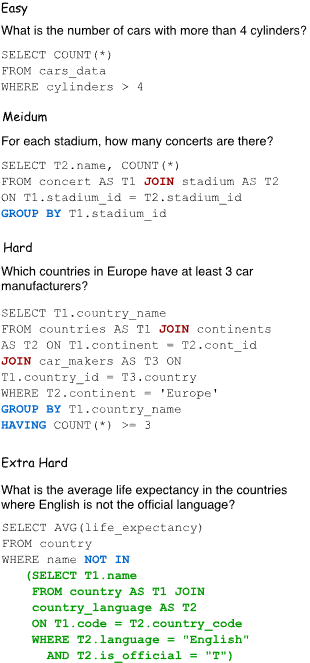
\includegraphics[width=0.35\textwidth]{image.png}
\caption{SQL query examples in 4 hardness levels. Credit: Spider [1]}
\label{fig:hardness-levels}
\end{figure}

\subsection{Prompting and Input}
\label{sec:prompting}

Each model receives three pieces of information in a single zero-shot user turn: a system instruction explaining its role as a Text-to-SQL generator, the database schema (table names, column names, primary keys, and foreign-key relationships, with no example rows), and the natural-language question. No few-shot examples are provided, so that the experiment measures each model's ability to generate SQL from instructions and schema information alone, without the confound of examples steering its output style. The prompt template is identical across all three models, so that differences in performance can be attributed to the models rather than to differences in prompting.

\textbf{Prompt template:}
\begin{verbatim}
Given the following SQLite database schema, write a SQL query that answers
the question.

{schema}

Question: {question}

Respond with only the SQL query in a ```sql code block.
\end{verbatim}

See \hyperref[sec:appendix1]{Appendix 1} for a worked example: a full schema, a question, and the resulting filled prompt.

\subsection{SQL Extraction}
\label{sec:sql-extraction}

For each sample, we decode the model's generated tokens into text using the model-specific tokenizer, and check for the presence of a \texttt{</think>} token. If \texttt{</think>} was generated, we take all text generated before \texttt{</think>} as the reasoning trace and all text to the right as the output SQL; DeepSeek-R1-Distill-Qwen-1.5B is the only model of the three that can emit this token. The SQL is then extracted from the first \texttt{```sql} code block in that remaining text. The extracted SQL is passed to the evaluation script as-is. Outputs that cannot be extracted or parsed are counted as incorrect on every metric rather than excluded from the evaluation, as unusable output is a task failure (see \ref{sec:evaluation-metrics} and \ref{sec:invalid-outputs}).

\subsection{Inference Settings}
\label{sec:inference-settings}

All models are evaluated using the same decoding configuration: greedy decoding (temperature and top-p are not applicable) for consistent, reproducible results between runs. The maximum output length differs by model: 256 tokens for Qwen3-0.6B, and 4096 tokens for both Qwen3-4B and DeepSeek-R1-Distill-Qwen-1.5B. For DeepSeek, the larger budget is needed because its output also has to contain a full reasoning trace rather than only the SQL query; Qwen3-4B is given the same, larger budget as DeepSeek so that a tighter token limit can be ruled out as the reason for any difference between them on invalid-output rate (\ref{sec:invalid-outputs}) or inference time (\ref{sec:efficiency}). Qwen3-0.6B and Qwen3-4B are both run with thinking mode off (both support it). DeepSeek-R1-Distill-Qwen-1.5B always produces a reasoning trace and has no documented way to disable thinking mode, so it is evaluated as the reasoning condition against the two non-reasoning Qwen3 models. All inference runs on the same 1x RTX 4090 GPU described in \ref{sec:models}, with batch size 1.

\subsection{Evaluation}
\label{sec:evaluation-metrics}

We evaluate the output using the same metrics as the Spider paper [1]. These are:

\begin{enumerate}
\item Component Matching
    \begin{itemize}
        \item For each of the following components:
        \begin{itemize}
            \item SELECT
            \item WHERE
            \item GROUP BY
            \item ORDER BY
            \item KEYWORDS (including all SQL keywords without column names and operators)
        \end{itemize}
        \item Decompose each component in the prediction and ground truth as bags of several sub-components and check whether or not these two sets of components match completely.
        \item Checks accuracy, recall, and F1
    \end{itemize}
\item Exact Matching Accuracy
    \begin{itemize}
        \item We measure whether the generated query as a whole is equivalent to the last section
        \item The generated query is correct only if all components are correct
        \item Checks only accuracy
    \end{itemize}
\item Execution Accuracy
    \begin{itemize}
        \item A list of gold values for each question is given
        \item We measure how many gold values the generated query extracts when executed
        \item Checks only accuracy
    \end{itemize}
\end{enumerate}

If output is invalid or unparsable, then it fails all 3 dimensions (component matching, exact matching, execution accuracy), consistent with how \ref{sec:sql-extraction} extracts and passes SQL to this evaluation script. This is reasonable as invalid/unparsable output cannot be applied to SQL and thus must be avoided and penalized heavily; Results~\ref{sec:invalid-outputs} reports how often this happens for each model.

\section{Task 1 -- RQ1: Results}
\label{sec:rq1-results}

\subsection{Overall Model Performance}
\label{sec:overall-performance}

Below we report how Qwen3-0.6B, Qwen3-4B, and Deepseek-R1-Distill-Qwen3-1.5B perform on the Spider benchmark across all 3 metrics (Component Matching, Exact Matching Accuracy, Execution Accuracy). We calculate the values per problem difficulty as well as overall, and display them in the below tables.

\begin{table}[H]
\centering
\footnotesize
\caption{Overall performance summary, aggregated across all difficulties (all 1034 problems). Component matching is accuracy / recall / F1 (macro-averaged, see the note on table~\ref{tab:difficulty-component} in \ref{sec:rq1-interpretation}). Per-difficulty breakdowns are in tables~\ref{tab:difficulty-component}--\ref{tab:difficulty-execution}.}
\label{tab:overall-performance}
\resizebox{\textwidth}{!}{%
\begin{tabular}{lllccc}
\toprule
Model & Parameters & Category & Component matching & Exact matching & Execution accuracy \\
\midrule
Qwen3-0.6B & 0.6B & Decoder-only & 0.628 / 0.209 / 0.314 & 0.099 & 0.209 \\
Qwen3-4B & 4B & Decoder-only & 0.797 / 0.306 / 0.442 & 0.256 & 0.353 \\
DeepSeek-R1-Distill-Qwen-1.5B & 1.5B & Reasoning & 0.661 / 0.174 / 0.275 & 0.085 & 0.121 \\
\bottomrule
\end{tabular}}
\end{table}

All models are evaluated zero-shot with the same prompt on the 20 databases of the Spider dev set. Aggregated across all difficulties and databases, every model is still far from solving the task: execution accuracy ranges from 0.121 (DeepSeek) to 0.353 (Qwen3-4B) and exact matching accuracy from 0.085 (DeepSeek) to 0.256 (Qwen3-4B). Execution accuracy is higher than exact matching accuracy for all three models (for example 0.353 vs.\ 0.256 for Qwen3-4B), which suggests that at least some of the queries that return the correct result are written differently from the gold SQL (see \ref{sec:rq1-interpretation} for more on this relationship). Of the three models, Qwen3-4B is now the best on almost every metric, database, and difficulty level; \ref{sec:by-database} and \ref{sec:rq1-interpretation} quantify how consistently. Table~\ref{tab:inference-time} reports the efficiency side of this comparison: inference time per example.

\subsection{Performance by Query Difficulty}
\label{sec:by-difficulty}

\begin{table}[H]
\centering
\footnotesize
\caption{Component matching (accuracy / recall / F1) by difficulty.}
\label{tab:difficulty-component}
\begin{tabular}{lcc}
\toprule
Model & easy & medium \\
\midrule
Problems (n) & 248 & 446 \\
Qwen3-0.6B & 0.675 / 0.308 / 0.423 & 0.582 / 0.235 / 0.334 \\
Qwen3-4B & 0.838 / 0.574 / 0.681 & 0.670 / 0.306 / 0.420 \\
DeepSeek-R1-Distill-Qwen-1.5B & 0.566 / 0.288 / 0.382 & 0.642 / 0.185 / 0.287 \\
\bottomrule
\end{tabular}

\vspace{0.5em}

\begin{tabular}{lccc}
\toprule
Model & hard & extra & all \\
\midrule
Problems (n) & 174 & 166 & 1034 \\
Qwen3-0.6B & 0.540 / 0.141 / 0.223 & 0.578 / 0.160 / 0.250 & 0.628 / 0.209 / 0.314 \\
Qwen3-4B & 0.796 / 0.262 / 0.394 & 0.485 / 0.150 / 0.229 & 0.797 / 0.306 / 0.442 \\
DeepSeek-R1-Distill-Qwen-1.5B & 0.543 / 0.113 / 0.187 & 0.389 / 0.104 / 0.164 & 0.661 / 0.174 / 0.275 \\
\bottomrule
\end{tabular}
\end{table}

\begin{table}[H]
\centering
\footnotesize
\caption{Exact matching accuracy by difficulty.}
\label{tab:difficulty-exact}
\begin{tabular}{lccccc}
\toprule
Model & easy & medium & hard & extra & all \\
\midrule
Problems (n) & 248 & 446 & 174 & 166 & 1034 \\
Qwen3-0.6B & 0.157 & 0.137 & 0.006 & 0.006 & 0.099 \\
Qwen3-4B & 0.508 & 0.262 & 0.115 & 0.012 & 0.256 \\
DeepSeek-R1-Distill-Qwen-1.5B & 0.214 & 0.078 & 0.000 & 0.000 & 0.085 \\
\bottomrule
\end{tabular}
\end{table}

\begin{table}[H]
\centering
\footnotesize
\caption{Execution accuracy by difficulty.}
\label{tab:difficulty-execution}
\begin{tabular}{lccccc}
\toprule
Model & easy & medium & hard & extra & all \\
\midrule
Problems (n) & 248 & 446 & 174 & 166 & 1034 \\
Qwen3-0.6B & 0.210 & 0.276 & 0.126 & 0.114 & 0.209 \\
Qwen3-4B & 0.565 & 0.345 & 0.276 & 0.139 & 0.353 \\
DeepSeek-R1-Distill-Qwen-1.5B & 0.258 & 0.128 & 0.017 & 0.006 & 0.121 \\
\bottomrule
\end{tabular}
\end{table}

We break every metric down by the Spider Hardness Criteria (\ref{sec:eval-data}) as query difficulty is a first-order driver of Text-to-SQL performance; comparing models only in aggregate would hide whether a model's advantage holds up as queries get harder.

Performance decreases with difficulty for every model, but the decrease is steepest for Qwen3-0.6B and DeepSeek: their exact matching and execution accuracy are both at most 0.034 and 0.126 respectively on hard and extra problems, down from as high as 0.210-0.258 (easy execution) on the easiest problems (table~\ref{tab:difficulty-exact} and table~\ref{tab:difficulty-execution}). Qwen3-4B degrades on the same relative scale but from a much higher starting point, from 0.508 easy exact matching / 0.565 easy execution accuracy down to 0.012 extra exact matching / 0.139 extra execution accuracy. Despite the degredation, it remains the best of the three models at every single difficulty level on both metrics (tables~\ref{tab:difficulty-exact}--\ref{tab:difficulty-execution}).

\subsection{Performance by Database}
\label{sec:by-database}

We also break execution and exact matching accuracy down by each of the 20 Spider dev databases. Qwen3-4B has the highest execution accuracy on 17 of the 20 databases outright (plus a tie on one more) and the highest exact matching accuracy on 18 of 20, while DeepSeek-R1-Distill-Qwen-1.5B is never highest on either metric; Qwen3-0.6B wins outright only on orchestra and battle\_death. Databases with few problems (real\_estate\_properties with n=4, voter\_1 with n=15, battle\_death with n=16, and museum\_visit with n=18) are too small to rank the models reliably, since a single problem changes a score by 6 to 25 percentage points. Execution accuracy ranges from 0.10 (course\_teach) to 0.53 (singer) for Qwen3-0.6B, from 0.19 (battle\_death) to 0.60 (singer) for Qwen3-4B, and from 0.00 (concert\_singer) to 0.27 (singer and voter\_1) for DeepSeek-R1-Distill-Qwen-1.5B (\hyperref[tab:db-execution]{Table 5}). The pattern on exact matching accuracy is just as one-sided (\hyperref[tab:db-exact]{Table 6}): Qwen3-4B is highest on 18 of 20 databases, ties Qwen3-0.6B on orchestra, and loses only on battle\_death; DeepSeek's exact matching accuracy is never the highest of the three, coming closest on flight\_2 (0.200 vs.\ Qwen3-4B's 0.350 and Qwen3-0.6B's 0.075). The full per-database tables and discussion are in \hyperref[sec:appendix2]{Appendix 2}.

\subsection{Invalid and Unparseable Outputs}
\label{sec:invalid-outputs}

We also count how often each model's output cannot be used as SQL at all: it either never produces a usable query within the token budget (\ref{sec:inference-settings}) or is truncated before finishing one. Per \ref{sec:evaluation-metrics}, these count as failures on every metric rather than being excluded, and this is a direct measure of how reliably each model follows the ``respond with only a SQL query'' instruction, independent of whether the SQL it does produce is correct. Qwen3-0.6B's invalid rate is 2.2\%, Qwen3-4B's is 0.0\%, and DeepSeek-R1-Distill-Qwen-1.5B's is 9.7\%, about 4x higher than Qwen3-0.6B's despite having the same 4096-token budget as Qwen3-4B (\ref{sec:inference-settings}), i.e. a larger token budget did not cause Qwen3-4B to run on or produce unusable output the way it does for DeepSeek. \ref{sec:rq1-interpretation} breaks DeepSeek's failures down further by difficulty and by why the generation failed (tables~\ref{tab:deepseek-outcome}--\ref{tab:deepseek-unfinished-by-difficulty}).

\subsection{Efficiency Measures}
\label{sec:efficiency}

\begin{table}[H]
\centering
\footnotesize
\caption{Output tokens per example}
\label{tab:tokens-per-example}
\begin{tabular}{lccccc}
\toprule
Model & easy & medium & hard & extra & all \\
\midrule
Qwen3-0.6B & 27.5 & 44.7 & 53.7 & 69.9 & 46.1 \\
Qwen3-4B & 23.6 & 37.3 & 46.2 & 59.0 & 39.0 \\
DeepSeek-R1-Distill-Qwen-1.5B & 610.8 & 768.4 & 1096.0 & 1176.9 & 851.3 \\
\bottomrule
\end{tabular}
\end{table}

Inference time is measured from the start of generation to the complete batch output, per batch of 1 example, excluding tokenization, model loading, and warm-up.

\begin{table}[H]
\centering
\footnotesize
\caption{Inference time.}
\label{tab:inference-time}
\begin{tabular}{lcc}
\toprule
Model & Total wall time (s) & Avg.\ time per example (s) \\
\midrule
Qwen3-0.6B & 123.9 & 0.120 \\
Qwen3-4B & 109.1 & 0.106 \\
DeepSeek-R1-Distill-Qwen-1.5B & 3059.8 & 2.959 \\
\bottomrule
\end{tabular}
\end{table}

DeepSeek is about 25x slower per example than Qwen3-0.6B and 28x slower than Qwen3-4B, consistent with its much higher average token count (table~\ref{tab:tokens-per-example}). Qwen3-4B, despite having about 7x as many parameters as Qwen3-0.6B, is marginally faster per example (0.106s vs.\ 0.120s), consistent with it generating fewer tokens on average (39.0 vs.\ 46.1, table~\ref{tab:tokens-per-example}) despite having the same 16x larger token budget as DeepSeek (\ref{sec:inference-settings}).

\begin{table}[H]
\centering
\footnotesize
\caption{DeepSeek-R1-Distill-Qwen-1.5B by generation outcome. ``Cut'' means the generation reached the 4096-token limit.}
\label{tab:deepseek-outcome}
\begin{tabular}{lccccc}
\toprule
Outcome & Problems (n) & Share & Avg.\ tokens & Exact match & Component F1 \\
\midrule
Finished with SQL & 934 & 90.3\% & 512 & 0.094 & 0.286 \\
Finished, no usable SQL & 2 & 0.2\% & 284 & 0.000 & 0.100 \\
Cut while answering (after \texttt{</think>}) & 13 & 1.3\% & 4096 & 0.000 & 0.096 \\
Cut while thinking (no \texttt{</think>}) & 85 & 8.2\% & 4096 & 0.000 & 0.093 \\
All & 1034 & 100\% & 851 & 0.085 & 0.275 \\
\bottomrule
\end{tabular}
\end{table}

\begin{table}[H]
\centering
\footnotesize
\caption{The same 934 questions that DeepSeek finished, for all three models.}
\label{tab:deepseek-finished-934}
\begin{tabular}{lcc}
\toprule
Model & Exact match & Component F1 \\
\midrule
DeepSeek-R1-Distill-Qwen-1.5B & 0.094 & 0.286 \\
Qwen3-0.6B & 0.103 & 0.317 \\
Qwen3-4B & 0.257 & 0.440 \\
\bottomrule
\end{tabular}
\end{table}

\begin{table}[H]
\centering
\footnotesize
\caption{Are the cut-off DeepSeek generations infinite self-repetition loops? A text that repeats itself compresses well, so a low compression ratio of the last 3000 characters indicates a loop.}
\label{tab:deepseek-repetition}
\begin{tabular}{lcccc}
\toprule
Generations & n & Median compression ratio & Ratio $<$ 0.15 & Last 150 characters repeat 3 or more times \\
\midrule
Cut off & 98 & 0.095 & 95.9\% & 96.9\% \\
Finished & 936 & 0.418 & 0.0\% & 0.2\% \\
\bottomrule
\end{tabular}
\end{table}

\begin{table}[H]
\centering
\footnotesize
\caption{Share of DeepSeek generations that did not finish with SQL, by difficulty.}
\label{tab:deepseek-unfinished-by-difficulty}
\begin{tabular}{lccccc}
\toprule
 & easy & medium & hard & extra & all \\
\midrule
Problems (n) & 248 & 446 & 174 & 166 & 1034 \\
Not finished with SQL (n) & 15 & 33 & 25 & 27 & 100 \\
Share & 6.0\% & 7.4\% & 14.4\% & 16.3\% & 9.7\% \\
\bottomrule
\end{tabular}
\end{table}

\section{Interpretation and Answer to Research Question (RQ1)}
\label{sec:rq1-interpretation}

\textbf{RQ1:} How do (selected) LLMs perform on cross-domain Text-to-SQL?

\vspace{10px}

All three models are still far from solving the task in this zero-shot setting: exact matching accuracy ranges from 0.085 to 0.256 and execution accuracy from 0.121 to 0.353 (table~\ref{tab:overall-performance}). Difficulty and database effects are discussed in \ref{sec:by-difficulty} and \ref{sec:by-database}; here we interpret the effects of model size and reasoning architecture and the exact-match/execution-accuracy relationship, and state the answer to RQ1 as three findings.

\textbf{First, within the Qwen family, scale is a strong and almost uniform predictor of performance, but an intermediate-size reasoning model from the Deepseek family still loses to the smallest model in the Qwen family.} Aggregated across all difficulties, Qwen3-4B has the best component matching (0.797 / 0.306 / 0.442), exact matching (0.256), and execution accuracy (0.353) of the three (table~\ref{tab:overall-performance}), and it beats Qwen3-0.6B on exact matching and execution accuracy at every individual difficulty level, including hard (0.115 vs.\ 0.006) and extra (0.012 vs.\ 0.006), where the smaller model solves almost nothing (tables~\ref{tab:difficulty-exact}--\ref{tab:difficulty-execution}). This is the largest, most consistent effect in the RQ1 results. The one exception is component matching on extra-hard problems, where Qwen3-0.6B's accuracy, recall, and F1 (0.578 / 0.160 / 0.250) are all slightly higher than Qwen3-4B's (0.485 / 0.150 / 0.229), the only point in the RQ1 results where the smaller Qwen3 model wins outright (table~\ref{tab:difficulty-component}). DeepSeek-R1-Distill-Qwen-1.5B sits between the two Qwen3 models in parameter count (1.5B) and is the only one that reasons, yet it is the lowest of the three on every aggregate metric (0.275 component F1, 0.085 exact matching, 0.121 execution accuracy) except its own component-matching accuracy (0.661 vs.\ 0.628 for Qwen3-0.6B). Thus, scale predicts performance well within a family, but does not transfer across the reasoning/non-reasoning boundary: having more parameters than Qwen3-0.6B did not help DeepSeek catch up to it.

\textbf{Second, the reasoning architecture itself, not parameter count, is the main driver of DeepSeek's low score.} Its invalid-output rate (9.7\%) is markedly higher than Qwen3-0.6B's (2.2\%) and Qwen3-4B's (0.0\% in this run) (\ref{sec:invalid-outputs}). In tables~\ref{tab:deepseek-outcome}--\ref{tab:deepseek-unfinished-by-difficulty}, 100 of 1034 generations (9.7\%) end without usable SQL. 85 never leave the reasoning phase, 13 are cut while writing the answer, and 2 finish without SQL. The number of unusable SQL generations also grows with difficulty, from 6.0\% on easy to 16.3\% on extra problems. These are not cases of long productive reasoning either: 95.9\% of the cut-off generations are highly self-repetitive (compression ratio below 0.15, median compression ratio 0.095, vs.\ 0.418 for finished generations), rewriting the same query and repeating phrases like ``So the final query is:'' without converging. Finishing does not make it better either: on the 934 questions DeepSeek does finish, its exact matching (0.094) and component F1 (0.286) are still below Qwen3-0.6B's on the same questions (0.103 / 0.317) and far below Qwen3-4B's (0.257 / 0.440), despite generating 512 tokens per question on average there, against 46 and 39 tokens overall for Qwen3-0.6B and Qwen3-4B (about 18x and 22x fewer). This extra length also costs time: DeepSeek is 25-28x slower per example than either Qwen3 model (\ref{sec:efficiency}). The reasoning trace mostly lengthens the output and sometimes never terminates, without improving the SQL when it does, and size alone is not the explanation, since Qwen3-4B is both bigger than DeepSeek and the best model in the comparison. Thus, reasoning architecture itself, not the parameter count, is the main driver of DeepSeek's low score.

\textbf{Third, query difficulty has a substantial, consistent effect on every model, including the best one.} Exact matching and execution accuracy both fall sharply from easy to extra-hard problems for all three models (\ref{sec:by-difficulty}). Qwen3-4B's drop is from a much higher base (0.508 to 0.012 exact matching, 0.565 to 0.139 execution accuracy) and it remains the best model at every difficulty level on both metrics, but the drop itself is just as steep in relative terms as for the other two models, and the hardest problems remain largely unsolved even for it.

\textbf{Exact match vs.\ execution accuracy.} For all three models, execution accuracy aggregated across all difficulties exceeds exact matching accuracy (table~\ref{tab:overall-performance}): 0.209 vs.\ 0.099 for Qwen3-0.6B, 0.353 vs.\ 0.256 for Qwen3-4B, and 0.121 vs.\ 0.085 for DeepSeek. Since exact matching requires every SQL component to match the gold query while execution accuracy only requires the same result set, this gap indicates each model writes some queries that are valid and correct but phrased differently from the gold SQL (e.g.\ a different but equivalent join order, or an explicit column list where the gold query uses \texttt{SELECT *}). The gap is widest for Qwen3-0.6B (11.0 points), close behind for Qwen3-4B (9.7 points), and narrowest for DeepSeek (3.6 points); DeepSeek's narrower gap reflects it producing fewer alternative-but-valid queries. Qwen3-4B's gap is almost as wide as Qwen3-0.6B's despite much higher absolute accuracy, so scaling up within the Qwen3 family raises both Exact Match Accuracy and Execution Accuracy together rather than closing the gap between them.

\textbf{Limitations.} Our working hypothesis is that Text-to-SQL at this scale does not benefit from an explicit reasoning trace, and that a non-reasoning model is sufficient, with performance instead scaling with parameter count within a fixed model family. The results are consistent with this hypothesis. However, they do not establish that Text-to-SQL is too simple for reasoning models in general due to several factors:

\begin{itemize}
\item \textbf{Truncation and failed outputs for DeepSeek.} These count as failures on every metric and lower its recall, exact matching, and execution scores, but table~\ref{tab:deepseek-finished-934} shows removing them would not change the ranking (DeepSeek is also lower on the questions it finished), and table~\ref{tab:deepseek-repetition} shows the cut-off generations are repetition loops, so a larger token budget is unlikely to rescue them.
\item \textbf{Model differences beyond reasoning.} Qwen3-0.6B and Qwen3-4B share a model family, isolating the effect of scale between them, but DeepSeek differs from both in family, size, and pretraining/post-training, not only in whether it reasons; it is also a distilled model, so the effect of reasoning cannot be fully separated from distillation quality.
\item \textbf{Aggregated component matching.} The component matching figures in table~\ref{tab:difficulty-component} (and in table~\ref{tab:overall-performance}) are our own macro-average (mean of the 10 per-component accuracy and recall scores, with F1 computed from these two means), not a number reported by Spider.
\end{itemize}

Overall, in this zero-shot, cross-domain setting, a larger non-reasoning decoder-only model (Qwen3-4B, 4B) clearly outperforms both a same-family model at under a sixth its size (Qwen3-0.6B) and a reasoning model of intermediate size from a different family (DeepSeek-R1-Distill-Qwen-1.5B, 1.5B), while also being faster per example than either. None of the three models solve more than half of even the easiest problems or more than a small fraction of hard or extra-hard queries. This answers RQ1 for the three models evaluated.
 (this
% file links back into Task 1's tab:overall-performance and sec:rq1-results
% labels).
%
% Annotations made while converting this to reference-based numbering:
%  - \section*{Task 3 -- RQ3: Methodology}, \section*{Task 3 -- RQ3:
%    Results}, and \subsection*{Task 3 -- RQ3: Extension to Qwen3-4B} became
%    real, numbered \section/\subsection commands with \label. The
%    Extension subsection's title had "Task 3 -- RQ3: " stripped, since
%    that's now implied by nesting under the numbered Task 3 section
%    (matching how RQ1.tex strips the old manual "1.1"/"2.2" prefixes).
%  - Tables 16, 17, 18, 21, 22, 23, 24 each got a \label; every in-text
%    "Table 16/17/18/21/22/24" mention, including the forward reference
%    from Table 16's own caption to Table 18, became a \ref.
%  - Mentions of "Task 1" results now link to RQ1.tex's own labels
%    (sec:rq1-results, tab:overall-performance) via \hyperref, so they stay
%    live links even though Task 1's own numbering changed when RQ1.tex was
%    built.
%  - PRE-EXISTING ISSUE, NOT INTRODUCED HERE: Table 23's caption says
%    "Settings as in Table 19", and the "Longer training and
%    hyperparameters" paragraph discusses a 0.6B long-training sweep
%    (h0/h4/h5/h6, "the best long 0.6B run (0.613 / 0.632)") that has no
%    corresponding table anywhere in this document -- there is no Table 19
%    or Table 20 to point to. This looks like a 0.6B sweep table (the
%    equivalent of Table 23 for 0.6B) was planned/removed but the reference
%    to it was never updated. Left as plain, unlinked text "Table 19" since
%    there's nothing real to \ref; flagging for the author to either add
%    the missing table or fix the caption.

\section{Task 3 -- RQ3: Methodology}
\label{sec:rq3-methodology}

\textbf{RQ3:} To what extent does PlanPlay-SQL improve Qwen3-0.6B?

We improve Qwen3-0.6B [2] with thinking disabled, the same configuration as in \hyperref[sec:rq1-results]{Task 1}. We chose it because our compute is limited to a single RTX 4090, and iterative training on DeepSeek-R1-Distill-Qwen-1.5B would mean sampling and training on traces of about 850 tokens per question. Qwen3-0.6B generates about 46 tokens per question, so we can sample and train over the whole Spider training split. It also looked promising in Task 1, with the highest execution accuracy (0.209) and the shortest outputs. Task 1's execution accuracy is measured on schema-only databases (no rows), so it is not directly comparable to the mock-database execution accuracy reported for Task 3 below; we re-evaluated the original model on the mock databases as well (table~\ref{tab:rq3-dev-results-06b}, ``Original (Task 1)'' row, 0.130) so that the Task 3 comparison between original and adapted models is apples-to-apples. We call our method \textbf{PlanPlay-SQL}: the model first writes a short \emph{plan}, then is trained by verified self-\emph{play}. It combines three ideas from recent work on small-model Text-to-SQL. From [7] and [6], the model writes a short plan (tables and joins, columns, filters, aggregation and ordering) before the SQL, which gives a model with no thinking mode a place to organize the schema. We then fine-tune on the Spider training split in three stages, following [5]. First, a supervised warm start on gold SQL. Second, verification-based iterative fine-tuning: the model answers training questions, we execute its SQL and the gold SQL, keep the answers with matching results as positives, and fine-tune on them. Third, self-play fine-tuning: using the logistic loss of SPIN [8], we train the best checkpoint to prefer a verified correct answer over an incorrect answer produced by the worst checkpoint. Training uses only the Spider training split, and checkpoints are selected on held-out training databases, so the dev set stays untouched and evaluation stays cross-domain. We skip [5]'s synthetic question generation because Spider already provides gold SQL to execute against.

We expect PlanPlay-SQL to improve performance in two ways. The warm start teaches the model Spider's schema conventions and output style, which should raise exact and execution accuracy most, since Task 1 showed that many of the model's outputs are valid SQL that differs from the gold query. The verification and self-play stages then train on the model's own execution-checked outputs, which should reduce its remaining execution errors. We expect most of the gain to come from the warm start. Paper [5] found that verification-based fine-tuning gave most of its gains and self-play only a further 0.6 to 0.8 points, on much larger models, so self-play may add little at 0.6B. To measure each part, we report five rows on the same dev set and metrics as \hyperref[sec:rq1-results]{Task 1}: the original solution, the plan prompt only, the warm start only, warm start plus verification fine-tuning, and the full PlanPlay-SQL.

Gold SQL has no plan annotation, so the warm-start target is generated, not written by hand: a rule-based parser reads each gold query's top-level clauses (FROM/JOIN, SELECT, WHERE, GROUP BY/ORDER BY/LIMIT, and any set operator) with a small regex-based SQL splitter and renders them into the five-line plan format shown in the prompt template below. The parser is deterministic and derived purely from the gold SQL text; no model or human writes these training-target plans.

All stages use LoRA adapters (rank 32, alpha 64) on top of the frozen base checkpoint, rather than full fine-tuning. Table~\ref{tab:rq3-training-settings} below gives the learning rate, epochs, batch size, and training-item counts actually used for each stage; all stages share seed 0 and the same 707-question, 20-database held-out validation set described in \ref{sec:rq3-results}. ``Samples per question'' (k) is the number of candidate SQL completions sampled per training question during verification-based and self-play fine-tuning, before the correctness filter is applied; the resulting training-item count after filtering is reported in the ``training items'' column, since not every sampled question yields a usable positive or preference pair.

\begin{table}[H]
\centering
\footnotesize
\caption{Training settings for each stage in table~\ref{tab:rq3-validation-accuracy-06b}. Learning rate is the peak LR under a linear schedule.}
\label{tab:rq3-training-settings}
\resizebox{\textwidth}{!}{%
\begin{tabular}{lllccccc}
\toprule
Stage (table~\ref{tab:rq3-validation-accuracy-06b} row) & Init checkpoint & Training items & Samples/question (k) & Learning rate & Epochs & Batch size & Rounds \\
\midrule
Warm start (plan format, 1500 gold) & Qwen3-0.6B & 1500 gold SQL+plan pairs & --- & 2e-4 & 3 & 32 & 1 \\
+ 1500 further gold (supervised control) & Warm start & 1500 gold SQL+plan pairs & --- & 1e-4 & 1 & 32 & 1 \\
+ VBI-FT (same 1500 questions, hard only) & Warm start & 476 verified positives (of 1500 sampled) & 4 & 1e-4 & 1 & 32 & 1 \\
+ self-play, lower LR & VBI-FT (800-question round) & 279 verified preference pairs (of 800 sampled) & 4 & 1e-5 & 1 & 32 & 1 of 2 planned \\
+ self-play, higher LR & Warm start & 727 verified preference pairs (of 1500 sampled) & 4 & 1e-4 & 2 & 32 & 1 \\
\bottomrule
\end{tabular}}
\end{table}

\section{Task 3 -- RQ3: Results}
\label{sec:rq3-results}

Table~\ref{tab:rq3-dev-results-06b} compares the original Qwen3-0.6B from \hyperref[sec:rq1-results]{Task 1} with the adapted model on the same 1034 Spider dev questions, with the same metrics and the same execution-checking databases. The adapted model uses the plan-then-SQL prompt, greedy decoding, and a maximum of 384 new tokens (Task 1: 256). Execution accuracy is computed on mock databases (see the limitations below), so we treat exact matching accuracy as the more reliable number.

\begin{table}[H]
\centering
\footnotesize
\caption{Original and adapted Qwen3-0.6B on the Spider dev set, overall and by difficulty. Component matching is accuracy / recall / F1 (macro-averaged as in \hyperref[sec:rq1-interpretation]{Task 1}). Execution accuracy is on mock databases.}
\label{tab:rq3-dev-results-06b}
\resizebox{\textwidth}{!}{%
\begin{tabular}{llccccc}
\toprule
Metric & Model & easy & medium & hard & extra & all \\
\midrule
Problems (n) & & 248 & 446 & 174 & 166 & 1034 \\
Component matching & Original (Task 1) & 0.675 / 0.308 / 0.423 & 0.582 / 0.235 / 0.334 & 0.540 / 0.141 / 0.223 & 0.578 / 0.160 / 0.250 & 0.628 / 0.209 / 0.314 \\
 & Adapted & 0.809 / 0.763 / 0.786 & 0.750 / 0.643 / 0.693 & 0.815 / 0.626 / 0.708 & 0.696 / 0.478 / 0.567 & 0.783 / 0.636 / 0.702 \\
Exact matching & Original (Task 1) & 0.157 & 0.137 & 0.006 & 0.006 & 0.099 \\
 & Adapted & 0.762 & 0.594 & 0.385 & 0.265 & 0.546 \\
Execution (mock DB) & Original (Task 1) & 0.173 & 0.179 & 0.029 & 0.036 & 0.130 \\
 & Adapted & 0.794 & 0.583 & 0.443 & 0.277 & 0.561 \\
\bottomrule
\end{tabular}}
\end{table}

The adapted model is better on every metric and every difficulty level. Exact matching accuracy rises from 0.099 to 0.546 overall, and the largest relative gains are on hard (0.006 to 0.385) and extra (0.006 to 0.265) problems, which the original model almost never solved. Component matching recall rises from 0.209 to 0.636, so the model now writes most of the components the gold query contains. Execution accuracy on the mock databases rises from 0.130 to 0.561. The model is still weak on queries with set operations and nesting: the INTERSECT/UNION/EXCEPT and nested-query component (IUEN) has an accuracy of only 0.288. Our expectation that adapting on the Spider training split would help held, with much larger gains than we expected from a 0.6B model.

To see which part of the method helps, table~\ref{tab:rq3-validation-accuracy-06b} reports accuracy on a held-out validation set of 707 questions from 20 training databases that were never used for training. This validation set was used for choosing checkpoints, and the dev set was not.

\begin{table}[H]
\centering
\footnotesize
\caption{Validation accuracy (execution match on mock databases, 707 questions) after each stage. The row marked * uses a 300-question subset of the same validation set.}
\label{tab:rq3-validation-accuracy-06b}
\begin{tabular}{lc}
\toprule
Stage & Validation accuracy \\
\midrule
Base model, original prompt* & 0.407 \\
Base model, plan prompt, no training* & 0.050 \\
Warm start on 1500 gold questions (plan format) & 0.622 \\
+ 1500 further gold questions (supervised control) & 0.652 \\
+ VBI-FT on the same 1500 questions (no gold SQL, hard questions only, 476 verified samples) & 0.651 \\
+ self-play, lower learning rate (1e-5, 9 steps) & 0.631 \\
+ self-play, higher learning rate (1e-4, 46 steps) & 0.034 \\
\bottomrule
\end{tabular}
\end{table}

The warm start accounts for most of the gain (0.407 to 0.622). The plan prompt without training does very poorly (0.050), so the plan format only helps after fine-tuning. Verification-based fine-tuning matched the supervised control (0.651 vs.\ 0.652, a difference far smaller than the roughly 2-point sampling error of 707 questions) while using only 476 self-generated, execution-verified training items instead of 1500 gold ones and no gold SQL text. Self-play did not help: with a low learning rate it barely changed the model (0.622 to 0.631), and with a higher learning rate the training loss fell from 0.69 to 0.25 but accuracy collapsed to 0.034 with most outputs failing to execute. This matches the expectation from [5] that self-play adds little on top of verification-based fine-tuning, but it is more negative than the 0.6 to 0.8 points reported there. We report this as our final self-play result rather than rerunning with intermediate checkpointing and a lower learning rate: the lower-learning-rate run above already shows self-play adding at most 0.009 accuracy at this scale, so the higher-learning-rate collapse is a well-motivated negative finding about self-play's sensitivity on a 0.6B model, consistent with (and more pronounced than) [5]'s own small gains on larger models, rather than an open question that a rerun would likely overturn.

\textbf{Examples.} Out of 1034 dev questions, the adapted model gets 260 right that the original got wrong, loses 54 that the original got right, and both get 313 right (execution match on mock databases). One fixed example is the network\_1 question ``Show the student IDs and numbers of friends corresponding to each.'' The original model wrote \texttt{SELECT h.ID, h.name, h.grade, f.friend\_id FROM Highschooler h JOIN Friend f ON h.ID = f.student\_id}, which lists friends instead of counting them. The adapted model first wrote the plan \texttt{tables: friend; select: student\_id , count(*); group/order: group by student\_id} and then \texttt{SELECT student\_id , count(*) FROM friend GROUP BY student\_id}, which matches the gold query. One broken example is the tvshow question ``What are the titles of the cartoons sorted alphabetically?'' The original model wrote a correct query (\texttt{SELECT Title FROM Cartoon ORDER BY Title ASC}), but the adapted model's plan misspelled the table name (\texttt{tables: CARTON}), and the SQL that followed inherited the error (\texttt{SELECT Title FROM CARTON ORDER BY Title}), which fails to run. In this case the plan step propagated a mistake into the final query.

\textbf{Limitations.}

\begin{itemize}
\item \textbf{Mock databases.} The official Spider database files with rows were not available, so we generated databases with random rows seeded from the literals in each question's gold query. Execution accuracy on them only approximates the official execution accuracy. For example, Task 1's execution accuracy for the original model drops from 0.209 on schema-only databases to 0.130 on the mock databases (table~\ref{tab:overall-performance}), because on empty databases every query that returns nothing counts as correct. Exact matching accuracy does not depend on the databases.
\item \textbf{One run per configuration, one seed}, with no confidence intervals. The validation differences between the supervised control and VBI-FT are within sampling error.
\item \textbf{Different prompt and token budget.} The adapted model uses a different prompt and a larger token budget than the original, so the gain combines fine-tuning, the plan format, and the longer limit.
\item \textbf{Not the full method on dev.} The dev-set results are for the supervised stages only. VBI-FT and self-play were compared on the validation set.
\end{itemize}

\subsection{Extension to Qwen3-4B}
\label{sec:rq3-extension-4b}

To see whether PlanPlay-SQL still helps a larger model, we repeated the main RQ3 experiments on Qwen3-4B [2] with thinking disabled. Everything except the base checkpoint is unchanged: the same code (\texttt{--base Qwen/Qwen3-4B}), prompts, plan targets, LoRA target modules, training questions, seed, 707-question validation set, Spider dev set and mock databases, with one H100 per run. The ``Original'' row is our \hyperref[sec:rq1-results]{Task 1} greedy run of Qwen3-4B (thinking off), re-scored on the mock databases in the same way as the 0.6B baseline. We ran the table~\ref{tab:rq3-validation-accuracy-06b} stages with the table~\ref{tab:rq3-training-settings} settings and the four sweep settings that mattered for 0.6B (h0, h4, h5, h6). We did not re-run h1-h3, which were the weakest 0.6B settings. A 3-epoch warm start takes about 16 minutes on 4B, and a 30-epoch run on 3000 questions about 2 hours 10 minutes.

\begin{table}[H]
\centering
\footnotesize
\caption{Original and adapted Qwen3-4B on the Spider dev set (1034 questions). Adapted = plan-format warm start, 3 epochs (table~\ref{tab:rq3-training-settings} settings). Component matching is accuracy / recall / F1 as in table~\ref{tab:rq3-dev-results-06b}. Execution accuracy is on mock databases.}
\label{tab:rq3-dev-results-4b}
\resizebox{\textwidth}{!}{%
\begin{tabular}{llccccc}
\toprule
Metric & Model & easy & medium & hard & extra & all \\
\midrule
Problems (n) & & 248 & 446 & 174 & 166 & 1034 \\
Component matching & Original (Task 1) & 0.838 / 0.574 / 0.681 & 0.670 / 0.306 / 0.420 & 0.796 / 0.262 / 0.394 & 0.485 / 0.150 / 0.229 & 0.797 / 0.306 / 0.442 \\
 & Adapted & 0.834 / 0.826 / 0.830 & 0.806 / 0.783 / 0.794 & 0.796 / 0.780 / 0.788 & 0.783 / 0.716 / 0.748 & 0.828 / 0.800 / 0.814 \\
Exact matching & Original (Task 1) & 0.508 & 0.262 & 0.115 & 0.012 & 0.256 \\
 & Adapted & 0.786 & 0.760 & 0.517 & 0.458 & 0.677 \\
Execution (mock DB) & Original (Task 1) & 0.524 & 0.283 & 0.213 & 0.078 & 0.296 \\
 & Adapted & 0.867 & 0.753 & 0.603 & 0.482 & 0.712 \\
\bottomrule
\end{tabular}}
\end{table}

\begin{table}[H]
\centering
\footnotesize
\caption{Validation accuracy (execution match on mock databases, 707 questions) after each stage, Qwen3-4B next to the Qwen3-0.6B numbers from table~\ref{tab:rq3-validation-accuracy-06b}. Rows marked * use the same 300-question subset as table~\ref{tab:rq3-validation-accuracy-06b}.}
\label{tab:rq3-validation-accuracy-4b}
\begin{tabular}{lcc}
\toprule
Stage & Qwen3-4B & Qwen3-0.6B \\
\midrule
Base model, original prompt* & 0.703 & 0.407 \\
Base model, plan prompt, no training* & 0.577 & 0.050 \\
Warm start on 1500 gold questions (plan format, 3 epochs) & 0.754 & 0.622 \\
+ 1500 further gold questions (supervised control) & 0.792 & 0.652 \\
+ VBI-FT on the same 1500 questions (hard questions only; 4B: 275 verified samples) & 0.762 & 0.651 \\
+ VBI-FT (800 questions, 0.767), then self-play, lower learning rate (1e-5) & 0.765 & 0.631 \\
+ self-play, higher learning rate (1e-4, 2 epochs) & 0.115 & 0.034 \\
\bottomrule
\end{tabular}
\end{table}

\begin{landscape}
\begin{table}[H]
\centering
\footnotesize
\caption{Qwen3-4B validation accuracy (707 questions) during 30-epoch plan-format warm starts, evaluated every 5 epochs. Settings as in Table 19. The 3-epoch warm start reached 0.755, 0.775 and 0.754 after epochs 1, 2 and 3.}
\label{tab:rq3-sweep-4b}
\resizebox{\linewidth}{!}{%
\begin{tabular}{lcccccccccccc}
\toprule
Run & LR & Batch & LoRA r/alpha & Train Qs & ep 5 & ep 10 & ep 15 & ep 20 & ep 25 & ep 30 & Best (epoch) & 0.6B best \\
\midrule
h0 (table~\ref{tab:rq3-training-settings} config) & 0.0002 & 32 & 32/64 & 1500 & 0.743 & 0.741 & 0.721 & 0.730 & 0.731 & 0.733 & 0.743 (5) & 0.641 \\
h4 (larger LoRA) & 0.0002 & 32 & 64/128 & 1500 & 0.709 & 0.762 & 0.738 & 0.744 & 0.750 & 0.751 & 0.762 (10) & 0.658 \\
h5 (2x data) & 0.0001 & 32 & 32/64 & 3000 & 0.765 & 0.754 & 0.745 & 0.737 & 0.740 & 0.744 & 0.765 (5) & 0.677 \\
h6 (larger LoRA + 2x data) & 0.0001 & 32 & 64/128 & 3000 & 0.745 & 0.760 & 0.778 & 0.784 & 0.778 & 0.778 & 0.784 (20) & 0.693 \\
\bottomrule
\end{tabular}}
\end{table}
\end{landscape}

\begin{table}[H]
\centering
\footnotesize
\caption{Qwen3-4B on the Spider dev set (1034 questions), exact matching / execution accuracy (mock databases).}
\label{tab:rq3-dev-sweep-4b}
\resizebox{\textwidth}{!}{%
\begin{tabular}{lccccc}
\toprule
Model & easy & medium & hard & extra & all \\
\midrule
Original (Task 1) & 0.508 / 0.524 & 0.262 / 0.283 & 0.115 / 0.213 & 0.012 / 0.078 & 0.256 / 0.296 \\
Adapted, table~\ref{tab:rq3-dev-results-4b} (3 epochs) & 0.786 / 0.867 & 0.760 / 0.753 & 0.517 / 0.603 & 0.458 / 0.482 & 0.677 / 0.712 \\
h4 (larger LoRA), 10 epochs & 0.863 / 0.899 & 0.722 / 0.724 & 0.598 / 0.695 & 0.470 / 0.494 & 0.694 / 0.724 \\
h4 (larger LoRA), 20 epochs & 0.859 / 0.891 & 0.751 / 0.749 & 0.575 / 0.626 & 0.452 / 0.536 & 0.699 / 0.728 \\
h4 (larger LoRA), 30 epochs & 0.867 / 0.903 & 0.753 / 0.749 & 0.569 / 0.638 & 0.446 / 0.548 & 0.700 / 0.735 \\
h5 (2x data), 10 epochs & 0.790 / 0.851 & 0.744 / 0.762 & 0.540 / 0.626 & 0.428 / 0.494 & 0.670 / 0.718 \\
h5 (2x data), 20 epochs & 0.851 / 0.895 & 0.774 / 0.767 & 0.569 / 0.655 & 0.422 / 0.530 & 0.701 / 0.741 \\
h5 (2x data), 30 epochs & 0.851 / 0.887 & 0.778 / 0.774 & 0.575 / 0.655 & 0.446 / 0.554 & 0.708 / 0.746 \\
h6 (both), 10 epochs & 0.867 / 0.887 & 0.740 / 0.724 & 0.540 / 0.644 & 0.428 / 0.512 & 0.687 / 0.716 \\
h6 (both), 20 epochs & 0.839 / 0.883 & 0.751 / 0.726 & 0.603 / 0.678 & 0.476 / 0.542 & 0.703 / 0.726 \\
h6 (both), 30 epochs & 0.843 / 0.887 & 0.760 / 0.735 & 0.632 / 0.684 & 0.458 / 0.536 & 0.710 / 0.731 \\
\bottomrule
\end{tabular}}
\end{table}

\textbf{Results.} PlanPlay-SQL also improves Qwen3-4B substantially. The 3-epoch warm start raises dev exact matching from 0.256 to 0.677 and execution accuracy on the mock databases from 0.296 to 0.712, with gains at every difficulty level. The extra-hard exact matching rises from 0.012 to 0.458, and the set-operation/nesting component (IUEN), the weakest component for 0.6B (0.288), reaches 0.471. The adapted 4B model is better than every 0.6B checkpoint, including the best long 0.6B run (0.613 / 0.632). The absolute gain is similar to 0.6B (+42 against +45 exact-matching points), but 4B starts much higher. Without training, the plan prompt still costs accuracy at 4B (0.577 against 0.703 with the original prompt), but far less than at 0.6B (0.050), because the larger model can follow the plan format from the prompt alone.

\textbf{Stages.} The ordering of the stages is the same as for 0.6B, with two differences. First, continued supervised training on 1500 further gold questions gives the largest gain after the warm start (0.754 to 0.792). Second, VBI-FT helps less than the gold control at 4B (0.762 against 0.792), whereas the two were tied at 0.6B. The 4B warm start already answers about 76\% of sampled training questions correctly, so with hard-only filtering only 198 of the 1500 questions produce a verified positive, and VBI-FT trains on 275 items instead of 476. Self-play behaves as at 0.6B: with a low learning rate it does not change accuracy (0.767 to 0.765), and with a high learning rate it collapses (0.115), with longer outputs (120 against about 75 tokens) and a third of them failing to execute.

\textbf{Longer training and hyperparameters.} Longer training helps 4B less than 0.6B. Training loss falls below 1e-3 by epoch 15 and rounds to zero by epoch 20 in every run, and on validation only h6 (larger adapter and 2x data) ends above the 3-epoch warm start's best epoch (0.784 at epoch 20 against 0.775). h0 and h5 peak at epoch 5 and then lose 1 to 2 points, and h4 peaks at epoch 10. As for 0.6B, h6 is the best setting on validation and has the fewest queries that fail to execute (error fraction about 0.02, against about 0.06 to 0.07 for h0, h4 and h5). On dev, the three long settings again end close together: at 30 epochs they reach 0.700 to 0.710 exact matching and 0.731 to 0.746 execution accuracy, 2 to 3 points above the 3-epoch model on both metrics. These differences between settings are below the roughly 1.4-point sampling error of the dev set. The validation and dev sets again disagree: h5 declines on validation after epoch 5 but improves on dev through epoch 30.

\textbf{Answer for RQ3 at 4B.} PlanPlay-SQL raises Qwen3-4B's dev exact matching from 0.256 to 0.677 with the 3-epoch warm start, and to 0.700--0.710 with 30-epoch runs, and execution accuracy on mock databases from 0.296 to 0.712 and 0.731--0.746. The supervised warm start provides almost all of the gain. As the base model gets stronger, verification-based fine-tuning finds fewer hard questions to learn from, and longer training adds only 2 to 3 points. Self-play gives no gain at either scale. The same limitations as above apply (mock databases, one seed, prompt and token-budget differences, intermediate checkpoints of 30-epoch schedules, and dev results only for the supervised stages). The 4B ``Original'' run used a 4096-token limit against 384 for the adapted model, and h1-h3 were not repeated at 4B.
 into REPORT.tex, after % RQ1.tex -- Task 1 / RQ1 section, factored out of REPORT.tex.
%
% Intended use: % RQ1.tex -- Task 1 / RQ1 section, factored out of REPORT.tex.
%
% Intended use: \input{RQ1.tex} into REPORT.tex in place of the current inline
% "Task 1 -- RQ1: Methodology & Results" / "Task 1 -- RQ1: Results" content.
% REPORT.tex already loads every package this fragment needs (booktabs, array,
% graphicx, float, caption, hyperref), so no extra preamble is required.
%
% Annotations made while converting this to reference-based numbering:
%  - All \subsection*{N.M ...} / \section*{...} became real, numbered
%    \section/\subsection commands with the leading "N.M" stripped from the
%    title text (LaTeX now generates it), each with a \label. The former
%    \subsection*{3. Interpretation...} is promoted to a top-level \section,
%    since it was already numbered as a peer of Parts 1 and 2, not a child
%    of Part 2.
%  - Every table/figure got a \label right after its \caption, and every
%    in-text "table 1", "tables 2-4", "2.2", "Appendix 2", etc. became a
%    \ref (or \hyperref for Appendix 2/3, which live outside this file --
%    see note below). Because the Models table (1.1) is now counted and the
%    Appendix 2/3 tables are not part of this file's sequential numbering,
%    the printed table numbers shift versus the pasted draft (e.g. "table 1"
%    -> Table 2, "table 8" -> Table 6); every mention uses \ref, so this is
%    self-consistent and will stay correct if tables move again.
%  - Fixed a leftover inconsistency in 1.5: the draft's 1.1 and 2.5 both
%    state batch size 1 (confirmed correct), but 1.5 still said "batch size
%    128" (leftover from an earlier draft) -- corrected to 1.
%  - Both TODOs in the pasted draft are resolved inline: 2.2 now cites
%    Tables 4-5 directly instead of a placeholder, and 2.3 now cites the
%    concrete per-database numbers from Appendix 2 (pulled from REPORT.tex's
%    existing Appendix 2 prose) instead of a placeholder.
%  - The Overall Performance table's caption promises "the note on table 2
%    in 3" (i.e. a note about macro-averaged component matching, to appear
%    in the Interpretation section), but the pasted draft's Limitations list
%    dropped that bullet (it only kept "Truncation" and "Model differences").
%    Restored the "Aggregated component matching" bullet from the prior
%    REPORT.tex draft so the caption's forward reference resolves to real
%    content; this is a content restoration, not just a labeling change,
%    so flagging it here. The other previously-present bullet ("Single run
%    and sample size") was NOT restored, since nothing in the new draft
%    points to it -- worth confirming with the author whether that drop was
%    intentional.
%  - Appendix 1/2/3 and their tables (5, 6, 7) live in REPORT.tex, outside
%    this file. REPORT.tex's appendix tables keep their existing manual
%    "Table 5/6/7:" caption numbering (renumbering them would require
%    restructuring the whole document's table order, which is out of scope
%    here); \label{tab:db-execution}, \label{tab:db-exact} and
%    \label{tab:invalid-outputs} were added to those tables in REPORT.tex
%    (additive only, no visible change) so this file can link to them.
%    Since their printed numbers are not auto-generated, this file links to
%    them with \hyperref[label]{5}-style calls (a real clickable link, with
%    text matching the manual number already in their caption) rather than
%    \ref (which would print whatever their true document-order table
%    number is, not 5/6/7).

\section{Task 1 -- RQ1: Methodology \& Results}
\label{sec:rq1-methods}

\textbf{RQ1:} How do (selected) LLMs perform on cross-domain Text-to-SQL?

In this report we evaluate the performance of decoder-only language models as well as reasoning LLMs on cross-domain SQL.

\subsection{Models}
\label{sec:models}

We compare two decoder-only LLMs from the same model family at different scales (Qwen3-0.6B and Qwen3-4B) against one reasoning LLM, so that the comparison isolates the effect of scale within a fixed family from the effect of an explicit reasoning trace, as much as a 3-model study can. All three are accessed as local inference over their bf16 Huggingface checkpoints on 1x NVIDIA GeForce RTX 4090 GPU (no API-based models), so that inference parameters are fully under our control (see \ref{sec:inference-settings}). We evaluate using batch sizes of 1.

\begin{table}[H]
\centering
\footnotesize
\caption{Models compared in RQ1.}
\label{tab:models}
\resizebox{\textwidth}{!}{%
\begin{tabular}{llllll}
\toprule
Model & Category & Parameters & Quantization & Access & Thinking mode \\
\midrule
Qwen3-0.6B [2] & Decoder-only & 0.6B & bf16 (none beyond release precision) & Local, Huggingface checkpoint & Disabled \\
Qwen3-4B [2] & Decoder-only & 4B & bf16 (none beyond release precision) & Local, Huggingface checkpoint & Disabled \\
DeepSeek-R1-Distill-Qwen-1.5B [4] & Reasoning & 1.5B & bf16 (none beyond release precision) & Local, Huggingface checkpoint & Always on (no disable option) \\
\bottomrule
\end{tabular}}
\end{table}

All three are dense (non-MoE) models, so no distinction between total and active parameters applies.

\subsection{Evaluation Data}
\label{sec:eval-data}

We use all 1034 examples in the Spider [1] development split, with no subsampling and therefore no sampling seed to report; every example is included, so the per-database counts below and the per-database results tables (\hyperref[tab:db-execution]{5} and \hyperref[tab:db-exact]{6}) enumerate exactly which examples are used. To evaluate cross-domain performance, we additionally report results separately for each of the 20 databases in the Spider dev set: world\_1 (120 problems), car\_1 (92), cre\_Doc\_Template\_Mgt (84), dog\_kennels (82), flight\_2 (80), student\_transcripts\_tracking (78), wta\_1 (62), tvshow (62), network\_1 (56), concert\_singer (45), pets\_1 (42), poker\_player (40), orchestra (40), employee\_hire\_evaluation (38), course\_teach (30), singer (30), museum\_visit (18), battle\_death (16), voter\_1 (15), and real\_estate\_properties (4).

We also use the Spider Hardness Criteria, where queries are assigned difficulties based on the number of SQL components, selections, and conditions, so that queries that contain more SQL keywords are considered harder.

\begin{figure}[H]
\centering
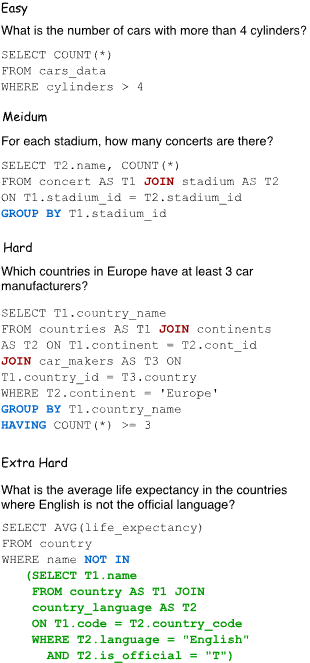
\includegraphics[width=0.35\textwidth]{image.png}
\caption{SQL query examples in 4 hardness levels. Credit: Spider [1]}
\label{fig:hardness-levels}
\end{figure}

\subsection{Prompting and Input}
\label{sec:prompting}

Each model receives three pieces of information in a single zero-shot user turn: a system instruction explaining its role as a Text-to-SQL generator, the database schema (table names, column names, primary keys, and foreign-key relationships, with no example rows), and the natural-language question. No few-shot examples are provided, so that the experiment measures each model's ability to generate SQL from instructions and schema information alone, without the confound of examples steering its output style. The prompt template is identical across all three models, so that differences in performance can be attributed to the models rather than to differences in prompting.

\textbf{Prompt template:}
\begin{verbatim}
Given the following SQLite database schema, write a SQL query that answers
the question.

{schema}

Question: {question}

Respond with only the SQL query in a ```sql code block.
\end{verbatim}

See \hyperref[sec:appendix1]{Appendix 1} for a worked example: a full schema, a question, and the resulting filled prompt.

\subsection{SQL Extraction}
\label{sec:sql-extraction}

For each sample, we decode the model's generated tokens into text using the model-specific tokenizer, and check for the presence of a \texttt{</think>} token. If \texttt{</think>} was generated, we take all text generated before \texttt{</think>} as the reasoning trace and all text to the right as the output SQL; DeepSeek-R1-Distill-Qwen-1.5B is the only model of the three that can emit this token. The SQL is then extracted from the first \texttt{```sql} code block in that remaining text. The extracted SQL is passed to the evaluation script as-is. Outputs that cannot be extracted or parsed are counted as incorrect on every metric rather than excluded from the evaluation, as unusable output is a task failure (see \ref{sec:evaluation-metrics} and \ref{sec:invalid-outputs}).

\subsection{Inference Settings}
\label{sec:inference-settings}

All models are evaluated using the same decoding configuration: greedy decoding (temperature and top-p are not applicable) for consistent, reproducible results between runs. The maximum output length differs by model: 256 tokens for Qwen3-0.6B, and 4096 tokens for both Qwen3-4B and DeepSeek-R1-Distill-Qwen-1.5B. For DeepSeek, the larger budget is needed because its output also has to contain a full reasoning trace rather than only the SQL query; Qwen3-4B is given the same, larger budget as DeepSeek so that a tighter token limit can be ruled out as the reason for any difference between them on invalid-output rate (\ref{sec:invalid-outputs}) or inference time (\ref{sec:efficiency}). Qwen3-0.6B and Qwen3-4B are both run with thinking mode off (both support it). DeepSeek-R1-Distill-Qwen-1.5B always produces a reasoning trace and has no documented way to disable thinking mode, so it is evaluated as the reasoning condition against the two non-reasoning Qwen3 models. All inference runs on the same 1x RTX 4090 GPU described in \ref{sec:models}, with batch size 1.

\subsection{Evaluation}
\label{sec:evaluation-metrics}

We evaluate the output using the same metrics as the Spider paper [1]. These are:

\begin{enumerate}
\item Component Matching
    \begin{itemize}
        \item For each of the following components:
        \begin{itemize}
            \item SELECT
            \item WHERE
            \item GROUP BY
            \item ORDER BY
            \item KEYWORDS (including all SQL keywords without column names and operators)
        \end{itemize}
        \item Decompose each component in the prediction and ground truth as bags of several sub-components and check whether or not these two sets of components match completely.
        \item Checks accuracy, recall, and F1
    \end{itemize}
\item Exact Matching Accuracy
    \begin{itemize}
        \item We measure whether the generated query as a whole is equivalent to the last section
        \item The generated query is correct only if all components are correct
        \item Checks only accuracy
    \end{itemize}
\item Execution Accuracy
    \begin{itemize}
        \item A list of gold values for each question is given
        \item We measure how many gold values the generated query extracts when executed
        \item Checks only accuracy
    \end{itemize}
\end{enumerate}

If output is invalid or unparsable, then it fails all 3 dimensions (component matching, exact matching, execution accuracy), consistent with how \ref{sec:sql-extraction} extracts and passes SQL to this evaluation script. This is reasonable as invalid/unparsable output cannot be applied to SQL and thus must be avoided and penalized heavily; Results~\ref{sec:invalid-outputs} reports how often this happens for each model.

\section{Task 1 -- RQ1: Results}
\label{sec:rq1-results}

\subsection{Overall Model Performance}
\label{sec:overall-performance}

Below we report how Qwen3-0.6B, Qwen3-4B, and Deepseek-R1-Distill-Qwen3-1.5B perform on the Spider benchmark across all 3 metrics (Component Matching, Exact Matching Accuracy, Execution Accuracy). We calculate the values per problem difficulty as well as overall, and display them in the below tables.

\begin{table}[H]
\centering
\footnotesize
\caption{Overall performance summary, aggregated across all difficulties (all 1034 problems). Component matching is accuracy / recall / F1 (macro-averaged, see the note on table~\ref{tab:difficulty-component} in \ref{sec:rq1-interpretation}). Per-difficulty breakdowns are in tables~\ref{tab:difficulty-component}--\ref{tab:difficulty-execution}.}
\label{tab:overall-performance}
\resizebox{\textwidth}{!}{%
\begin{tabular}{lllccc}
\toprule
Model & Parameters & Category & Component matching & Exact matching & Execution accuracy \\
\midrule
Qwen3-0.6B & 0.6B & Decoder-only & 0.628 / 0.209 / 0.314 & 0.099 & 0.209 \\
Qwen3-4B & 4B & Decoder-only & 0.797 / 0.306 / 0.442 & 0.256 & 0.353 \\
DeepSeek-R1-Distill-Qwen-1.5B & 1.5B & Reasoning & 0.661 / 0.174 / 0.275 & 0.085 & 0.121 \\
\bottomrule
\end{tabular}}
\end{table}

All models are evaluated zero-shot with the same prompt on the 20 databases of the Spider dev set. Aggregated across all difficulties and databases, every model is still far from solving the task: execution accuracy ranges from 0.121 (DeepSeek) to 0.353 (Qwen3-4B) and exact matching accuracy from 0.085 (DeepSeek) to 0.256 (Qwen3-4B). Execution accuracy is higher than exact matching accuracy for all three models (for example 0.353 vs.\ 0.256 for Qwen3-4B), which suggests that at least some of the queries that return the correct result are written differently from the gold SQL (see \ref{sec:rq1-interpretation} for more on this relationship). Of the three models, Qwen3-4B is now the best on almost every metric, database, and difficulty level; \ref{sec:by-database} and \ref{sec:rq1-interpretation} quantify how consistently. Table~\ref{tab:inference-time} reports the efficiency side of this comparison: inference time per example.

\subsection{Performance by Query Difficulty}
\label{sec:by-difficulty}

\begin{table}[H]
\centering
\footnotesize
\caption{Component matching (accuracy / recall / F1) by difficulty.}
\label{tab:difficulty-component}
\begin{tabular}{lcc}
\toprule
Model & easy & medium \\
\midrule
Problems (n) & 248 & 446 \\
Qwen3-0.6B & 0.675 / 0.308 / 0.423 & 0.582 / 0.235 / 0.334 \\
Qwen3-4B & 0.838 / 0.574 / 0.681 & 0.670 / 0.306 / 0.420 \\
DeepSeek-R1-Distill-Qwen-1.5B & 0.566 / 0.288 / 0.382 & 0.642 / 0.185 / 0.287 \\
\bottomrule
\end{tabular}

\vspace{0.5em}

\begin{tabular}{lccc}
\toprule
Model & hard & extra & all \\
\midrule
Problems (n) & 174 & 166 & 1034 \\
Qwen3-0.6B & 0.540 / 0.141 / 0.223 & 0.578 / 0.160 / 0.250 & 0.628 / 0.209 / 0.314 \\
Qwen3-4B & 0.796 / 0.262 / 0.394 & 0.485 / 0.150 / 0.229 & 0.797 / 0.306 / 0.442 \\
DeepSeek-R1-Distill-Qwen-1.5B & 0.543 / 0.113 / 0.187 & 0.389 / 0.104 / 0.164 & 0.661 / 0.174 / 0.275 \\
\bottomrule
\end{tabular}
\end{table}

\begin{table}[H]
\centering
\footnotesize
\caption{Exact matching accuracy by difficulty.}
\label{tab:difficulty-exact}
\begin{tabular}{lccccc}
\toprule
Model & easy & medium & hard & extra & all \\
\midrule
Problems (n) & 248 & 446 & 174 & 166 & 1034 \\
Qwen3-0.6B & 0.157 & 0.137 & 0.006 & 0.006 & 0.099 \\
Qwen3-4B & 0.508 & 0.262 & 0.115 & 0.012 & 0.256 \\
DeepSeek-R1-Distill-Qwen-1.5B & 0.214 & 0.078 & 0.000 & 0.000 & 0.085 \\
\bottomrule
\end{tabular}
\end{table}

\begin{table}[H]
\centering
\footnotesize
\caption{Execution accuracy by difficulty.}
\label{tab:difficulty-execution}
\begin{tabular}{lccccc}
\toprule
Model & easy & medium & hard & extra & all \\
\midrule
Problems (n) & 248 & 446 & 174 & 166 & 1034 \\
Qwen3-0.6B & 0.210 & 0.276 & 0.126 & 0.114 & 0.209 \\
Qwen3-4B & 0.565 & 0.345 & 0.276 & 0.139 & 0.353 \\
DeepSeek-R1-Distill-Qwen-1.5B & 0.258 & 0.128 & 0.017 & 0.006 & 0.121 \\
\bottomrule
\end{tabular}
\end{table}

We break every metric down by the Spider Hardness Criteria (\ref{sec:eval-data}) as query difficulty is a first-order driver of Text-to-SQL performance; comparing models only in aggregate would hide whether a model's advantage holds up as queries get harder.

Performance decreases with difficulty for every model, but the decrease is steepest for Qwen3-0.6B and DeepSeek: their exact matching and execution accuracy are both at most 0.034 and 0.126 respectively on hard and extra problems, down from as high as 0.210-0.258 (easy execution) on the easiest problems (table~\ref{tab:difficulty-exact} and table~\ref{tab:difficulty-execution}). Qwen3-4B degrades on the same relative scale but from a much higher starting point, from 0.508 easy exact matching / 0.565 easy execution accuracy down to 0.012 extra exact matching / 0.139 extra execution accuracy. Despite the degredation, it remains the best of the three models at every single difficulty level on both metrics (tables~\ref{tab:difficulty-exact}--\ref{tab:difficulty-execution}).

\subsection{Performance by Database}
\label{sec:by-database}

We also break execution and exact matching accuracy down by each of the 20 Spider dev databases. Qwen3-4B has the highest execution accuracy on 17 of the 20 databases outright (plus a tie on one more) and the highest exact matching accuracy on 18 of 20, while DeepSeek-R1-Distill-Qwen-1.5B is never highest on either metric; Qwen3-0.6B wins outright only on orchestra and battle\_death. Databases with few problems (real\_estate\_properties with n=4, voter\_1 with n=15, battle\_death with n=16, and museum\_visit with n=18) are too small to rank the models reliably, since a single problem changes a score by 6 to 25 percentage points. Execution accuracy ranges from 0.10 (course\_teach) to 0.53 (singer) for Qwen3-0.6B, from 0.19 (battle\_death) to 0.60 (singer) for Qwen3-4B, and from 0.00 (concert\_singer) to 0.27 (singer and voter\_1) for DeepSeek-R1-Distill-Qwen-1.5B (\hyperref[tab:db-execution]{Table 5}). The pattern on exact matching accuracy is just as one-sided (\hyperref[tab:db-exact]{Table 6}): Qwen3-4B is highest on 18 of 20 databases, ties Qwen3-0.6B on orchestra, and loses only on battle\_death; DeepSeek's exact matching accuracy is never the highest of the three, coming closest on flight\_2 (0.200 vs.\ Qwen3-4B's 0.350 and Qwen3-0.6B's 0.075). The full per-database tables and discussion are in \hyperref[sec:appendix2]{Appendix 2}.

\subsection{Invalid and Unparseable Outputs}
\label{sec:invalid-outputs}

We also count how often each model's output cannot be used as SQL at all: it either never produces a usable query within the token budget (\ref{sec:inference-settings}) or is truncated before finishing one. Per \ref{sec:evaluation-metrics}, these count as failures on every metric rather than being excluded, and this is a direct measure of how reliably each model follows the ``respond with only a SQL query'' instruction, independent of whether the SQL it does produce is correct. Qwen3-0.6B's invalid rate is 2.2\%, Qwen3-4B's is 0.0\%, and DeepSeek-R1-Distill-Qwen-1.5B's is 9.7\%, about 4x higher than Qwen3-0.6B's despite having the same 4096-token budget as Qwen3-4B (\ref{sec:inference-settings}), i.e. a larger token budget did not cause Qwen3-4B to run on or produce unusable output the way it does for DeepSeek. \ref{sec:rq1-interpretation} breaks DeepSeek's failures down further by difficulty and by why the generation failed (tables~\ref{tab:deepseek-outcome}--\ref{tab:deepseek-unfinished-by-difficulty}).

\subsection{Efficiency Measures}
\label{sec:efficiency}

\begin{table}[H]
\centering
\footnotesize
\caption{Output tokens per example}
\label{tab:tokens-per-example}
\begin{tabular}{lccccc}
\toprule
Model & easy & medium & hard & extra & all \\
\midrule
Qwen3-0.6B & 27.5 & 44.7 & 53.7 & 69.9 & 46.1 \\
Qwen3-4B & 23.6 & 37.3 & 46.2 & 59.0 & 39.0 \\
DeepSeek-R1-Distill-Qwen-1.5B & 610.8 & 768.4 & 1096.0 & 1176.9 & 851.3 \\
\bottomrule
\end{tabular}
\end{table}

Inference time is measured from the start of generation to the complete batch output, per batch of 1 example, excluding tokenization, model loading, and warm-up.

\begin{table}[H]
\centering
\footnotesize
\caption{Inference time.}
\label{tab:inference-time}
\begin{tabular}{lcc}
\toprule
Model & Total wall time (s) & Avg.\ time per example (s) \\
\midrule
Qwen3-0.6B & 123.9 & 0.120 \\
Qwen3-4B & 109.1 & 0.106 \\
DeepSeek-R1-Distill-Qwen-1.5B & 3059.8 & 2.959 \\
\bottomrule
\end{tabular}
\end{table}

DeepSeek is about 25x slower per example than Qwen3-0.6B and 28x slower than Qwen3-4B, consistent with its much higher average token count (table~\ref{tab:tokens-per-example}). Qwen3-4B, despite having about 7x as many parameters as Qwen3-0.6B, is marginally faster per example (0.106s vs.\ 0.120s), consistent with it generating fewer tokens on average (39.0 vs.\ 46.1, table~\ref{tab:tokens-per-example}) despite having the same 16x larger token budget as DeepSeek (\ref{sec:inference-settings}).

\begin{table}[H]
\centering
\footnotesize
\caption{DeepSeek-R1-Distill-Qwen-1.5B by generation outcome. ``Cut'' means the generation reached the 4096-token limit.}
\label{tab:deepseek-outcome}
\begin{tabular}{lccccc}
\toprule
Outcome & Problems (n) & Share & Avg.\ tokens & Exact match & Component F1 \\
\midrule
Finished with SQL & 934 & 90.3\% & 512 & 0.094 & 0.286 \\
Finished, no usable SQL & 2 & 0.2\% & 284 & 0.000 & 0.100 \\
Cut while answering (after \texttt{</think>}) & 13 & 1.3\% & 4096 & 0.000 & 0.096 \\
Cut while thinking (no \texttt{</think>}) & 85 & 8.2\% & 4096 & 0.000 & 0.093 \\
All & 1034 & 100\% & 851 & 0.085 & 0.275 \\
\bottomrule
\end{tabular}
\end{table}

\begin{table}[H]
\centering
\footnotesize
\caption{The same 934 questions that DeepSeek finished, for all three models.}
\label{tab:deepseek-finished-934}
\begin{tabular}{lcc}
\toprule
Model & Exact match & Component F1 \\
\midrule
DeepSeek-R1-Distill-Qwen-1.5B & 0.094 & 0.286 \\
Qwen3-0.6B & 0.103 & 0.317 \\
Qwen3-4B & 0.257 & 0.440 \\
\bottomrule
\end{tabular}
\end{table}

\begin{table}[H]
\centering
\footnotesize
\caption{Are the cut-off DeepSeek generations infinite self-repetition loops? A text that repeats itself compresses well, so a low compression ratio of the last 3000 characters indicates a loop.}
\label{tab:deepseek-repetition}
\begin{tabular}{lcccc}
\toprule
Generations & n & Median compression ratio & Ratio $<$ 0.15 & Last 150 characters repeat 3 or more times \\
\midrule
Cut off & 98 & 0.095 & 95.9\% & 96.9\% \\
Finished & 936 & 0.418 & 0.0\% & 0.2\% \\
\bottomrule
\end{tabular}
\end{table}

\begin{table}[H]
\centering
\footnotesize
\caption{Share of DeepSeek generations that did not finish with SQL, by difficulty.}
\label{tab:deepseek-unfinished-by-difficulty}
\begin{tabular}{lccccc}
\toprule
 & easy & medium & hard & extra & all \\
\midrule
Problems (n) & 248 & 446 & 174 & 166 & 1034 \\
Not finished with SQL (n) & 15 & 33 & 25 & 27 & 100 \\
Share & 6.0\% & 7.4\% & 14.4\% & 16.3\% & 9.7\% \\
\bottomrule
\end{tabular}
\end{table}

\section{Interpretation and Answer to Research Question (RQ1)}
\label{sec:rq1-interpretation}

\textbf{RQ1:} How do (selected) LLMs perform on cross-domain Text-to-SQL?

\vspace{10px}

All three models are still far from solving the task in this zero-shot setting: exact matching accuracy ranges from 0.085 to 0.256 and execution accuracy from 0.121 to 0.353 (table~\ref{tab:overall-performance}). Difficulty and database effects are discussed in \ref{sec:by-difficulty} and \ref{sec:by-database}; here we interpret the effects of model size and reasoning architecture and the exact-match/execution-accuracy relationship, and state the answer to RQ1 as three findings.

\textbf{First, within the Qwen family, scale is a strong and almost uniform predictor of performance, but an intermediate-size reasoning model from the Deepseek family still loses to the smallest model in the Qwen family.} Aggregated across all difficulties, Qwen3-4B has the best component matching (0.797 / 0.306 / 0.442), exact matching (0.256), and execution accuracy (0.353) of the three (table~\ref{tab:overall-performance}), and it beats Qwen3-0.6B on exact matching and execution accuracy at every individual difficulty level, including hard (0.115 vs.\ 0.006) and extra (0.012 vs.\ 0.006), where the smaller model solves almost nothing (tables~\ref{tab:difficulty-exact}--\ref{tab:difficulty-execution}). This is the largest, most consistent effect in the RQ1 results. The one exception is component matching on extra-hard problems, where Qwen3-0.6B's accuracy, recall, and F1 (0.578 / 0.160 / 0.250) are all slightly higher than Qwen3-4B's (0.485 / 0.150 / 0.229), the only point in the RQ1 results where the smaller Qwen3 model wins outright (table~\ref{tab:difficulty-component}). DeepSeek-R1-Distill-Qwen-1.5B sits between the two Qwen3 models in parameter count (1.5B) and is the only one that reasons, yet it is the lowest of the three on every aggregate metric (0.275 component F1, 0.085 exact matching, 0.121 execution accuracy) except its own component-matching accuracy (0.661 vs.\ 0.628 for Qwen3-0.6B). Thus, scale predicts performance well within a family, but does not transfer across the reasoning/non-reasoning boundary: having more parameters than Qwen3-0.6B did not help DeepSeek catch up to it.

\textbf{Second, the reasoning architecture itself, not parameter count, is the main driver of DeepSeek's low score.} Its invalid-output rate (9.7\%) is markedly higher than Qwen3-0.6B's (2.2\%) and Qwen3-4B's (0.0\% in this run) (\ref{sec:invalid-outputs}). In tables~\ref{tab:deepseek-outcome}--\ref{tab:deepseek-unfinished-by-difficulty}, 100 of 1034 generations (9.7\%) end without usable SQL. 85 never leave the reasoning phase, 13 are cut while writing the answer, and 2 finish without SQL. The number of unusable SQL generations also grows with difficulty, from 6.0\% on easy to 16.3\% on extra problems. These are not cases of long productive reasoning either: 95.9\% of the cut-off generations are highly self-repetitive (compression ratio below 0.15, median compression ratio 0.095, vs.\ 0.418 for finished generations), rewriting the same query and repeating phrases like ``So the final query is:'' without converging. Finishing does not make it better either: on the 934 questions DeepSeek does finish, its exact matching (0.094) and component F1 (0.286) are still below Qwen3-0.6B's on the same questions (0.103 / 0.317) and far below Qwen3-4B's (0.257 / 0.440), despite generating 512 tokens per question on average there, against 46 and 39 tokens overall for Qwen3-0.6B and Qwen3-4B (about 18x and 22x fewer). This extra length also costs time: DeepSeek is 25-28x slower per example than either Qwen3 model (\ref{sec:efficiency}). The reasoning trace mostly lengthens the output and sometimes never terminates, without improving the SQL when it does, and size alone is not the explanation, since Qwen3-4B is both bigger than DeepSeek and the best model in the comparison. Thus, reasoning architecture itself, not the parameter count, is the main driver of DeepSeek's low score.

\textbf{Third, query difficulty has a substantial, consistent effect on every model, including the best one.} Exact matching and execution accuracy both fall sharply from easy to extra-hard problems for all three models (\ref{sec:by-difficulty}). Qwen3-4B's drop is from a much higher base (0.508 to 0.012 exact matching, 0.565 to 0.139 execution accuracy) and it remains the best model at every difficulty level on both metrics, but the drop itself is just as steep in relative terms as for the other two models, and the hardest problems remain largely unsolved even for it.

\textbf{Exact match vs.\ execution accuracy.} For all three models, execution accuracy aggregated across all difficulties exceeds exact matching accuracy (table~\ref{tab:overall-performance}): 0.209 vs.\ 0.099 for Qwen3-0.6B, 0.353 vs.\ 0.256 for Qwen3-4B, and 0.121 vs.\ 0.085 for DeepSeek. Since exact matching requires every SQL component to match the gold query while execution accuracy only requires the same result set, this gap indicates each model writes some queries that are valid and correct but phrased differently from the gold SQL (e.g.\ a different but equivalent join order, or an explicit column list where the gold query uses \texttt{SELECT *}). The gap is widest for Qwen3-0.6B (11.0 points), close behind for Qwen3-4B (9.7 points), and narrowest for DeepSeek (3.6 points); DeepSeek's narrower gap reflects it producing fewer alternative-but-valid queries. Qwen3-4B's gap is almost as wide as Qwen3-0.6B's despite much higher absolute accuracy, so scaling up within the Qwen3 family raises both Exact Match Accuracy and Execution Accuracy together rather than closing the gap between them.

\textbf{Limitations.} Our working hypothesis is that Text-to-SQL at this scale does not benefit from an explicit reasoning trace, and that a non-reasoning model is sufficient, with performance instead scaling with parameter count within a fixed model family. The results are consistent with this hypothesis. However, they do not establish that Text-to-SQL is too simple for reasoning models in general due to several factors:

\begin{itemize}
\item \textbf{Truncation and failed outputs for DeepSeek.} These count as failures on every metric and lower its recall, exact matching, and execution scores, but table~\ref{tab:deepseek-finished-934} shows removing them would not change the ranking (DeepSeek is also lower on the questions it finished), and table~\ref{tab:deepseek-repetition} shows the cut-off generations are repetition loops, so a larger token budget is unlikely to rescue them.
\item \textbf{Model differences beyond reasoning.} Qwen3-0.6B and Qwen3-4B share a model family, isolating the effect of scale between them, but DeepSeek differs from both in family, size, and pretraining/post-training, not only in whether it reasons; it is also a distilled model, so the effect of reasoning cannot be fully separated from distillation quality.
\item \textbf{Aggregated component matching.} The component matching figures in table~\ref{tab:difficulty-component} (and in table~\ref{tab:overall-performance}) are our own macro-average (mean of the 10 per-component accuracy and recall scores, with F1 computed from these two means), not a number reported by Spider.
\end{itemize}

Overall, in this zero-shot, cross-domain setting, a larger non-reasoning decoder-only model (Qwen3-4B, 4B) clearly outperforms both a same-family model at under a sixth its size (Qwen3-0.6B) and a reasoning model of intermediate size from a different family (DeepSeek-R1-Distill-Qwen-1.5B, 1.5B), while also being faster per example than either. None of the three models solve more than half of even the easiest problems or more than a small fraction of hard or extra-hard queries. This answers RQ1 for the three models evaluated.
 into REPORT.tex in place of the current inline
% "Task 1 -- RQ1: Methodology & Results" / "Task 1 -- RQ1: Results" content.
% REPORT.tex already loads every package this fragment needs (booktabs, array,
% graphicx, float, caption, hyperref), so no extra preamble is required.
%
% Annotations made while converting this to reference-based numbering:
%  - All \subsection*{N.M ...} / \section*{...} became real, numbered
%    \section/\subsection commands with the leading "N.M" stripped from the
%    title text (LaTeX now generates it), each with a \label. The former
%    \subsection*{3. Interpretation...} is promoted to a top-level \section,
%    since it was already numbered as a peer of Parts 1 and 2, not a child
%    of Part 2.
%  - Every table/figure got a \label right after its \caption, and every
%    in-text "table 1", "tables 2-4", "2.2", "Appendix 2", etc. became a
%    \ref (or \hyperref for Appendix 2/3, which live outside this file --
%    see note below). Because the Models table (1.1) is now counted and the
%    Appendix 2/3 tables are not part of this file's sequential numbering,
%    the printed table numbers shift versus the pasted draft (e.g. "table 1"
%    -> Table 2, "table 8" -> Table 6); every mention uses \ref, so this is
%    self-consistent and will stay correct if tables move again.
%  - Fixed a leftover inconsistency in 1.5: the draft's 1.1 and 2.5 both
%    state batch size 1 (confirmed correct), but 1.5 still said "batch size
%    128" (leftover from an earlier draft) -- corrected to 1.
%  - Both TODOs in the pasted draft are resolved inline: 2.2 now cites
%    Tables 4-5 directly instead of a placeholder, and 2.3 now cites the
%    concrete per-database numbers from Appendix 2 (pulled from REPORT.tex's
%    existing Appendix 2 prose) instead of a placeholder.
%  - The Overall Performance table's caption promises "the note on table 2
%    in 3" (i.e. a note about macro-averaged component matching, to appear
%    in the Interpretation section), but the pasted draft's Limitations list
%    dropped that bullet (it only kept "Truncation" and "Model differences").
%    Restored the "Aggregated component matching" bullet from the prior
%    REPORT.tex draft so the caption's forward reference resolves to real
%    content; this is a content restoration, not just a labeling change,
%    so flagging it here. The other previously-present bullet ("Single run
%    and sample size") was NOT restored, since nothing in the new draft
%    points to it -- worth confirming with the author whether that drop was
%    intentional.
%  - Appendix 1/2/3 and their tables (5, 6, 7) live in REPORT.tex, outside
%    this file. REPORT.tex's appendix tables keep their existing manual
%    "Table 5/6/7:" caption numbering (renumbering them would require
%    restructuring the whole document's table order, which is out of scope
%    here); \label{tab:db-execution}, \label{tab:db-exact} and
%    \label{tab:invalid-outputs} were added to those tables in REPORT.tex
%    (additive only, no visible change) so this file can link to them.
%    Since their printed numbers are not auto-generated, this file links to
%    them with \hyperref[label]{5}-style calls (a real clickable link, with
%    text matching the manual number already in their caption) rather than
%    \ref (which would print whatever their true document-order table
%    number is, not 5/6/7).

\section{Task 1 -- RQ1: Methodology \& Results}
\label{sec:rq1-methods}

\textbf{RQ1:} How do (selected) LLMs perform on cross-domain Text-to-SQL?

In this report we evaluate the performance of decoder-only language models as well as reasoning LLMs on cross-domain SQL.

\subsection{Models}
\label{sec:models}

We compare two decoder-only LLMs from the same model family at different scales (Qwen3-0.6B and Qwen3-4B) against one reasoning LLM, so that the comparison isolates the effect of scale within a fixed family from the effect of an explicit reasoning trace, as much as a 3-model study can. All three are accessed as local inference over their bf16 Huggingface checkpoints on 1x NVIDIA GeForce RTX 4090 GPU (no API-based models), so that inference parameters are fully under our control (see \ref{sec:inference-settings}). We evaluate using batch sizes of 1.

\begin{table}[H]
\centering
\footnotesize
\caption{Models compared in RQ1.}
\label{tab:models}
\resizebox{\textwidth}{!}{%
\begin{tabular}{llllll}
\toprule
Model & Category & Parameters & Quantization & Access & Thinking mode \\
\midrule
Qwen3-0.6B [2] & Decoder-only & 0.6B & bf16 (none beyond release precision) & Local, Huggingface checkpoint & Disabled \\
Qwen3-4B [2] & Decoder-only & 4B & bf16 (none beyond release precision) & Local, Huggingface checkpoint & Disabled \\
DeepSeek-R1-Distill-Qwen-1.5B [4] & Reasoning & 1.5B & bf16 (none beyond release precision) & Local, Huggingface checkpoint & Always on (no disable option) \\
\bottomrule
\end{tabular}}
\end{table}

All three are dense (non-MoE) models, so no distinction between total and active parameters applies.

\subsection{Evaluation Data}
\label{sec:eval-data}

We use all 1034 examples in the Spider [1] development split, with no subsampling and therefore no sampling seed to report; every example is included, so the per-database counts below and the per-database results tables (\hyperref[tab:db-execution]{5} and \hyperref[tab:db-exact]{6}) enumerate exactly which examples are used. To evaluate cross-domain performance, we additionally report results separately for each of the 20 databases in the Spider dev set: world\_1 (120 problems), car\_1 (92), cre\_Doc\_Template\_Mgt (84), dog\_kennels (82), flight\_2 (80), student\_transcripts\_tracking (78), wta\_1 (62), tvshow (62), network\_1 (56), concert\_singer (45), pets\_1 (42), poker\_player (40), orchestra (40), employee\_hire\_evaluation (38), course\_teach (30), singer (30), museum\_visit (18), battle\_death (16), voter\_1 (15), and real\_estate\_properties (4).

We also use the Spider Hardness Criteria, where queries are assigned difficulties based on the number of SQL components, selections, and conditions, so that queries that contain more SQL keywords are considered harder.

\begin{figure}[H]
\centering
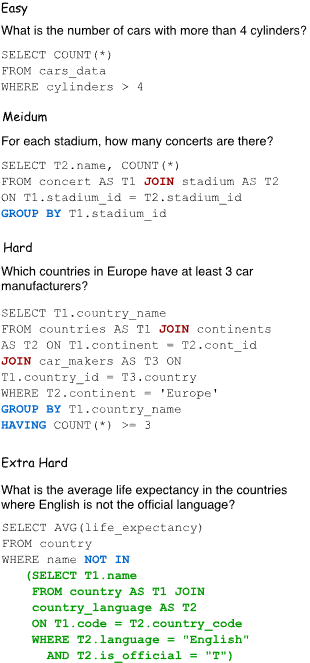
\includegraphics[width=0.35\textwidth]{image.png}
\caption{SQL query examples in 4 hardness levels. Credit: Spider [1]}
\label{fig:hardness-levels}
\end{figure}

\subsection{Prompting and Input}
\label{sec:prompting}

Each model receives three pieces of information in a single zero-shot user turn: a system instruction explaining its role as a Text-to-SQL generator, the database schema (table names, column names, primary keys, and foreign-key relationships, with no example rows), and the natural-language question. No few-shot examples are provided, so that the experiment measures each model's ability to generate SQL from instructions and schema information alone, without the confound of examples steering its output style. The prompt template is identical across all three models, so that differences in performance can be attributed to the models rather than to differences in prompting.

\textbf{Prompt template:}
\begin{verbatim}
Given the following SQLite database schema, write a SQL query that answers
the question.

{schema}

Question: {question}

Respond with only the SQL query in a ```sql code block.
\end{verbatim}

See \hyperref[sec:appendix1]{Appendix 1} for a worked example: a full schema, a question, and the resulting filled prompt.

\subsection{SQL Extraction}
\label{sec:sql-extraction}

For each sample, we decode the model's generated tokens into text using the model-specific tokenizer, and check for the presence of a \texttt{</think>} token. If \texttt{</think>} was generated, we take all text generated before \texttt{</think>} as the reasoning trace and all text to the right as the output SQL; DeepSeek-R1-Distill-Qwen-1.5B is the only model of the three that can emit this token. The SQL is then extracted from the first \texttt{```sql} code block in that remaining text. The extracted SQL is passed to the evaluation script as-is. Outputs that cannot be extracted or parsed are counted as incorrect on every metric rather than excluded from the evaluation, as unusable output is a task failure (see \ref{sec:evaluation-metrics} and \ref{sec:invalid-outputs}).

\subsection{Inference Settings}
\label{sec:inference-settings}

All models are evaluated using the same decoding configuration: greedy decoding (temperature and top-p are not applicable) for consistent, reproducible results between runs. The maximum output length differs by model: 256 tokens for Qwen3-0.6B, and 4096 tokens for both Qwen3-4B and DeepSeek-R1-Distill-Qwen-1.5B. For DeepSeek, the larger budget is needed because its output also has to contain a full reasoning trace rather than only the SQL query; Qwen3-4B is given the same, larger budget as DeepSeek so that a tighter token limit can be ruled out as the reason for any difference between them on invalid-output rate (\ref{sec:invalid-outputs}) or inference time (\ref{sec:efficiency}). Qwen3-0.6B and Qwen3-4B are both run with thinking mode off (both support it). DeepSeek-R1-Distill-Qwen-1.5B always produces a reasoning trace and has no documented way to disable thinking mode, so it is evaluated as the reasoning condition against the two non-reasoning Qwen3 models. All inference runs on the same 1x RTX 4090 GPU described in \ref{sec:models}, with batch size 1.

\subsection{Evaluation}
\label{sec:evaluation-metrics}

We evaluate the output using the same metrics as the Spider paper [1]. These are:

\begin{enumerate}
\item Component Matching
    \begin{itemize}
        \item For each of the following components:
        \begin{itemize}
            \item SELECT
            \item WHERE
            \item GROUP BY
            \item ORDER BY
            \item KEYWORDS (including all SQL keywords without column names and operators)
        \end{itemize}
        \item Decompose each component in the prediction and ground truth as bags of several sub-components and check whether or not these two sets of components match completely.
        \item Checks accuracy, recall, and F1
    \end{itemize}
\item Exact Matching Accuracy
    \begin{itemize}
        \item We measure whether the generated query as a whole is equivalent to the last section
        \item The generated query is correct only if all components are correct
        \item Checks only accuracy
    \end{itemize}
\item Execution Accuracy
    \begin{itemize}
        \item A list of gold values for each question is given
        \item We measure how many gold values the generated query extracts when executed
        \item Checks only accuracy
    \end{itemize}
\end{enumerate}

If output is invalid or unparsable, then it fails all 3 dimensions (component matching, exact matching, execution accuracy), consistent with how \ref{sec:sql-extraction} extracts and passes SQL to this evaluation script. This is reasonable as invalid/unparsable output cannot be applied to SQL and thus must be avoided and penalized heavily; Results~\ref{sec:invalid-outputs} reports how often this happens for each model.

\section{Task 1 -- RQ1: Results}
\label{sec:rq1-results}

\subsection{Overall Model Performance}
\label{sec:overall-performance}

Below we report how Qwen3-0.6B, Qwen3-4B, and Deepseek-R1-Distill-Qwen3-1.5B perform on the Spider benchmark across all 3 metrics (Component Matching, Exact Matching Accuracy, Execution Accuracy). We calculate the values per problem difficulty as well as overall, and display them in the below tables.

\begin{table}[H]
\centering
\footnotesize
\caption{Overall performance summary, aggregated across all difficulties (all 1034 problems). Component matching is accuracy / recall / F1 (macro-averaged, see the note on table~\ref{tab:difficulty-component} in \ref{sec:rq1-interpretation}). Per-difficulty breakdowns are in tables~\ref{tab:difficulty-component}--\ref{tab:difficulty-execution}.}
\label{tab:overall-performance}
\resizebox{\textwidth}{!}{%
\begin{tabular}{lllccc}
\toprule
Model & Parameters & Category & Component matching & Exact matching & Execution accuracy \\
\midrule
Qwen3-0.6B & 0.6B & Decoder-only & 0.628 / 0.209 / 0.314 & 0.099 & 0.209 \\
Qwen3-4B & 4B & Decoder-only & 0.797 / 0.306 / 0.442 & 0.256 & 0.353 \\
DeepSeek-R1-Distill-Qwen-1.5B & 1.5B & Reasoning & 0.661 / 0.174 / 0.275 & 0.085 & 0.121 \\
\bottomrule
\end{tabular}}
\end{table}

All models are evaluated zero-shot with the same prompt on the 20 databases of the Spider dev set. Aggregated across all difficulties and databases, every model is still far from solving the task: execution accuracy ranges from 0.121 (DeepSeek) to 0.353 (Qwen3-4B) and exact matching accuracy from 0.085 (DeepSeek) to 0.256 (Qwen3-4B). Execution accuracy is higher than exact matching accuracy for all three models (for example 0.353 vs.\ 0.256 for Qwen3-4B), which suggests that at least some of the queries that return the correct result are written differently from the gold SQL (see \ref{sec:rq1-interpretation} for more on this relationship). Of the three models, Qwen3-4B is now the best on almost every metric, database, and difficulty level; \ref{sec:by-database} and \ref{sec:rq1-interpretation} quantify how consistently. Table~\ref{tab:inference-time} reports the efficiency side of this comparison: inference time per example.

\subsection{Performance by Query Difficulty}
\label{sec:by-difficulty}

\begin{table}[H]
\centering
\footnotesize
\caption{Component matching (accuracy / recall / F1) by difficulty.}
\label{tab:difficulty-component}
\begin{tabular}{lcc}
\toprule
Model & easy & medium \\
\midrule
Problems (n) & 248 & 446 \\
Qwen3-0.6B & 0.675 / 0.308 / 0.423 & 0.582 / 0.235 / 0.334 \\
Qwen3-4B & 0.838 / 0.574 / 0.681 & 0.670 / 0.306 / 0.420 \\
DeepSeek-R1-Distill-Qwen-1.5B & 0.566 / 0.288 / 0.382 & 0.642 / 0.185 / 0.287 \\
\bottomrule
\end{tabular}

\vspace{0.5em}

\begin{tabular}{lccc}
\toprule
Model & hard & extra & all \\
\midrule
Problems (n) & 174 & 166 & 1034 \\
Qwen3-0.6B & 0.540 / 0.141 / 0.223 & 0.578 / 0.160 / 0.250 & 0.628 / 0.209 / 0.314 \\
Qwen3-4B & 0.796 / 0.262 / 0.394 & 0.485 / 0.150 / 0.229 & 0.797 / 0.306 / 0.442 \\
DeepSeek-R1-Distill-Qwen-1.5B & 0.543 / 0.113 / 0.187 & 0.389 / 0.104 / 0.164 & 0.661 / 0.174 / 0.275 \\
\bottomrule
\end{tabular}
\end{table}

\begin{table}[H]
\centering
\footnotesize
\caption{Exact matching accuracy by difficulty.}
\label{tab:difficulty-exact}
\begin{tabular}{lccccc}
\toprule
Model & easy & medium & hard & extra & all \\
\midrule
Problems (n) & 248 & 446 & 174 & 166 & 1034 \\
Qwen3-0.6B & 0.157 & 0.137 & 0.006 & 0.006 & 0.099 \\
Qwen3-4B & 0.508 & 0.262 & 0.115 & 0.012 & 0.256 \\
DeepSeek-R1-Distill-Qwen-1.5B & 0.214 & 0.078 & 0.000 & 0.000 & 0.085 \\
\bottomrule
\end{tabular}
\end{table}

\begin{table}[H]
\centering
\footnotesize
\caption{Execution accuracy by difficulty.}
\label{tab:difficulty-execution}
\begin{tabular}{lccccc}
\toprule
Model & easy & medium & hard & extra & all \\
\midrule
Problems (n) & 248 & 446 & 174 & 166 & 1034 \\
Qwen3-0.6B & 0.210 & 0.276 & 0.126 & 0.114 & 0.209 \\
Qwen3-4B & 0.565 & 0.345 & 0.276 & 0.139 & 0.353 \\
DeepSeek-R1-Distill-Qwen-1.5B & 0.258 & 0.128 & 0.017 & 0.006 & 0.121 \\
\bottomrule
\end{tabular}
\end{table}

We break every metric down by the Spider Hardness Criteria (\ref{sec:eval-data}) as query difficulty is a first-order driver of Text-to-SQL performance; comparing models only in aggregate would hide whether a model's advantage holds up as queries get harder.

Performance decreases with difficulty for every model, but the decrease is steepest for Qwen3-0.6B and DeepSeek: their exact matching and execution accuracy are both at most 0.034 and 0.126 respectively on hard and extra problems, down from as high as 0.210-0.258 (easy execution) on the easiest problems (table~\ref{tab:difficulty-exact} and table~\ref{tab:difficulty-execution}). Qwen3-4B degrades on the same relative scale but from a much higher starting point, from 0.508 easy exact matching / 0.565 easy execution accuracy down to 0.012 extra exact matching / 0.139 extra execution accuracy. Despite the degredation, it remains the best of the three models at every single difficulty level on both metrics (tables~\ref{tab:difficulty-exact}--\ref{tab:difficulty-execution}).

\subsection{Performance by Database}
\label{sec:by-database}

We also break execution and exact matching accuracy down by each of the 20 Spider dev databases. Qwen3-4B has the highest execution accuracy on 17 of the 20 databases outright (plus a tie on one more) and the highest exact matching accuracy on 18 of 20, while DeepSeek-R1-Distill-Qwen-1.5B is never highest on either metric; Qwen3-0.6B wins outright only on orchestra and battle\_death. Databases with few problems (real\_estate\_properties with n=4, voter\_1 with n=15, battle\_death with n=16, and museum\_visit with n=18) are too small to rank the models reliably, since a single problem changes a score by 6 to 25 percentage points. Execution accuracy ranges from 0.10 (course\_teach) to 0.53 (singer) for Qwen3-0.6B, from 0.19 (battle\_death) to 0.60 (singer) for Qwen3-4B, and from 0.00 (concert\_singer) to 0.27 (singer and voter\_1) for DeepSeek-R1-Distill-Qwen-1.5B (\hyperref[tab:db-execution]{Table 5}). The pattern on exact matching accuracy is just as one-sided (\hyperref[tab:db-exact]{Table 6}): Qwen3-4B is highest on 18 of 20 databases, ties Qwen3-0.6B on orchestra, and loses only on battle\_death; DeepSeek's exact matching accuracy is never the highest of the three, coming closest on flight\_2 (0.200 vs.\ Qwen3-4B's 0.350 and Qwen3-0.6B's 0.075). The full per-database tables and discussion are in \hyperref[sec:appendix2]{Appendix 2}.

\subsection{Invalid and Unparseable Outputs}
\label{sec:invalid-outputs}

We also count how often each model's output cannot be used as SQL at all: it either never produces a usable query within the token budget (\ref{sec:inference-settings}) or is truncated before finishing one. Per \ref{sec:evaluation-metrics}, these count as failures on every metric rather than being excluded, and this is a direct measure of how reliably each model follows the ``respond with only a SQL query'' instruction, independent of whether the SQL it does produce is correct. Qwen3-0.6B's invalid rate is 2.2\%, Qwen3-4B's is 0.0\%, and DeepSeek-R1-Distill-Qwen-1.5B's is 9.7\%, about 4x higher than Qwen3-0.6B's despite having the same 4096-token budget as Qwen3-4B (\ref{sec:inference-settings}), i.e. a larger token budget did not cause Qwen3-4B to run on or produce unusable output the way it does for DeepSeek. \ref{sec:rq1-interpretation} breaks DeepSeek's failures down further by difficulty and by why the generation failed (tables~\ref{tab:deepseek-outcome}--\ref{tab:deepseek-unfinished-by-difficulty}).

\subsection{Efficiency Measures}
\label{sec:efficiency}

\begin{table}[H]
\centering
\footnotesize
\caption{Output tokens per example}
\label{tab:tokens-per-example}
\begin{tabular}{lccccc}
\toprule
Model & easy & medium & hard & extra & all \\
\midrule
Qwen3-0.6B & 27.5 & 44.7 & 53.7 & 69.9 & 46.1 \\
Qwen3-4B & 23.6 & 37.3 & 46.2 & 59.0 & 39.0 \\
DeepSeek-R1-Distill-Qwen-1.5B & 610.8 & 768.4 & 1096.0 & 1176.9 & 851.3 \\
\bottomrule
\end{tabular}
\end{table}

Inference time is measured from the start of generation to the complete batch output, per batch of 1 example, excluding tokenization, model loading, and warm-up.

\begin{table}[H]
\centering
\footnotesize
\caption{Inference time.}
\label{tab:inference-time}
\begin{tabular}{lcc}
\toprule
Model & Total wall time (s) & Avg.\ time per example (s) \\
\midrule
Qwen3-0.6B & 123.9 & 0.120 \\
Qwen3-4B & 109.1 & 0.106 \\
DeepSeek-R1-Distill-Qwen-1.5B & 3059.8 & 2.959 \\
\bottomrule
\end{tabular}
\end{table}

DeepSeek is about 25x slower per example than Qwen3-0.6B and 28x slower than Qwen3-4B, consistent with its much higher average token count (table~\ref{tab:tokens-per-example}). Qwen3-4B, despite having about 7x as many parameters as Qwen3-0.6B, is marginally faster per example (0.106s vs.\ 0.120s), consistent with it generating fewer tokens on average (39.0 vs.\ 46.1, table~\ref{tab:tokens-per-example}) despite having the same 16x larger token budget as DeepSeek (\ref{sec:inference-settings}).

\begin{table}[H]
\centering
\footnotesize
\caption{DeepSeek-R1-Distill-Qwen-1.5B by generation outcome. ``Cut'' means the generation reached the 4096-token limit.}
\label{tab:deepseek-outcome}
\begin{tabular}{lccccc}
\toprule
Outcome & Problems (n) & Share & Avg.\ tokens & Exact match & Component F1 \\
\midrule
Finished with SQL & 934 & 90.3\% & 512 & 0.094 & 0.286 \\
Finished, no usable SQL & 2 & 0.2\% & 284 & 0.000 & 0.100 \\
Cut while answering (after \texttt{</think>}) & 13 & 1.3\% & 4096 & 0.000 & 0.096 \\
Cut while thinking (no \texttt{</think>}) & 85 & 8.2\% & 4096 & 0.000 & 0.093 \\
All & 1034 & 100\% & 851 & 0.085 & 0.275 \\
\bottomrule
\end{tabular}
\end{table}

\begin{table}[H]
\centering
\footnotesize
\caption{The same 934 questions that DeepSeek finished, for all three models.}
\label{tab:deepseek-finished-934}
\begin{tabular}{lcc}
\toprule
Model & Exact match & Component F1 \\
\midrule
DeepSeek-R1-Distill-Qwen-1.5B & 0.094 & 0.286 \\
Qwen3-0.6B & 0.103 & 0.317 \\
Qwen3-4B & 0.257 & 0.440 \\
\bottomrule
\end{tabular}
\end{table}

\begin{table}[H]
\centering
\footnotesize
\caption{Are the cut-off DeepSeek generations infinite self-repetition loops? A text that repeats itself compresses well, so a low compression ratio of the last 3000 characters indicates a loop.}
\label{tab:deepseek-repetition}
\begin{tabular}{lcccc}
\toprule
Generations & n & Median compression ratio & Ratio $<$ 0.15 & Last 150 characters repeat 3 or more times \\
\midrule
Cut off & 98 & 0.095 & 95.9\% & 96.9\% \\
Finished & 936 & 0.418 & 0.0\% & 0.2\% \\
\bottomrule
\end{tabular}
\end{table}

\begin{table}[H]
\centering
\footnotesize
\caption{Share of DeepSeek generations that did not finish with SQL, by difficulty.}
\label{tab:deepseek-unfinished-by-difficulty}
\begin{tabular}{lccccc}
\toprule
 & easy & medium & hard & extra & all \\
\midrule
Problems (n) & 248 & 446 & 174 & 166 & 1034 \\
Not finished with SQL (n) & 15 & 33 & 25 & 27 & 100 \\
Share & 6.0\% & 7.4\% & 14.4\% & 16.3\% & 9.7\% \\
\bottomrule
\end{tabular}
\end{table}

\section{Interpretation and Answer to Research Question (RQ1)}
\label{sec:rq1-interpretation}

\textbf{RQ1:} How do (selected) LLMs perform on cross-domain Text-to-SQL?

\vspace{10px}

All three models are still far from solving the task in this zero-shot setting: exact matching accuracy ranges from 0.085 to 0.256 and execution accuracy from 0.121 to 0.353 (table~\ref{tab:overall-performance}). Difficulty and database effects are discussed in \ref{sec:by-difficulty} and \ref{sec:by-database}; here we interpret the effects of model size and reasoning architecture and the exact-match/execution-accuracy relationship, and state the answer to RQ1 as three findings.

\textbf{First, within the Qwen family, scale is a strong and almost uniform predictor of performance, but an intermediate-size reasoning model from the Deepseek family still loses to the smallest model in the Qwen family.} Aggregated across all difficulties, Qwen3-4B has the best component matching (0.797 / 0.306 / 0.442), exact matching (0.256), and execution accuracy (0.353) of the three (table~\ref{tab:overall-performance}), and it beats Qwen3-0.6B on exact matching and execution accuracy at every individual difficulty level, including hard (0.115 vs.\ 0.006) and extra (0.012 vs.\ 0.006), where the smaller model solves almost nothing (tables~\ref{tab:difficulty-exact}--\ref{tab:difficulty-execution}). This is the largest, most consistent effect in the RQ1 results. The one exception is component matching on extra-hard problems, where Qwen3-0.6B's accuracy, recall, and F1 (0.578 / 0.160 / 0.250) are all slightly higher than Qwen3-4B's (0.485 / 0.150 / 0.229), the only point in the RQ1 results where the smaller Qwen3 model wins outright (table~\ref{tab:difficulty-component}). DeepSeek-R1-Distill-Qwen-1.5B sits between the two Qwen3 models in parameter count (1.5B) and is the only one that reasons, yet it is the lowest of the three on every aggregate metric (0.275 component F1, 0.085 exact matching, 0.121 execution accuracy) except its own component-matching accuracy (0.661 vs.\ 0.628 for Qwen3-0.6B). Thus, scale predicts performance well within a family, but does not transfer across the reasoning/non-reasoning boundary: having more parameters than Qwen3-0.6B did not help DeepSeek catch up to it.

\textbf{Second, the reasoning architecture itself, not parameter count, is the main driver of DeepSeek's low score.} Its invalid-output rate (9.7\%) is markedly higher than Qwen3-0.6B's (2.2\%) and Qwen3-4B's (0.0\% in this run) (\ref{sec:invalid-outputs}). In tables~\ref{tab:deepseek-outcome}--\ref{tab:deepseek-unfinished-by-difficulty}, 100 of 1034 generations (9.7\%) end without usable SQL. 85 never leave the reasoning phase, 13 are cut while writing the answer, and 2 finish without SQL. The number of unusable SQL generations also grows with difficulty, from 6.0\% on easy to 16.3\% on extra problems. These are not cases of long productive reasoning either: 95.9\% of the cut-off generations are highly self-repetitive (compression ratio below 0.15, median compression ratio 0.095, vs.\ 0.418 for finished generations), rewriting the same query and repeating phrases like ``So the final query is:'' without converging. Finishing does not make it better either: on the 934 questions DeepSeek does finish, its exact matching (0.094) and component F1 (0.286) are still below Qwen3-0.6B's on the same questions (0.103 / 0.317) and far below Qwen3-4B's (0.257 / 0.440), despite generating 512 tokens per question on average there, against 46 and 39 tokens overall for Qwen3-0.6B and Qwen3-4B (about 18x and 22x fewer). This extra length also costs time: DeepSeek is 25-28x slower per example than either Qwen3 model (\ref{sec:efficiency}). The reasoning trace mostly lengthens the output and sometimes never terminates, without improving the SQL when it does, and size alone is not the explanation, since Qwen3-4B is both bigger than DeepSeek and the best model in the comparison. Thus, reasoning architecture itself, not the parameter count, is the main driver of DeepSeek's low score.

\textbf{Third, query difficulty has a substantial, consistent effect on every model, including the best one.} Exact matching and execution accuracy both fall sharply from easy to extra-hard problems for all three models (\ref{sec:by-difficulty}). Qwen3-4B's drop is from a much higher base (0.508 to 0.012 exact matching, 0.565 to 0.139 execution accuracy) and it remains the best model at every difficulty level on both metrics, but the drop itself is just as steep in relative terms as for the other two models, and the hardest problems remain largely unsolved even for it.

\textbf{Exact match vs.\ execution accuracy.} For all three models, execution accuracy aggregated across all difficulties exceeds exact matching accuracy (table~\ref{tab:overall-performance}): 0.209 vs.\ 0.099 for Qwen3-0.6B, 0.353 vs.\ 0.256 for Qwen3-4B, and 0.121 vs.\ 0.085 for DeepSeek. Since exact matching requires every SQL component to match the gold query while execution accuracy only requires the same result set, this gap indicates each model writes some queries that are valid and correct but phrased differently from the gold SQL (e.g.\ a different but equivalent join order, or an explicit column list where the gold query uses \texttt{SELECT *}). The gap is widest for Qwen3-0.6B (11.0 points), close behind for Qwen3-4B (9.7 points), and narrowest for DeepSeek (3.6 points); DeepSeek's narrower gap reflects it producing fewer alternative-but-valid queries. Qwen3-4B's gap is almost as wide as Qwen3-0.6B's despite much higher absolute accuracy, so scaling up within the Qwen3 family raises both Exact Match Accuracy and Execution Accuracy together rather than closing the gap between them.

\textbf{Limitations.} Our working hypothesis is that Text-to-SQL at this scale does not benefit from an explicit reasoning trace, and that a non-reasoning model is sufficient, with performance instead scaling with parameter count within a fixed model family. The results are consistent with this hypothesis. However, they do not establish that Text-to-SQL is too simple for reasoning models in general due to several factors:

\begin{itemize}
\item \textbf{Truncation and failed outputs for DeepSeek.} These count as failures on every metric and lower its recall, exact matching, and execution scores, but table~\ref{tab:deepseek-finished-934} shows removing them would not change the ranking (DeepSeek is also lower on the questions it finished), and table~\ref{tab:deepseek-repetition} shows the cut-off generations are repetition loops, so a larger token budget is unlikely to rescue them.
\item \textbf{Model differences beyond reasoning.} Qwen3-0.6B and Qwen3-4B share a model family, isolating the effect of scale between them, but DeepSeek differs from both in family, size, and pretraining/post-training, not only in whether it reasons; it is also a distilled model, so the effect of reasoning cannot be fully separated from distillation quality.
\item \textbf{Aggregated component matching.} The component matching figures in table~\ref{tab:difficulty-component} (and in table~\ref{tab:overall-performance}) are our own macro-average (mean of the 10 per-component accuracy and recall scores, with F1 computed from these two means), not a number reported by Spider.
\end{itemize}

Overall, in this zero-shot, cross-domain setting, a larger non-reasoning decoder-only model (Qwen3-4B, 4B) clearly outperforms both a same-family model at under a sixth its size (Qwen3-0.6B) and a reasoning model of intermediate size from a different family (DeepSeek-R1-Distill-Qwen-1.5B, 1.5B), while also being faster per example than either. None of the three models solve more than half of even the easiest problems or more than a small fraction of hard or extra-hard queries. This answers RQ1 for the three models evaluated.
 (this
% file links back into Task 1's tab:overall-performance and sec:rq1-results
% labels).
%
% Annotations made while converting this to reference-based numbering:
%  - \section*{Task 3 -- RQ3: Methodology}, \section*{Task 3 -- RQ3:
%    Results}, and \subsection*{Task 3 -- RQ3: Extension to Qwen3-4B} became
%    real, numbered \section/\subsection commands with \label. The
%    Extension subsection's title had "Task 3 -- RQ3: " stripped, since
%    that's now implied by nesting under the numbered Task 3 section
%    (matching how RQ1.tex strips the old manual "1.1"/"2.2" prefixes).
%  - Tables 16, 17, 18, 21, 22, 23, 24 each got a \label; every in-text
%    "Table 16/17/18/21/22/24" mention, including the forward reference
%    from Table 16's own caption to Table 18, became a \ref.
%  - Mentions of "Task 1" results now link to RQ1.tex's own labels
%    (sec:rq1-results, tab:overall-performance) via \hyperref, so they stay
%    live links even though Task 1's own numbering changed when RQ1.tex was
%    built.
%  - PRE-EXISTING ISSUE, NOT INTRODUCED HERE: Table 23's caption says
%    "Settings as in Table 19", and the "Longer training and
%    hyperparameters" paragraph discusses a 0.6B long-training sweep
%    (h0/h4/h5/h6, "the best long 0.6B run (0.613 / 0.632)") that has no
%    corresponding table anywhere in this document -- there is no Table 19
%    or Table 20 to point to. This looks like a 0.6B sweep table (the
%    equivalent of Table 23 for 0.6B) was planned/removed but the reference
%    to it was never updated. Left as plain, unlinked text "Table 19" since
%    there's nothing real to \ref; flagging for the author to either add
%    the missing table or fix the caption.

\section{Task 3 -- RQ3: Methodology}
\label{sec:rq3-methodology}

\textbf{RQ3:} To what extent does PlanPlay-SQL improve Qwen3-0.6B?

We improve Qwen3-0.6B [2] with thinking disabled, the same configuration as in \hyperref[sec:rq1-results]{Task 1}. We chose it because our compute is limited to a single RTX 4090, and iterative training on DeepSeek-R1-Distill-Qwen-1.5B would mean sampling and training on traces of about 850 tokens per question. Qwen3-0.6B generates about 46 tokens per question, so we can sample and train over the whole Spider training split. It also looked promising in Task 1, with the highest execution accuracy (0.209) and the shortest outputs. Task 1's execution accuracy is measured on schema-only databases (no rows), so it is not directly comparable to the mock-database execution accuracy reported for Task 3 below; we re-evaluated the original model on the mock databases as well (table~\ref{tab:rq3-dev-results-06b}, ``Original (Task 1)'' row, 0.130) so that the Task 3 comparison between original and adapted models is apples-to-apples. We call our method \textbf{PlanPlay-SQL}: the model first writes a short \emph{plan}, then is trained by verified self-\emph{play}. It combines three ideas from recent work on small-model Text-to-SQL. From [7] and [6], the model writes a short plan (tables and joins, columns, filters, aggregation and ordering) before the SQL, which gives a model with no thinking mode a place to organize the schema. We then fine-tune on the Spider training split in three stages, following [5]. First, a supervised warm start on gold SQL. Second, verification-based iterative fine-tuning: the model answers training questions, we execute its SQL and the gold SQL, keep the answers with matching results as positives, and fine-tune on them. Third, self-play fine-tuning: using the logistic loss of SPIN [8], we train the best checkpoint to prefer a verified correct answer over an incorrect answer produced by the worst checkpoint. Training uses only the Spider training split, and checkpoints are selected on held-out training databases, so the dev set stays untouched and evaluation stays cross-domain. We skip [5]'s synthetic question generation because Spider already provides gold SQL to execute against.

We expect PlanPlay-SQL to improve performance in two ways. The warm start teaches the model Spider's schema conventions and output style, which should raise exact and execution accuracy most, since Task 1 showed that many of the model's outputs are valid SQL that differs from the gold query. The verification and self-play stages then train on the model's own execution-checked outputs, which should reduce its remaining execution errors. We expect most of the gain to come from the warm start. Paper [5] found that verification-based fine-tuning gave most of its gains and self-play only a further 0.6 to 0.8 points, on much larger models, so self-play may add little at 0.6B. To measure each part, we report five rows on the same dev set and metrics as \hyperref[sec:rq1-results]{Task 1}: the original solution, the plan prompt only, the warm start only, warm start plus verification fine-tuning, and the full PlanPlay-SQL.

Gold SQL has no plan annotation, so the warm-start target is generated, not written by hand: a rule-based parser reads each gold query's top-level clauses (FROM/JOIN, SELECT, WHERE, GROUP BY/ORDER BY/LIMIT, and any set operator) with a small regex-based SQL splitter and renders them into the five-line plan format shown in the prompt template below. The parser is deterministic and derived purely from the gold SQL text; no model or human writes these training-target plans.

All stages use LoRA adapters (rank 32, alpha 64) on top of the frozen base checkpoint, rather than full fine-tuning. Table~\ref{tab:rq3-training-settings} below gives the learning rate, epochs, batch size, and training-item counts actually used for each stage; all stages share seed 0 and the same 707-question, 20-database held-out validation set described in \ref{sec:rq3-results}. ``Samples per question'' (k) is the number of candidate SQL completions sampled per training question during verification-based and self-play fine-tuning, before the correctness filter is applied; the resulting training-item count after filtering is reported in the ``training items'' column, since not every sampled question yields a usable positive or preference pair.

\begin{table}[H]
\centering
\footnotesize
\caption{Training settings for each stage in table~\ref{tab:rq3-validation-accuracy-06b}. Learning rate is the peak LR under a linear schedule.}
\label{tab:rq3-training-settings}
\resizebox{\textwidth}{!}{%
\begin{tabular}{lllccccc}
\toprule
Stage (table~\ref{tab:rq3-validation-accuracy-06b} row) & Init checkpoint & Training items & Samples/question (k) & Learning rate & Epochs & Batch size & Rounds \\
\midrule
Warm start (plan format, 1500 gold) & Qwen3-0.6B & 1500 gold SQL+plan pairs & --- & 2e-4 & 3 & 32 & 1 \\
+ 1500 further gold (supervised control) & Warm start & 1500 gold SQL+plan pairs & --- & 1e-4 & 1 & 32 & 1 \\
+ VBI-FT (same 1500 questions, hard only) & Warm start & 476 verified positives (of 1500 sampled) & 4 & 1e-4 & 1 & 32 & 1 \\
+ self-play, lower LR & VBI-FT (800-question round) & 279 verified preference pairs (of 800 sampled) & 4 & 1e-5 & 1 & 32 & 1 of 2 planned \\
+ self-play, higher LR & Warm start & 727 verified preference pairs (of 1500 sampled) & 4 & 1e-4 & 2 & 32 & 1 \\
\bottomrule
\end{tabular}}
\end{table}

\section{Task 3 -- RQ3: Results}
\label{sec:rq3-results}

Table~\ref{tab:rq3-dev-results-06b} compares the original Qwen3-0.6B from \hyperref[sec:rq1-results]{Task 1} with the adapted model on the same 1034 Spider dev questions, with the same metrics and the same execution-checking databases. The adapted model uses the plan-then-SQL prompt, greedy decoding, and a maximum of 384 new tokens (Task 1: 256). Execution accuracy is computed on mock databases (see the limitations below), so we treat exact matching accuracy as the more reliable number.

\begin{table}[H]
\centering
\footnotesize
\caption{Original and adapted Qwen3-0.6B on the Spider dev set, overall and by difficulty. Component matching is accuracy / recall / F1 (macro-averaged as in \hyperref[sec:rq1-interpretation]{Task 1}). Execution accuracy is on mock databases.}
\label{tab:rq3-dev-results-06b}
\resizebox{\textwidth}{!}{%
\begin{tabular}{llccccc}
\toprule
Metric & Model & easy & medium & hard & extra & all \\
\midrule
Problems (n) & & 248 & 446 & 174 & 166 & 1034 \\
Component matching & Original (Task 1) & 0.675 / 0.308 / 0.423 & 0.582 / 0.235 / 0.334 & 0.540 / 0.141 / 0.223 & 0.578 / 0.160 / 0.250 & 0.628 / 0.209 / 0.314 \\
 & Adapted & 0.809 / 0.763 / 0.786 & 0.750 / 0.643 / 0.693 & 0.815 / 0.626 / 0.708 & 0.696 / 0.478 / 0.567 & 0.783 / 0.636 / 0.702 \\
Exact matching & Original (Task 1) & 0.157 & 0.137 & 0.006 & 0.006 & 0.099 \\
 & Adapted & 0.762 & 0.594 & 0.385 & 0.265 & 0.546 \\
Execution (mock DB) & Original (Task 1) & 0.173 & 0.179 & 0.029 & 0.036 & 0.130 \\
 & Adapted & 0.794 & 0.583 & 0.443 & 0.277 & 0.561 \\
\bottomrule
\end{tabular}}
\end{table}

The adapted model is better on every metric and every difficulty level. Exact matching accuracy rises from 0.099 to 0.546 overall, and the largest relative gains are on hard (0.006 to 0.385) and extra (0.006 to 0.265) problems, which the original model almost never solved. Component matching recall rises from 0.209 to 0.636, so the model now writes most of the components the gold query contains. Execution accuracy on the mock databases rises from 0.130 to 0.561. The model is still weak on queries with set operations and nesting: the INTERSECT/UNION/EXCEPT and nested-query component (IUEN) has an accuracy of only 0.288. Our expectation that adapting on the Spider training split would help held, with much larger gains than we expected from a 0.6B model.

To see which part of the method helps, table~\ref{tab:rq3-validation-accuracy-06b} reports accuracy on a held-out validation set of 707 questions from 20 training databases that were never used for training. This validation set was used for choosing checkpoints, and the dev set was not.

\begin{table}[H]
\centering
\footnotesize
\caption{Validation accuracy (execution match on mock databases, 707 questions) after each stage. The row marked * uses a 300-question subset of the same validation set.}
\label{tab:rq3-validation-accuracy-06b}
\begin{tabular}{lc}
\toprule
Stage & Validation accuracy \\
\midrule
Base model, original prompt* & 0.407 \\
Base model, plan prompt, no training* & 0.050 \\
Warm start on 1500 gold questions (plan format) & 0.622 \\
+ 1500 further gold questions (supervised control) & 0.652 \\
+ VBI-FT on the same 1500 questions (no gold SQL, hard questions only, 476 verified samples) & 0.651 \\
+ self-play, lower learning rate (1e-5, 9 steps) & 0.631 \\
+ self-play, higher learning rate (1e-4, 46 steps) & 0.034 \\
\bottomrule
\end{tabular}
\end{table}

The warm start accounts for most of the gain (0.407 to 0.622). The plan prompt without training does very poorly (0.050), so the plan format only helps after fine-tuning. Verification-based fine-tuning matched the supervised control (0.651 vs.\ 0.652, a difference far smaller than the roughly 2-point sampling error of 707 questions) while using only 476 self-generated, execution-verified training items instead of 1500 gold ones and no gold SQL text. Self-play did not help: with a low learning rate it barely changed the model (0.622 to 0.631), and with a higher learning rate the training loss fell from 0.69 to 0.25 but accuracy collapsed to 0.034 with most outputs failing to execute. This matches the expectation from [5] that self-play adds little on top of verification-based fine-tuning, but it is more negative than the 0.6 to 0.8 points reported there. We report this as our final self-play result rather than rerunning with intermediate checkpointing and a lower learning rate: the lower-learning-rate run above already shows self-play adding at most 0.009 accuracy at this scale, so the higher-learning-rate collapse is a well-motivated negative finding about self-play's sensitivity on a 0.6B model, consistent with (and more pronounced than) [5]'s own small gains on larger models, rather than an open question that a rerun would likely overturn.

\textbf{Examples.} Out of 1034 dev questions, the adapted model gets 260 right that the original got wrong, loses 54 that the original got right, and both get 313 right (execution match on mock databases). One fixed example is the network\_1 question ``Show the student IDs and numbers of friends corresponding to each.'' The original model wrote \texttt{SELECT h.ID, h.name, h.grade, f.friend\_id FROM Highschooler h JOIN Friend f ON h.ID = f.student\_id}, which lists friends instead of counting them. The adapted model first wrote the plan \texttt{tables: friend; select: student\_id , count(*); group/order: group by student\_id} and then \texttt{SELECT student\_id , count(*) FROM friend GROUP BY student\_id}, which matches the gold query. One broken example is the tvshow question ``What are the titles of the cartoons sorted alphabetically?'' The original model wrote a correct query (\texttt{SELECT Title FROM Cartoon ORDER BY Title ASC}), but the adapted model's plan misspelled the table name (\texttt{tables: CARTON}), and the SQL that followed inherited the error (\texttt{SELECT Title FROM CARTON ORDER BY Title}), which fails to run. In this case the plan step propagated a mistake into the final query.

\textbf{Limitations.}

\begin{itemize}
\item \textbf{Mock databases.} The official Spider database files with rows were not available, so we generated databases with random rows seeded from the literals in each question's gold query. Execution accuracy on them only approximates the official execution accuracy. For example, Task 1's execution accuracy for the original model drops from 0.209 on schema-only databases to 0.130 on the mock databases (table~\ref{tab:overall-performance}), because on empty databases every query that returns nothing counts as correct. Exact matching accuracy does not depend on the databases.
\item \textbf{One run per configuration, one seed}, with no confidence intervals. The validation differences between the supervised control and VBI-FT are within sampling error.
\item \textbf{Different prompt and token budget.} The adapted model uses a different prompt and a larger token budget than the original, so the gain combines fine-tuning, the plan format, and the longer limit.
\item \textbf{Not the full method on dev.} The dev-set results are for the supervised stages only. VBI-FT and self-play were compared on the validation set.
\end{itemize}

\subsection{Extension to Qwen3-4B}
\label{sec:rq3-extension-4b}

To see whether PlanPlay-SQL still helps a larger model, we repeated the main RQ3 experiments on Qwen3-4B [2] with thinking disabled. Everything except the base checkpoint is unchanged: the same code (\texttt{--base Qwen/Qwen3-4B}), prompts, plan targets, LoRA target modules, training questions, seed, 707-question validation set, Spider dev set and mock databases, with one H100 per run. The ``Original'' row is our \hyperref[sec:rq1-results]{Task 1} greedy run of Qwen3-4B (thinking off), re-scored on the mock databases in the same way as the 0.6B baseline. We ran the table~\ref{tab:rq3-validation-accuracy-06b} stages with the table~\ref{tab:rq3-training-settings} settings and the four sweep settings that mattered for 0.6B (h0, h4, h5, h6). We did not re-run h1-h3, which were the weakest 0.6B settings. A 3-epoch warm start takes about 16 minutes on 4B, and a 30-epoch run on 3000 questions about 2 hours 10 minutes.

\begin{table}[H]
\centering
\footnotesize
\caption{Original and adapted Qwen3-4B on the Spider dev set (1034 questions). Adapted = plan-format warm start, 3 epochs (table~\ref{tab:rq3-training-settings} settings). Component matching is accuracy / recall / F1 as in table~\ref{tab:rq3-dev-results-06b}. Execution accuracy is on mock databases.}
\label{tab:rq3-dev-results-4b}
\resizebox{\textwidth}{!}{%
\begin{tabular}{llccccc}
\toprule
Metric & Model & easy & medium & hard & extra & all \\
\midrule
Problems (n) & & 248 & 446 & 174 & 166 & 1034 \\
Component matching & Original (Task 1) & 0.838 / 0.574 / 0.681 & 0.670 / 0.306 / 0.420 & 0.796 / 0.262 / 0.394 & 0.485 / 0.150 / 0.229 & 0.797 / 0.306 / 0.442 \\
 & Adapted & 0.834 / 0.826 / 0.830 & 0.806 / 0.783 / 0.794 & 0.796 / 0.780 / 0.788 & 0.783 / 0.716 / 0.748 & 0.828 / 0.800 / 0.814 \\
Exact matching & Original (Task 1) & 0.508 & 0.262 & 0.115 & 0.012 & 0.256 \\
 & Adapted & 0.786 & 0.760 & 0.517 & 0.458 & 0.677 \\
Execution (mock DB) & Original (Task 1) & 0.524 & 0.283 & 0.213 & 0.078 & 0.296 \\
 & Adapted & 0.867 & 0.753 & 0.603 & 0.482 & 0.712 \\
\bottomrule
\end{tabular}}
\end{table}

\begin{table}[H]
\centering
\footnotesize
\caption{Validation accuracy (execution match on mock databases, 707 questions) after each stage, Qwen3-4B next to the Qwen3-0.6B numbers from table~\ref{tab:rq3-validation-accuracy-06b}. Rows marked * use the same 300-question subset as table~\ref{tab:rq3-validation-accuracy-06b}.}
\label{tab:rq3-validation-accuracy-4b}
\begin{tabular}{lcc}
\toprule
Stage & Qwen3-4B & Qwen3-0.6B \\
\midrule
Base model, original prompt* & 0.703 & 0.407 \\
Base model, plan prompt, no training* & 0.577 & 0.050 \\
Warm start on 1500 gold questions (plan format, 3 epochs) & 0.754 & 0.622 \\
+ 1500 further gold questions (supervised control) & 0.792 & 0.652 \\
+ VBI-FT on the same 1500 questions (hard questions only; 4B: 275 verified samples) & 0.762 & 0.651 \\
+ VBI-FT (800 questions, 0.767), then self-play, lower learning rate (1e-5) & 0.765 & 0.631 \\
+ self-play, higher learning rate (1e-4, 2 epochs) & 0.115 & 0.034 \\
\bottomrule
\end{tabular}
\end{table}

\begin{landscape}
\begin{table}[H]
\centering
\footnotesize
\caption{Qwen3-4B validation accuracy (707 questions) during 30-epoch plan-format warm starts, evaluated every 5 epochs. Settings as in Table 19. The 3-epoch warm start reached 0.755, 0.775 and 0.754 after epochs 1, 2 and 3.}
\label{tab:rq3-sweep-4b}
\resizebox{\linewidth}{!}{%
\begin{tabular}{lcccccccccccc}
\toprule
Run & LR & Batch & LoRA r/alpha & Train Qs & ep 5 & ep 10 & ep 15 & ep 20 & ep 25 & ep 30 & Best (epoch) & 0.6B best \\
\midrule
h0 (table~\ref{tab:rq3-training-settings} config) & 0.0002 & 32 & 32/64 & 1500 & 0.743 & 0.741 & 0.721 & 0.730 & 0.731 & 0.733 & 0.743 (5) & 0.641 \\
h4 (larger LoRA) & 0.0002 & 32 & 64/128 & 1500 & 0.709 & 0.762 & 0.738 & 0.744 & 0.750 & 0.751 & 0.762 (10) & 0.658 \\
h5 (2x data) & 0.0001 & 32 & 32/64 & 3000 & 0.765 & 0.754 & 0.745 & 0.737 & 0.740 & 0.744 & 0.765 (5) & 0.677 \\
h6 (larger LoRA + 2x data) & 0.0001 & 32 & 64/128 & 3000 & 0.745 & 0.760 & 0.778 & 0.784 & 0.778 & 0.778 & 0.784 (20) & 0.693 \\
\bottomrule
\end{tabular}}
\end{table}
\end{landscape}

\begin{table}[H]
\centering
\footnotesize
\caption{Qwen3-4B on the Spider dev set (1034 questions), exact matching / execution accuracy (mock databases).}
\label{tab:rq3-dev-sweep-4b}
\resizebox{\textwidth}{!}{%
\begin{tabular}{lccccc}
\toprule
Model & easy & medium & hard & extra & all \\
\midrule
Original (Task 1) & 0.508 / 0.524 & 0.262 / 0.283 & 0.115 / 0.213 & 0.012 / 0.078 & 0.256 / 0.296 \\
Adapted, table~\ref{tab:rq3-dev-results-4b} (3 epochs) & 0.786 / 0.867 & 0.760 / 0.753 & 0.517 / 0.603 & 0.458 / 0.482 & 0.677 / 0.712 \\
h4 (larger LoRA), 10 epochs & 0.863 / 0.899 & 0.722 / 0.724 & 0.598 / 0.695 & 0.470 / 0.494 & 0.694 / 0.724 \\
h4 (larger LoRA), 20 epochs & 0.859 / 0.891 & 0.751 / 0.749 & 0.575 / 0.626 & 0.452 / 0.536 & 0.699 / 0.728 \\
h4 (larger LoRA), 30 epochs & 0.867 / 0.903 & 0.753 / 0.749 & 0.569 / 0.638 & 0.446 / 0.548 & 0.700 / 0.735 \\
h5 (2x data), 10 epochs & 0.790 / 0.851 & 0.744 / 0.762 & 0.540 / 0.626 & 0.428 / 0.494 & 0.670 / 0.718 \\
h5 (2x data), 20 epochs & 0.851 / 0.895 & 0.774 / 0.767 & 0.569 / 0.655 & 0.422 / 0.530 & 0.701 / 0.741 \\
h5 (2x data), 30 epochs & 0.851 / 0.887 & 0.778 / 0.774 & 0.575 / 0.655 & 0.446 / 0.554 & 0.708 / 0.746 \\
h6 (both), 10 epochs & 0.867 / 0.887 & 0.740 / 0.724 & 0.540 / 0.644 & 0.428 / 0.512 & 0.687 / 0.716 \\
h6 (both), 20 epochs & 0.839 / 0.883 & 0.751 / 0.726 & 0.603 / 0.678 & 0.476 / 0.542 & 0.703 / 0.726 \\
h6 (both), 30 epochs & 0.843 / 0.887 & 0.760 / 0.735 & 0.632 / 0.684 & 0.458 / 0.536 & 0.710 / 0.731 \\
\bottomrule
\end{tabular}}
\end{table}

\textbf{Results.} PlanPlay-SQL also improves Qwen3-4B substantially. The 3-epoch warm start raises dev exact matching from 0.256 to 0.677 and execution accuracy on the mock databases from 0.296 to 0.712, with gains at every difficulty level. The extra-hard exact matching rises from 0.012 to 0.458, and the set-operation/nesting component (IUEN), the weakest component for 0.6B (0.288), reaches 0.471. The adapted 4B model is better than every 0.6B checkpoint, including the best long 0.6B run (0.613 / 0.632). The absolute gain is similar to 0.6B (+42 against +45 exact-matching points), but 4B starts much higher. Without training, the plan prompt still costs accuracy at 4B (0.577 against 0.703 with the original prompt), but far less than at 0.6B (0.050), because the larger model can follow the plan format from the prompt alone.

\textbf{Stages.} The ordering of the stages is the same as for 0.6B, with two differences. First, continued supervised training on 1500 further gold questions gives the largest gain after the warm start (0.754 to 0.792). Second, VBI-FT helps less than the gold control at 4B (0.762 against 0.792), whereas the two were tied at 0.6B. The 4B warm start already answers about 76\% of sampled training questions correctly, so with hard-only filtering only 198 of the 1500 questions produce a verified positive, and VBI-FT trains on 275 items instead of 476. Self-play behaves as at 0.6B: with a low learning rate it does not change accuracy (0.767 to 0.765), and with a high learning rate it collapses (0.115), with longer outputs (120 against about 75 tokens) and a third of them failing to execute.

\textbf{Longer training and hyperparameters.} Longer training helps 4B less than 0.6B. Training loss falls below 1e-3 by epoch 15 and rounds to zero by epoch 20 in every run, and on validation only h6 (larger adapter and 2x data) ends above the 3-epoch warm start's best epoch (0.784 at epoch 20 against 0.775). h0 and h5 peak at epoch 5 and then lose 1 to 2 points, and h4 peaks at epoch 10. As for 0.6B, h6 is the best setting on validation and has the fewest queries that fail to execute (error fraction about 0.02, against about 0.06 to 0.07 for h0, h4 and h5). On dev, the three long settings again end close together: at 30 epochs they reach 0.700 to 0.710 exact matching and 0.731 to 0.746 execution accuracy, 2 to 3 points above the 3-epoch model on both metrics. These differences between settings are below the roughly 1.4-point sampling error of the dev set. The validation and dev sets again disagree: h5 declines on validation after epoch 5 but improves on dev through epoch 30.

\textbf{Answer for RQ3 at 4B.} PlanPlay-SQL raises Qwen3-4B's dev exact matching from 0.256 to 0.677 with the 3-epoch warm start, and to 0.700--0.710 with 30-epoch runs, and execution accuracy on mock databases from 0.296 to 0.712 and 0.731--0.746. The supervised warm start provides almost all of the gain. As the base model gets stronger, verification-based fine-tuning finds fewer hard questions to learn from, and longer training adds only 2 to 3 points. Self-play gives no gain at either scale. The same limitations as above apply (mock databases, one seed, prompt and token-budget differences, intermediate checkpoints of 30-epoch schedules, and dev results only for the supervised stages). The 4B ``Original'' run used a 4096-token limit against 384 for the adapted model, and h1-h3 were not repeated at 4B.
 into REPORT.tex, after % RQ1.tex -- Task 1 / RQ1 section, factored out of REPORT.tex.
%
% Intended use: % RQ1.tex -- Task 1 / RQ1 section, factored out of REPORT.tex.
%
% Intended use: % RQ1.tex -- Task 1 / RQ1 section, factored out of REPORT.tex.
%
% Intended use: \input{RQ1.tex} into REPORT.tex in place of the current inline
% "Task 1 -- RQ1: Methodology & Results" / "Task 1 -- RQ1: Results" content.
% REPORT.tex already loads every package this fragment needs (booktabs, array,
% graphicx, float, caption, hyperref), so no extra preamble is required.
%
% Annotations made while converting this to reference-based numbering:
%  - All \subsection*{N.M ...} / \section*{...} became real, numbered
%    \section/\subsection commands with the leading "N.M" stripped from the
%    title text (LaTeX now generates it), each with a \label. The former
%    \subsection*{3. Interpretation...} is promoted to a top-level \section,
%    since it was already numbered as a peer of Parts 1 and 2, not a child
%    of Part 2.
%  - Every table/figure got a \label right after its \caption, and every
%    in-text "table 1", "tables 2-4", "2.2", "Appendix 2", etc. became a
%    \ref (or \hyperref for Appendix 2/3, which live outside this file --
%    see note below). Because the Models table (1.1) is now counted and the
%    Appendix 2/3 tables are not part of this file's sequential numbering,
%    the printed table numbers shift versus the pasted draft (e.g. "table 1"
%    -> Table 2, "table 8" -> Table 6); every mention uses \ref, so this is
%    self-consistent and will stay correct if tables move again.
%  - Fixed a leftover inconsistency in 1.5: the draft's 1.1 and 2.5 both
%    state batch size 1 (confirmed correct), but 1.5 still said "batch size
%    128" (leftover from an earlier draft) -- corrected to 1.
%  - Both TODOs in the pasted draft are resolved inline: 2.2 now cites
%    Tables 4-5 directly instead of a placeholder, and 2.3 now cites the
%    concrete per-database numbers from Appendix 2 (pulled from REPORT.tex's
%    existing Appendix 2 prose) instead of a placeholder.
%  - The Overall Performance table's caption promises "the note on table 2
%    in 3" (i.e. a note about macro-averaged component matching, to appear
%    in the Interpretation section), but the pasted draft's Limitations list
%    dropped that bullet (it only kept "Truncation" and "Model differences").
%    Restored the "Aggregated component matching" bullet from the prior
%    REPORT.tex draft so the caption's forward reference resolves to real
%    content; this is a content restoration, not just a labeling change,
%    so flagging it here. The other previously-present bullet ("Single run
%    and sample size") was NOT restored, since nothing in the new draft
%    points to it -- worth confirming with the author whether that drop was
%    intentional.
%  - Appendix 1/2/3 and their tables (5, 6, 7) live in REPORT.tex, outside
%    this file. REPORT.tex's appendix tables keep their existing manual
%    "Table 5/6/7:" caption numbering (renumbering them would require
%    restructuring the whole document's table order, which is out of scope
%    here); \label{tab:db-execution}, \label{tab:db-exact} and
%    \label{tab:invalid-outputs} were added to those tables in REPORT.tex
%    (additive only, no visible change) so this file can link to them.
%    Since their printed numbers are not auto-generated, this file links to
%    them with \hyperref[label]{5}-style calls (a real clickable link, with
%    text matching the manual number already in their caption) rather than
%    \ref (which would print whatever their true document-order table
%    number is, not 5/6/7).

\section{Task 1 -- RQ1: Methodology \& Results}
\label{sec:rq1-methods}

\textbf{RQ1:} How do (selected) LLMs perform on cross-domain Text-to-SQL?

In this report we evaluate the performance of decoder-only language models as well as reasoning LLMs on cross-domain SQL.

\subsection{Models}
\label{sec:models}

We compare two decoder-only LLMs from the same model family at different scales (Qwen3-0.6B and Qwen3-4B) against one reasoning LLM, so that the comparison isolates the effect of scale within a fixed family from the effect of an explicit reasoning trace, as much as a 3-model study can. All three are accessed as local inference over their bf16 Huggingface checkpoints on 1x NVIDIA GeForce RTX 4090 GPU (no API-based models), so that inference parameters are fully under our control (see \ref{sec:inference-settings}). We evaluate using batch sizes of 1.

\begin{table}[H]
\centering
\footnotesize
\caption{Models compared in RQ1.}
\label{tab:models}
\resizebox{\textwidth}{!}{%
\begin{tabular}{llllll}
\toprule
Model & Category & Parameters & Quantization & Access & Thinking mode \\
\midrule
Qwen3-0.6B [2] & Decoder-only & 0.6B & bf16 (none beyond release precision) & Local, Huggingface checkpoint & Disabled \\
Qwen3-4B [2] & Decoder-only & 4B & bf16 (none beyond release precision) & Local, Huggingface checkpoint & Disabled \\
DeepSeek-R1-Distill-Qwen-1.5B [4] & Reasoning & 1.5B & bf16 (none beyond release precision) & Local, Huggingface checkpoint & Always on (no disable option) \\
\bottomrule
\end{tabular}}
\end{table}

All three are dense (non-MoE) models, so no distinction between total and active parameters applies.

\subsection{Evaluation Data}
\label{sec:eval-data}

We use all 1034 examples in the Spider [1] development split, with no subsampling and therefore no sampling seed to report; every example is included, so the per-database counts below and the per-database results tables (\hyperref[tab:db-execution]{5} and \hyperref[tab:db-exact]{6}) enumerate exactly which examples are used. To evaluate cross-domain performance, we additionally report results separately for each of the 20 databases in the Spider dev set: world\_1 (120 problems), car\_1 (92), cre\_Doc\_Template\_Mgt (84), dog\_kennels (82), flight\_2 (80), student\_transcripts\_tracking (78), wta\_1 (62), tvshow (62), network\_1 (56), concert\_singer (45), pets\_1 (42), poker\_player (40), orchestra (40), employee\_hire\_evaluation (38), course\_teach (30), singer (30), museum\_visit (18), battle\_death (16), voter\_1 (15), and real\_estate\_properties (4).

We also use the Spider Hardness Criteria, where queries are assigned difficulties based on the number of SQL components, selections, and conditions, so that queries that contain more SQL keywords are considered harder.

\begin{figure}[H]
\centering
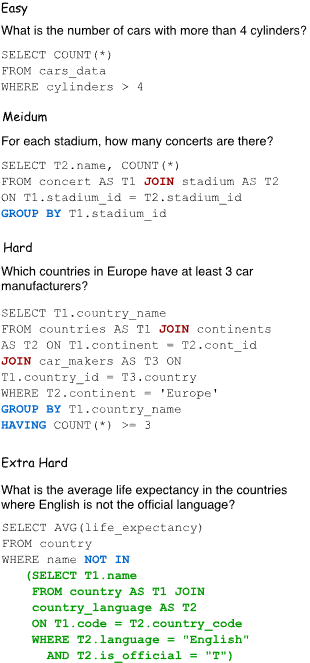
\includegraphics[width=0.35\textwidth]{image.png}
\caption{SQL query examples in 4 hardness levels. Credit: Spider [1]}
\label{fig:hardness-levels}
\end{figure}

\subsection{Prompting and Input}
\label{sec:prompting}

Each model receives three pieces of information in a single zero-shot user turn: a system instruction explaining its role as a Text-to-SQL generator, the database schema (table names, column names, primary keys, and foreign-key relationships, with no example rows), and the natural-language question. No few-shot examples are provided, so that the experiment measures each model's ability to generate SQL from instructions and schema information alone, without the confound of examples steering its output style. The prompt template is identical across all three models, so that differences in performance can be attributed to the models rather than to differences in prompting.

\textbf{Prompt template:}
\begin{verbatim}
Given the following SQLite database schema, write a SQL query that answers
the question.

{schema}

Question: {question}

Respond with only the SQL query in a ```sql code block.
\end{verbatim}

See \hyperref[sec:appendix1]{Appendix 1} for a worked example: a full schema, a question, and the resulting filled prompt.

\subsection{SQL Extraction}
\label{sec:sql-extraction}

For each sample, we decode the model's generated tokens into text using the model-specific tokenizer, and check for the presence of a \texttt{</think>} token. If \texttt{</think>} was generated, we take all text generated before \texttt{</think>} as the reasoning trace and all text to the right as the output SQL; DeepSeek-R1-Distill-Qwen-1.5B is the only model of the three that can emit this token. The SQL is then extracted from the first \texttt{```sql} code block in that remaining text. The extracted SQL is passed to the evaluation script as-is. Outputs that cannot be extracted or parsed are counted as incorrect on every metric rather than excluded from the evaluation, as unusable output is a task failure (see \ref{sec:evaluation-metrics} and \ref{sec:invalid-outputs}).

\subsection{Inference Settings}
\label{sec:inference-settings}

All models are evaluated using the same decoding configuration: greedy decoding (temperature and top-p are not applicable) for consistent, reproducible results between runs. The maximum output length differs by model: 256 tokens for Qwen3-0.6B, and 4096 tokens for both Qwen3-4B and DeepSeek-R1-Distill-Qwen-1.5B. For DeepSeek, the larger budget is needed because its output also has to contain a full reasoning trace rather than only the SQL query; Qwen3-4B is given the same, larger budget as DeepSeek so that a tighter token limit can be ruled out as the reason for any difference between them on invalid-output rate (\ref{sec:invalid-outputs}) or inference time (\ref{sec:efficiency}). Qwen3-0.6B and Qwen3-4B are both run with thinking mode off (both support it). DeepSeek-R1-Distill-Qwen-1.5B always produces a reasoning trace and has no documented way to disable thinking mode, so it is evaluated as the reasoning condition against the two non-reasoning Qwen3 models. All inference runs on the same 1x RTX 4090 GPU described in \ref{sec:models}, with batch size 1.

\subsection{Evaluation}
\label{sec:evaluation-metrics}

We evaluate the output using the same metrics as the Spider paper [1]. These are:

\begin{enumerate}
\item Component Matching
    \begin{itemize}
        \item For each of the following components:
        \begin{itemize}
            \item SELECT
            \item WHERE
            \item GROUP BY
            \item ORDER BY
            \item KEYWORDS (including all SQL keywords without column names and operators)
        \end{itemize}
        \item Decompose each component in the prediction and ground truth as bags of several sub-components and check whether or not these two sets of components match completely.
        \item Checks accuracy, recall, and F1
    \end{itemize}
\item Exact Matching Accuracy
    \begin{itemize}
        \item We measure whether the generated query as a whole is equivalent to the last section
        \item The generated query is correct only if all components are correct
        \item Checks only accuracy
    \end{itemize}
\item Execution Accuracy
    \begin{itemize}
        \item A list of gold values for each question is given
        \item We measure how many gold values the generated query extracts when executed
        \item Checks only accuracy
    \end{itemize}
\end{enumerate}

If output is invalid or unparsable, then it fails all 3 dimensions (component matching, exact matching, execution accuracy), consistent with how \ref{sec:sql-extraction} extracts and passes SQL to this evaluation script. This is reasonable as invalid/unparsable output cannot be applied to SQL and thus must be avoided and penalized heavily; Results~\ref{sec:invalid-outputs} reports how often this happens for each model.

\section{Task 1 -- RQ1: Results}
\label{sec:rq1-results}

\subsection{Overall Model Performance}
\label{sec:overall-performance}

Below we report how Qwen3-0.6B, Qwen3-4B, and Deepseek-R1-Distill-Qwen3-1.5B perform on the Spider benchmark across all 3 metrics (Component Matching, Exact Matching Accuracy, Execution Accuracy). We calculate the values per problem difficulty as well as overall, and display them in the below tables.

\begin{table}[H]
\centering
\footnotesize
\caption{Overall performance summary, aggregated across all difficulties (all 1034 problems). Component matching is accuracy / recall / F1 (macro-averaged, see the note on table~\ref{tab:difficulty-component} in \ref{sec:rq1-interpretation}). Per-difficulty breakdowns are in tables~\ref{tab:difficulty-component}--\ref{tab:difficulty-execution}.}
\label{tab:overall-performance}
\resizebox{\textwidth}{!}{%
\begin{tabular}{lllccc}
\toprule
Model & Parameters & Category & Component matching & Exact matching & Execution accuracy \\
\midrule
Qwen3-0.6B & 0.6B & Decoder-only & 0.628 / 0.209 / 0.314 & 0.099 & 0.209 \\
Qwen3-4B & 4B & Decoder-only & 0.797 / 0.306 / 0.442 & 0.256 & 0.353 \\
DeepSeek-R1-Distill-Qwen-1.5B & 1.5B & Reasoning & 0.661 / 0.174 / 0.275 & 0.085 & 0.121 \\
\bottomrule
\end{tabular}}
\end{table}

All models are evaluated zero-shot with the same prompt on the 20 databases of the Spider dev set. Aggregated across all difficulties and databases, every model is still far from solving the task: execution accuracy ranges from 0.121 (DeepSeek) to 0.353 (Qwen3-4B) and exact matching accuracy from 0.085 (DeepSeek) to 0.256 (Qwen3-4B). Execution accuracy is higher than exact matching accuracy for all three models (for example 0.353 vs.\ 0.256 for Qwen3-4B), which suggests that at least some of the queries that return the correct result are written differently from the gold SQL (see \ref{sec:rq1-interpretation} for more on this relationship). Of the three models, Qwen3-4B is now the best on almost every metric, database, and difficulty level; \ref{sec:by-database} and \ref{sec:rq1-interpretation} quantify how consistently. Table~\ref{tab:inference-time} reports the efficiency side of this comparison: inference time per example.

\subsection{Performance by Query Difficulty}
\label{sec:by-difficulty}

\begin{table}[H]
\centering
\footnotesize
\caption{Component matching (accuracy / recall / F1) by difficulty.}
\label{tab:difficulty-component}
\begin{tabular}{lcc}
\toprule
Model & easy & medium \\
\midrule
Problems (n) & 248 & 446 \\
Qwen3-0.6B & 0.675 / 0.308 / 0.423 & 0.582 / 0.235 / 0.334 \\
Qwen3-4B & 0.838 / 0.574 / 0.681 & 0.670 / 0.306 / 0.420 \\
DeepSeek-R1-Distill-Qwen-1.5B & 0.566 / 0.288 / 0.382 & 0.642 / 0.185 / 0.287 \\
\bottomrule
\end{tabular}

\vspace{0.5em}

\begin{tabular}{lccc}
\toprule
Model & hard & extra & all \\
\midrule
Problems (n) & 174 & 166 & 1034 \\
Qwen3-0.6B & 0.540 / 0.141 / 0.223 & 0.578 / 0.160 / 0.250 & 0.628 / 0.209 / 0.314 \\
Qwen3-4B & 0.796 / 0.262 / 0.394 & 0.485 / 0.150 / 0.229 & 0.797 / 0.306 / 0.442 \\
DeepSeek-R1-Distill-Qwen-1.5B & 0.543 / 0.113 / 0.187 & 0.389 / 0.104 / 0.164 & 0.661 / 0.174 / 0.275 \\
\bottomrule
\end{tabular}
\end{table}

\begin{table}[H]
\centering
\footnotesize
\caption{Exact matching accuracy by difficulty.}
\label{tab:difficulty-exact}
\begin{tabular}{lccccc}
\toprule
Model & easy & medium & hard & extra & all \\
\midrule
Problems (n) & 248 & 446 & 174 & 166 & 1034 \\
Qwen3-0.6B & 0.157 & 0.137 & 0.006 & 0.006 & 0.099 \\
Qwen3-4B & 0.508 & 0.262 & 0.115 & 0.012 & 0.256 \\
DeepSeek-R1-Distill-Qwen-1.5B & 0.214 & 0.078 & 0.000 & 0.000 & 0.085 \\
\bottomrule
\end{tabular}
\end{table}

\begin{table}[H]
\centering
\footnotesize
\caption{Execution accuracy by difficulty.}
\label{tab:difficulty-execution}
\begin{tabular}{lccccc}
\toprule
Model & easy & medium & hard & extra & all \\
\midrule
Problems (n) & 248 & 446 & 174 & 166 & 1034 \\
Qwen3-0.6B & 0.210 & 0.276 & 0.126 & 0.114 & 0.209 \\
Qwen3-4B & 0.565 & 0.345 & 0.276 & 0.139 & 0.353 \\
DeepSeek-R1-Distill-Qwen-1.5B & 0.258 & 0.128 & 0.017 & 0.006 & 0.121 \\
\bottomrule
\end{tabular}
\end{table}

We break every metric down by the Spider Hardness Criteria (\ref{sec:eval-data}) as query difficulty is a first-order driver of Text-to-SQL performance; comparing models only in aggregate would hide whether a model's advantage holds up as queries get harder.

Performance decreases with difficulty for every model, but the decrease is steepest for Qwen3-0.6B and DeepSeek: their exact matching and execution accuracy are both at most 0.034 and 0.126 respectively on hard and extra problems, down from as high as 0.210-0.258 (easy execution) on the easiest problems (table~\ref{tab:difficulty-exact} and table~\ref{tab:difficulty-execution}). Qwen3-4B degrades on the same relative scale but from a much higher starting point, from 0.508 easy exact matching / 0.565 easy execution accuracy down to 0.012 extra exact matching / 0.139 extra execution accuracy. Despite the degredation, it remains the best of the three models at every single difficulty level on both metrics (tables~\ref{tab:difficulty-exact}--\ref{tab:difficulty-execution}).

\subsection{Performance by Database}
\label{sec:by-database}

We also break execution and exact matching accuracy down by each of the 20 Spider dev databases. Qwen3-4B has the highest execution accuracy on 17 of the 20 databases outright (plus a tie on one more) and the highest exact matching accuracy on 18 of 20, while DeepSeek-R1-Distill-Qwen-1.5B is never highest on either metric; Qwen3-0.6B wins outright only on orchestra and battle\_death. Databases with few problems (real\_estate\_properties with n=4, voter\_1 with n=15, battle\_death with n=16, and museum\_visit with n=18) are too small to rank the models reliably, since a single problem changes a score by 6 to 25 percentage points. Execution accuracy ranges from 0.10 (course\_teach) to 0.53 (singer) for Qwen3-0.6B, from 0.19 (battle\_death) to 0.60 (singer) for Qwen3-4B, and from 0.00 (concert\_singer) to 0.27 (singer and voter\_1) for DeepSeek-R1-Distill-Qwen-1.5B (\hyperref[tab:db-execution]{Table 5}). The pattern on exact matching accuracy is just as one-sided (\hyperref[tab:db-exact]{Table 6}): Qwen3-4B is highest on 18 of 20 databases, ties Qwen3-0.6B on orchestra, and loses only on battle\_death; DeepSeek's exact matching accuracy is never the highest of the three, coming closest on flight\_2 (0.200 vs.\ Qwen3-4B's 0.350 and Qwen3-0.6B's 0.075). The full per-database tables and discussion are in \hyperref[sec:appendix2]{Appendix 2}.

\subsection{Invalid and Unparseable Outputs}
\label{sec:invalid-outputs}

We also count how often each model's output cannot be used as SQL at all: it either never produces a usable query within the token budget (\ref{sec:inference-settings}) or is truncated before finishing one. Per \ref{sec:evaluation-metrics}, these count as failures on every metric rather than being excluded, and this is a direct measure of how reliably each model follows the ``respond with only a SQL query'' instruction, independent of whether the SQL it does produce is correct. Qwen3-0.6B's invalid rate is 2.2\%, Qwen3-4B's is 0.0\%, and DeepSeek-R1-Distill-Qwen-1.5B's is 9.7\%, about 4x higher than Qwen3-0.6B's despite having the same 4096-token budget as Qwen3-4B (\ref{sec:inference-settings}), i.e. a larger token budget did not cause Qwen3-4B to run on or produce unusable output the way it does for DeepSeek. \ref{sec:rq1-interpretation} breaks DeepSeek's failures down further by difficulty and by why the generation failed (tables~\ref{tab:deepseek-outcome}--\ref{tab:deepseek-unfinished-by-difficulty}).

\subsection{Efficiency Measures}
\label{sec:efficiency}

\begin{table}[H]
\centering
\footnotesize
\caption{Output tokens per example}
\label{tab:tokens-per-example}
\begin{tabular}{lccccc}
\toprule
Model & easy & medium & hard & extra & all \\
\midrule
Qwen3-0.6B & 27.5 & 44.7 & 53.7 & 69.9 & 46.1 \\
Qwen3-4B & 23.6 & 37.3 & 46.2 & 59.0 & 39.0 \\
DeepSeek-R1-Distill-Qwen-1.5B & 610.8 & 768.4 & 1096.0 & 1176.9 & 851.3 \\
\bottomrule
\end{tabular}
\end{table}

Inference time is measured from the start of generation to the complete batch output, per batch of 1 example, excluding tokenization, model loading, and warm-up.

\begin{table}[H]
\centering
\footnotesize
\caption{Inference time.}
\label{tab:inference-time}
\begin{tabular}{lcc}
\toprule
Model & Total wall time (s) & Avg.\ time per example (s) \\
\midrule
Qwen3-0.6B & 123.9 & 0.120 \\
Qwen3-4B & 109.1 & 0.106 \\
DeepSeek-R1-Distill-Qwen-1.5B & 3059.8 & 2.959 \\
\bottomrule
\end{tabular}
\end{table}

DeepSeek is about 25x slower per example than Qwen3-0.6B and 28x slower than Qwen3-4B, consistent with its much higher average token count (table~\ref{tab:tokens-per-example}). Qwen3-4B, despite having about 7x as many parameters as Qwen3-0.6B, is marginally faster per example (0.106s vs.\ 0.120s), consistent with it generating fewer tokens on average (39.0 vs.\ 46.1, table~\ref{tab:tokens-per-example}) despite having the same 16x larger token budget as DeepSeek (\ref{sec:inference-settings}).

\begin{table}[H]
\centering
\footnotesize
\caption{DeepSeek-R1-Distill-Qwen-1.5B by generation outcome. ``Cut'' means the generation reached the 4096-token limit.}
\label{tab:deepseek-outcome}
\begin{tabular}{lccccc}
\toprule
Outcome & Problems (n) & Share & Avg.\ tokens & Exact match & Component F1 \\
\midrule
Finished with SQL & 934 & 90.3\% & 512 & 0.094 & 0.286 \\
Finished, no usable SQL & 2 & 0.2\% & 284 & 0.000 & 0.100 \\
Cut while answering (after \texttt{</think>}) & 13 & 1.3\% & 4096 & 0.000 & 0.096 \\
Cut while thinking (no \texttt{</think>}) & 85 & 8.2\% & 4096 & 0.000 & 0.093 \\
All & 1034 & 100\% & 851 & 0.085 & 0.275 \\
\bottomrule
\end{tabular}
\end{table}

\begin{table}[H]
\centering
\footnotesize
\caption{The same 934 questions that DeepSeek finished, for all three models.}
\label{tab:deepseek-finished-934}
\begin{tabular}{lcc}
\toprule
Model & Exact match & Component F1 \\
\midrule
DeepSeek-R1-Distill-Qwen-1.5B & 0.094 & 0.286 \\
Qwen3-0.6B & 0.103 & 0.317 \\
Qwen3-4B & 0.257 & 0.440 \\
\bottomrule
\end{tabular}
\end{table}

\begin{table}[H]
\centering
\footnotesize
\caption{Are the cut-off DeepSeek generations infinite self-repetition loops? A text that repeats itself compresses well, so a low compression ratio of the last 3000 characters indicates a loop.}
\label{tab:deepseek-repetition}
\begin{tabular}{lcccc}
\toprule
Generations & n & Median compression ratio & Ratio $<$ 0.15 & Last 150 characters repeat 3 or more times \\
\midrule
Cut off & 98 & 0.095 & 95.9\% & 96.9\% \\
Finished & 936 & 0.418 & 0.0\% & 0.2\% \\
\bottomrule
\end{tabular}
\end{table}

\begin{table}[H]
\centering
\footnotesize
\caption{Share of DeepSeek generations that did not finish with SQL, by difficulty.}
\label{tab:deepseek-unfinished-by-difficulty}
\begin{tabular}{lccccc}
\toprule
 & easy & medium & hard & extra & all \\
\midrule
Problems (n) & 248 & 446 & 174 & 166 & 1034 \\
Not finished with SQL (n) & 15 & 33 & 25 & 27 & 100 \\
Share & 6.0\% & 7.4\% & 14.4\% & 16.3\% & 9.7\% \\
\bottomrule
\end{tabular}
\end{table}

\section{Interpretation and Answer to Research Question (RQ1)}
\label{sec:rq1-interpretation}

\textbf{RQ1:} How do (selected) LLMs perform on cross-domain Text-to-SQL?

\vspace{10px}

All three models are still far from solving the task in this zero-shot setting: exact matching accuracy ranges from 0.085 to 0.256 and execution accuracy from 0.121 to 0.353 (table~\ref{tab:overall-performance}). Difficulty and database effects are discussed in \ref{sec:by-difficulty} and \ref{sec:by-database}; here we interpret the effects of model size and reasoning architecture and the exact-match/execution-accuracy relationship, and state the answer to RQ1 as three findings.

\textbf{First, within the Qwen family, scale is a strong and almost uniform predictor of performance, but an intermediate-size reasoning model from the Deepseek family still loses to the smallest model in the Qwen family.} Aggregated across all difficulties, Qwen3-4B has the best component matching (0.797 / 0.306 / 0.442), exact matching (0.256), and execution accuracy (0.353) of the three (table~\ref{tab:overall-performance}), and it beats Qwen3-0.6B on exact matching and execution accuracy at every individual difficulty level, including hard (0.115 vs.\ 0.006) and extra (0.012 vs.\ 0.006), where the smaller model solves almost nothing (tables~\ref{tab:difficulty-exact}--\ref{tab:difficulty-execution}). This is the largest, most consistent effect in the RQ1 results. The one exception is component matching on extra-hard problems, where Qwen3-0.6B's accuracy, recall, and F1 (0.578 / 0.160 / 0.250) are all slightly higher than Qwen3-4B's (0.485 / 0.150 / 0.229), the only point in the RQ1 results where the smaller Qwen3 model wins outright (table~\ref{tab:difficulty-component}). DeepSeek-R1-Distill-Qwen-1.5B sits between the two Qwen3 models in parameter count (1.5B) and is the only one that reasons, yet it is the lowest of the three on every aggregate metric (0.275 component F1, 0.085 exact matching, 0.121 execution accuracy) except its own component-matching accuracy (0.661 vs.\ 0.628 for Qwen3-0.6B). Thus, scale predicts performance well within a family, but does not transfer across the reasoning/non-reasoning boundary: having more parameters than Qwen3-0.6B did not help DeepSeek catch up to it.

\textbf{Second, the reasoning architecture itself, not parameter count, is the main driver of DeepSeek's low score.} Its invalid-output rate (9.7\%) is markedly higher than Qwen3-0.6B's (2.2\%) and Qwen3-4B's (0.0\% in this run) (\ref{sec:invalid-outputs}). In tables~\ref{tab:deepseek-outcome}--\ref{tab:deepseek-unfinished-by-difficulty}, 100 of 1034 generations (9.7\%) end without usable SQL. 85 never leave the reasoning phase, 13 are cut while writing the answer, and 2 finish without SQL. The number of unusable SQL generations also grows with difficulty, from 6.0\% on easy to 16.3\% on extra problems. These are not cases of long productive reasoning either: 95.9\% of the cut-off generations are highly self-repetitive (compression ratio below 0.15, median compression ratio 0.095, vs.\ 0.418 for finished generations), rewriting the same query and repeating phrases like ``So the final query is:'' without converging. Finishing does not make it better either: on the 934 questions DeepSeek does finish, its exact matching (0.094) and component F1 (0.286) are still below Qwen3-0.6B's on the same questions (0.103 / 0.317) and far below Qwen3-4B's (0.257 / 0.440), despite generating 512 tokens per question on average there, against 46 and 39 tokens overall for Qwen3-0.6B and Qwen3-4B (about 18x and 22x fewer). This extra length also costs time: DeepSeek is 25-28x slower per example than either Qwen3 model (\ref{sec:efficiency}). The reasoning trace mostly lengthens the output and sometimes never terminates, without improving the SQL when it does, and size alone is not the explanation, since Qwen3-4B is both bigger than DeepSeek and the best model in the comparison. Thus, reasoning architecture itself, not the parameter count, is the main driver of DeepSeek's low score.

\textbf{Third, query difficulty has a substantial, consistent effect on every model, including the best one.} Exact matching and execution accuracy both fall sharply from easy to extra-hard problems for all three models (\ref{sec:by-difficulty}). Qwen3-4B's drop is from a much higher base (0.508 to 0.012 exact matching, 0.565 to 0.139 execution accuracy) and it remains the best model at every difficulty level on both metrics, but the drop itself is just as steep in relative terms as for the other two models, and the hardest problems remain largely unsolved even for it.

\textbf{Exact match vs.\ execution accuracy.} For all three models, execution accuracy aggregated across all difficulties exceeds exact matching accuracy (table~\ref{tab:overall-performance}): 0.209 vs.\ 0.099 for Qwen3-0.6B, 0.353 vs.\ 0.256 for Qwen3-4B, and 0.121 vs.\ 0.085 for DeepSeek. Since exact matching requires every SQL component to match the gold query while execution accuracy only requires the same result set, this gap indicates each model writes some queries that are valid and correct but phrased differently from the gold SQL (e.g.\ a different but equivalent join order, or an explicit column list where the gold query uses \texttt{SELECT *}). The gap is widest for Qwen3-0.6B (11.0 points), close behind for Qwen3-4B (9.7 points), and narrowest for DeepSeek (3.6 points); DeepSeek's narrower gap reflects it producing fewer alternative-but-valid queries. Qwen3-4B's gap is almost as wide as Qwen3-0.6B's despite much higher absolute accuracy, so scaling up within the Qwen3 family raises both Exact Match Accuracy and Execution Accuracy together rather than closing the gap between them.

\textbf{Limitations.} Our working hypothesis is that Text-to-SQL at this scale does not benefit from an explicit reasoning trace, and that a non-reasoning model is sufficient, with performance instead scaling with parameter count within a fixed model family. The results are consistent with this hypothesis. However, they do not establish that Text-to-SQL is too simple for reasoning models in general due to several factors:

\begin{itemize}
\item \textbf{Truncation and failed outputs for DeepSeek.} These count as failures on every metric and lower its recall, exact matching, and execution scores, but table~\ref{tab:deepseek-finished-934} shows removing them would not change the ranking (DeepSeek is also lower on the questions it finished), and table~\ref{tab:deepseek-repetition} shows the cut-off generations are repetition loops, so a larger token budget is unlikely to rescue them.
\item \textbf{Model differences beyond reasoning.} Qwen3-0.6B and Qwen3-4B share a model family, isolating the effect of scale between them, but DeepSeek differs from both in family, size, and pretraining/post-training, not only in whether it reasons; it is also a distilled model, so the effect of reasoning cannot be fully separated from distillation quality.
\item \textbf{Aggregated component matching.} The component matching figures in table~\ref{tab:difficulty-component} (and in table~\ref{tab:overall-performance}) are our own macro-average (mean of the 10 per-component accuracy and recall scores, with F1 computed from these two means), not a number reported by Spider.
\end{itemize}

Overall, in this zero-shot, cross-domain setting, a larger non-reasoning decoder-only model (Qwen3-4B, 4B) clearly outperforms both a same-family model at under a sixth its size (Qwen3-0.6B) and a reasoning model of intermediate size from a different family (DeepSeek-R1-Distill-Qwen-1.5B, 1.5B), while also being faster per example than either. None of the three models solve more than half of even the easiest problems or more than a small fraction of hard or extra-hard queries. This answers RQ1 for the three models evaluated.
 into REPORT.tex in place of the current inline
% "Task 1 -- RQ1: Methodology & Results" / "Task 1 -- RQ1: Results" content.
% REPORT.tex already loads every package this fragment needs (booktabs, array,
% graphicx, float, caption, hyperref), so no extra preamble is required.
%
% Annotations made while converting this to reference-based numbering:
%  - All \subsection*{N.M ...} / \section*{...} became real, numbered
%    \section/\subsection commands with the leading "N.M" stripped from the
%    title text (LaTeX now generates it), each with a \label. The former
%    \subsection*{3. Interpretation...} is promoted to a top-level \section,
%    since it was already numbered as a peer of Parts 1 and 2, not a child
%    of Part 2.
%  - Every table/figure got a \label right after its \caption, and every
%    in-text "table 1", "tables 2-4", "2.2", "Appendix 2", etc. became a
%    \ref (or \hyperref for Appendix 2/3, which live outside this file --
%    see note below). Because the Models table (1.1) is now counted and the
%    Appendix 2/3 tables are not part of this file's sequential numbering,
%    the printed table numbers shift versus the pasted draft (e.g. "table 1"
%    -> Table 2, "table 8" -> Table 6); every mention uses \ref, so this is
%    self-consistent and will stay correct if tables move again.
%  - Fixed a leftover inconsistency in 1.5: the draft's 1.1 and 2.5 both
%    state batch size 1 (confirmed correct), but 1.5 still said "batch size
%    128" (leftover from an earlier draft) -- corrected to 1.
%  - Both TODOs in the pasted draft are resolved inline: 2.2 now cites
%    Tables 4-5 directly instead of a placeholder, and 2.3 now cites the
%    concrete per-database numbers from Appendix 2 (pulled from REPORT.tex's
%    existing Appendix 2 prose) instead of a placeholder.
%  - The Overall Performance table's caption promises "the note on table 2
%    in 3" (i.e. a note about macro-averaged component matching, to appear
%    in the Interpretation section), but the pasted draft's Limitations list
%    dropped that bullet (it only kept "Truncation" and "Model differences").
%    Restored the "Aggregated component matching" bullet from the prior
%    REPORT.tex draft so the caption's forward reference resolves to real
%    content; this is a content restoration, not just a labeling change,
%    so flagging it here. The other previously-present bullet ("Single run
%    and sample size") was NOT restored, since nothing in the new draft
%    points to it -- worth confirming with the author whether that drop was
%    intentional.
%  - Appendix 1/2/3 and their tables (5, 6, 7) live in REPORT.tex, outside
%    this file. REPORT.tex's appendix tables keep their existing manual
%    "Table 5/6/7:" caption numbering (renumbering them would require
%    restructuring the whole document's table order, which is out of scope
%    here); \label{tab:db-execution}, \label{tab:db-exact} and
%    \label{tab:invalid-outputs} were added to those tables in REPORT.tex
%    (additive only, no visible change) so this file can link to them.
%    Since their printed numbers are not auto-generated, this file links to
%    them with \hyperref[label]{5}-style calls (a real clickable link, with
%    text matching the manual number already in their caption) rather than
%    \ref (which would print whatever their true document-order table
%    number is, not 5/6/7).

\section{Task 1 -- RQ1: Methodology \& Results}
\label{sec:rq1-methods}

\textbf{RQ1:} How do (selected) LLMs perform on cross-domain Text-to-SQL?

In this report we evaluate the performance of decoder-only language models as well as reasoning LLMs on cross-domain SQL.

\subsection{Models}
\label{sec:models}

We compare two decoder-only LLMs from the same model family at different scales (Qwen3-0.6B and Qwen3-4B) against one reasoning LLM, so that the comparison isolates the effect of scale within a fixed family from the effect of an explicit reasoning trace, as much as a 3-model study can. All three are accessed as local inference over their bf16 Huggingface checkpoints on 1x NVIDIA GeForce RTX 4090 GPU (no API-based models), so that inference parameters are fully under our control (see \ref{sec:inference-settings}). We evaluate using batch sizes of 1.

\begin{table}[H]
\centering
\footnotesize
\caption{Models compared in RQ1.}
\label{tab:models}
\resizebox{\textwidth}{!}{%
\begin{tabular}{llllll}
\toprule
Model & Category & Parameters & Quantization & Access & Thinking mode \\
\midrule
Qwen3-0.6B [2] & Decoder-only & 0.6B & bf16 (none beyond release precision) & Local, Huggingface checkpoint & Disabled \\
Qwen3-4B [2] & Decoder-only & 4B & bf16 (none beyond release precision) & Local, Huggingface checkpoint & Disabled \\
DeepSeek-R1-Distill-Qwen-1.5B [4] & Reasoning & 1.5B & bf16 (none beyond release precision) & Local, Huggingface checkpoint & Always on (no disable option) \\
\bottomrule
\end{tabular}}
\end{table}

All three are dense (non-MoE) models, so no distinction between total and active parameters applies.

\subsection{Evaluation Data}
\label{sec:eval-data}

We use all 1034 examples in the Spider [1] development split, with no subsampling and therefore no sampling seed to report; every example is included, so the per-database counts below and the per-database results tables (\hyperref[tab:db-execution]{5} and \hyperref[tab:db-exact]{6}) enumerate exactly which examples are used. To evaluate cross-domain performance, we additionally report results separately for each of the 20 databases in the Spider dev set: world\_1 (120 problems), car\_1 (92), cre\_Doc\_Template\_Mgt (84), dog\_kennels (82), flight\_2 (80), student\_transcripts\_tracking (78), wta\_1 (62), tvshow (62), network\_1 (56), concert\_singer (45), pets\_1 (42), poker\_player (40), orchestra (40), employee\_hire\_evaluation (38), course\_teach (30), singer (30), museum\_visit (18), battle\_death (16), voter\_1 (15), and real\_estate\_properties (4).

We also use the Spider Hardness Criteria, where queries are assigned difficulties based on the number of SQL components, selections, and conditions, so that queries that contain more SQL keywords are considered harder.

\begin{figure}[H]
\centering
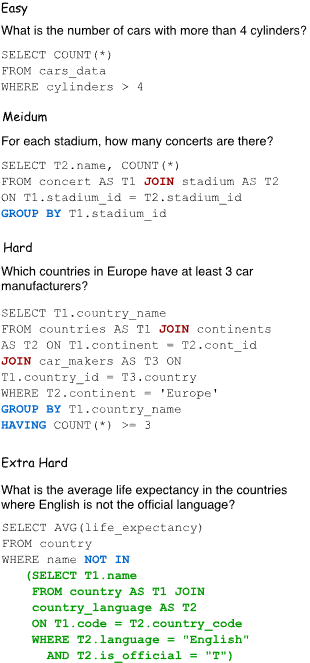
\includegraphics[width=0.35\textwidth]{image.png}
\caption{SQL query examples in 4 hardness levels. Credit: Spider [1]}
\label{fig:hardness-levels}
\end{figure}

\subsection{Prompting and Input}
\label{sec:prompting}

Each model receives three pieces of information in a single zero-shot user turn: a system instruction explaining its role as a Text-to-SQL generator, the database schema (table names, column names, primary keys, and foreign-key relationships, with no example rows), and the natural-language question. No few-shot examples are provided, so that the experiment measures each model's ability to generate SQL from instructions and schema information alone, without the confound of examples steering its output style. The prompt template is identical across all three models, so that differences in performance can be attributed to the models rather than to differences in prompting.

\textbf{Prompt template:}
\begin{verbatim}
Given the following SQLite database schema, write a SQL query that answers
the question.

{schema}

Question: {question}

Respond with only the SQL query in a ```sql code block.
\end{verbatim}

See \hyperref[sec:appendix1]{Appendix 1} for a worked example: a full schema, a question, and the resulting filled prompt.

\subsection{SQL Extraction}
\label{sec:sql-extraction}

For each sample, we decode the model's generated tokens into text using the model-specific tokenizer, and check for the presence of a \texttt{</think>} token. If \texttt{</think>} was generated, we take all text generated before \texttt{</think>} as the reasoning trace and all text to the right as the output SQL; DeepSeek-R1-Distill-Qwen-1.5B is the only model of the three that can emit this token. The SQL is then extracted from the first \texttt{```sql} code block in that remaining text. The extracted SQL is passed to the evaluation script as-is. Outputs that cannot be extracted or parsed are counted as incorrect on every metric rather than excluded from the evaluation, as unusable output is a task failure (see \ref{sec:evaluation-metrics} and \ref{sec:invalid-outputs}).

\subsection{Inference Settings}
\label{sec:inference-settings}

All models are evaluated using the same decoding configuration: greedy decoding (temperature and top-p are not applicable) for consistent, reproducible results between runs. The maximum output length differs by model: 256 tokens for Qwen3-0.6B, and 4096 tokens for both Qwen3-4B and DeepSeek-R1-Distill-Qwen-1.5B. For DeepSeek, the larger budget is needed because its output also has to contain a full reasoning trace rather than only the SQL query; Qwen3-4B is given the same, larger budget as DeepSeek so that a tighter token limit can be ruled out as the reason for any difference between them on invalid-output rate (\ref{sec:invalid-outputs}) or inference time (\ref{sec:efficiency}). Qwen3-0.6B and Qwen3-4B are both run with thinking mode off (both support it). DeepSeek-R1-Distill-Qwen-1.5B always produces a reasoning trace and has no documented way to disable thinking mode, so it is evaluated as the reasoning condition against the two non-reasoning Qwen3 models. All inference runs on the same 1x RTX 4090 GPU described in \ref{sec:models}, with batch size 1.

\subsection{Evaluation}
\label{sec:evaluation-metrics}

We evaluate the output using the same metrics as the Spider paper [1]. These are:

\begin{enumerate}
\item Component Matching
    \begin{itemize}
        \item For each of the following components:
        \begin{itemize}
            \item SELECT
            \item WHERE
            \item GROUP BY
            \item ORDER BY
            \item KEYWORDS (including all SQL keywords without column names and operators)
        \end{itemize}
        \item Decompose each component in the prediction and ground truth as bags of several sub-components and check whether or not these two sets of components match completely.
        \item Checks accuracy, recall, and F1
    \end{itemize}
\item Exact Matching Accuracy
    \begin{itemize}
        \item We measure whether the generated query as a whole is equivalent to the last section
        \item The generated query is correct only if all components are correct
        \item Checks only accuracy
    \end{itemize}
\item Execution Accuracy
    \begin{itemize}
        \item A list of gold values for each question is given
        \item We measure how many gold values the generated query extracts when executed
        \item Checks only accuracy
    \end{itemize}
\end{enumerate}

If output is invalid or unparsable, then it fails all 3 dimensions (component matching, exact matching, execution accuracy), consistent with how \ref{sec:sql-extraction} extracts and passes SQL to this evaluation script. This is reasonable as invalid/unparsable output cannot be applied to SQL and thus must be avoided and penalized heavily; Results~\ref{sec:invalid-outputs} reports how often this happens for each model.

\section{Task 1 -- RQ1: Results}
\label{sec:rq1-results}

\subsection{Overall Model Performance}
\label{sec:overall-performance}

Below we report how Qwen3-0.6B, Qwen3-4B, and Deepseek-R1-Distill-Qwen3-1.5B perform on the Spider benchmark across all 3 metrics (Component Matching, Exact Matching Accuracy, Execution Accuracy). We calculate the values per problem difficulty as well as overall, and display them in the below tables.

\begin{table}[H]
\centering
\footnotesize
\caption{Overall performance summary, aggregated across all difficulties (all 1034 problems). Component matching is accuracy / recall / F1 (macro-averaged, see the note on table~\ref{tab:difficulty-component} in \ref{sec:rq1-interpretation}). Per-difficulty breakdowns are in tables~\ref{tab:difficulty-component}--\ref{tab:difficulty-execution}.}
\label{tab:overall-performance}
\resizebox{\textwidth}{!}{%
\begin{tabular}{lllccc}
\toprule
Model & Parameters & Category & Component matching & Exact matching & Execution accuracy \\
\midrule
Qwen3-0.6B & 0.6B & Decoder-only & 0.628 / 0.209 / 0.314 & 0.099 & 0.209 \\
Qwen3-4B & 4B & Decoder-only & 0.797 / 0.306 / 0.442 & 0.256 & 0.353 \\
DeepSeek-R1-Distill-Qwen-1.5B & 1.5B & Reasoning & 0.661 / 0.174 / 0.275 & 0.085 & 0.121 \\
\bottomrule
\end{tabular}}
\end{table}

All models are evaluated zero-shot with the same prompt on the 20 databases of the Spider dev set. Aggregated across all difficulties and databases, every model is still far from solving the task: execution accuracy ranges from 0.121 (DeepSeek) to 0.353 (Qwen3-4B) and exact matching accuracy from 0.085 (DeepSeek) to 0.256 (Qwen3-4B). Execution accuracy is higher than exact matching accuracy for all three models (for example 0.353 vs.\ 0.256 for Qwen3-4B), which suggests that at least some of the queries that return the correct result are written differently from the gold SQL (see \ref{sec:rq1-interpretation} for more on this relationship). Of the three models, Qwen3-4B is now the best on almost every metric, database, and difficulty level; \ref{sec:by-database} and \ref{sec:rq1-interpretation} quantify how consistently. Table~\ref{tab:inference-time} reports the efficiency side of this comparison: inference time per example.

\subsection{Performance by Query Difficulty}
\label{sec:by-difficulty}

\begin{table}[H]
\centering
\footnotesize
\caption{Component matching (accuracy / recall / F1) by difficulty.}
\label{tab:difficulty-component}
\begin{tabular}{lcc}
\toprule
Model & easy & medium \\
\midrule
Problems (n) & 248 & 446 \\
Qwen3-0.6B & 0.675 / 0.308 / 0.423 & 0.582 / 0.235 / 0.334 \\
Qwen3-4B & 0.838 / 0.574 / 0.681 & 0.670 / 0.306 / 0.420 \\
DeepSeek-R1-Distill-Qwen-1.5B & 0.566 / 0.288 / 0.382 & 0.642 / 0.185 / 0.287 \\
\bottomrule
\end{tabular}

\vspace{0.5em}

\begin{tabular}{lccc}
\toprule
Model & hard & extra & all \\
\midrule
Problems (n) & 174 & 166 & 1034 \\
Qwen3-0.6B & 0.540 / 0.141 / 0.223 & 0.578 / 0.160 / 0.250 & 0.628 / 0.209 / 0.314 \\
Qwen3-4B & 0.796 / 0.262 / 0.394 & 0.485 / 0.150 / 0.229 & 0.797 / 0.306 / 0.442 \\
DeepSeek-R1-Distill-Qwen-1.5B & 0.543 / 0.113 / 0.187 & 0.389 / 0.104 / 0.164 & 0.661 / 0.174 / 0.275 \\
\bottomrule
\end{tabular}
\end{table}

\begin{table}[H]
\centering
\footnotesize
\caption{Exact matching accuracy by difficulty.}
\label{tab:difficulty-exact}
\begin{tabular}{lccccc}
\toprule
Model & easy & medium & hard & extra & all \\
\midrule
Problems (n) & 248 & 446 & 174 & 166 & 1034 \\
Qwen3-0.6B & 0.157 & 0.137 & 0.006 & 0.006 & 0.099 \\
Qwen3-4B & 0.508 & 0.262 & 0.115 & 0.012 & 0.256 \\
DeepSeek-R1-Distill-Qwen-1.5B & 0.214 & 0.078 & 0.000 & 0.000 & 0.085 \\
\bottomrule
\end{tabular}
\end{table}

\begin{table}[H]
\centering
\footnotesize
\caption{Execution accuracy by difficulty.}
\label{tab:difficulty-execution}
\begin{tabular}{lccccc}
\toprule
Model & easy & medium & hard & extra & all \\
\midrule
Problems (n) & 248 & 446 & 174 & 166 & 1034 \\
Qwen3-0.6B & 0.210 & 0.276 & 0.126 & 0.114 & 0.209 \\
Qwen3-4B & 0.565 & 0.345 & 0.276 & 0.139 & 0.353 \\
DeepSeek-R1-Distill-Qwen-1.5B & 0.258 & 0.128 & 0.017 & 0.006 & 0.121 \\
\bottomrule
\end{tabular}
\end{table}

We break every metric down by the Spider Hardness Criteria (\ref{sec:eval-data}) as query difficulty is a first-order driver of Text-to-SQL performance; comparing models only in aggregate would hide whether a model's advantage holds up as queries get harder.

Performance decreases with difficulty for every model, but the decrease is steepest for Qwen3-0.6B and DeepSeek: their exact matching and execution accuracy are both at most 0.034 and 0.126 respectively on hard and extra problems, down from as high as 0.210-0.258 (easy execution) on the easiest problems (table~\ref{tab:difficulty-exact} and table~\ref{tab:difficulty-execution}). Qwen3-4B degrades on the same relative scale but from a much higher starting point, from 0.508 easy exact matching / 0.565 easy execution accuracy down to 0.012 extra exact matching / 0.139 extra execution accuracy. Despite the degredation, it remains the best of the three models at every single difficulty level on both metrics (tables~\ref{tab:difficulty-exact}--\ref{tab:difficulty-execution}).

\subsection{Performance by Database}
\label{sec:by-database}

We also break execution and exact matching accuracy down by each of the 20 Spider dev databases. Qwen3-4B has the highest execution accuracy on 17 of the 20 databases outright (plus a tie on one more) and the highest exact matching accuracy on 18 of 20, while DeepSeek-R1-Distill-Qwen-1.5B is never highest on either metric; Qwen3-0.6B wins outright only on orchestra and battle\_death. Databases with few problems (real\_estate\_properties with n=4, voter\_1 with n=15, battle\_death with n=16, and museum\_visit with n=18) are too small to rank the models reliably, since a single problem changes a score by 6 to 25 percentage points. Execution accuracy ranges from 0.10 (course\_teach) to 0.53 (singer) for Qwen3-0.6B, from 0.19 (battle\_death) to 0.60 (singer) for Qwen3-4B, and from 0.00 (concert\_singer) to 0.27 (singer and voter\_1) for DeepSeek-R1-Distill-Qwen-1.5B (\hyperref[tab:db-execution]{Table 5}). The pattern on exact matching accuracy is just as one-sided (\hyperref[tab:db-exact]{Table 6}): Qwen3-4B is highest on 18 of 20 databases, ties Qwen3-0.6B on orchestra, and loses only on battle\_death; DeepSeek's exact matching accuracy is never the highest of the three, coming closest on flight\_2 (0.200 vs.\ Qwen3-4B's 0.350 and Qwen3-0.6B's 0.075). The full per-database tables and discussion are in \hyperref[sec:appendix2]{Appendix 2}.

\subsection{Invalid and Unparseable Outputs}
\label{sec:invalid-outputs}

We also count how often each model's output cannot be used as SQL at all: it either never produces a usable query within the token budget (\ref{sec:inference-settings}) or is truncated before finishing one. Per \ref{sec:evaluation-metrics}, these count as failures on every metric rather than being excluded, and this is a direct measure of how reliably each model follows the ``respond with only a SQL query'' instruction, independent of whether the SQL it does produce is correct. Qwen3-0.6B's invalid rate is 2.2\%, Qwen3-4B's is 0.0\%, and DeepSeek-R1-Distill-Qwen-1.5B's is 9.7\%, about 4x higher than Qwen3-0.6B's despite having the same 4096-token budget as Qwen3-4B (\ref{sec:inference-settings}), i.e. a larger token budget did not cause Qwen3-4B to run on or produce unusable output the way it does for DeepSeek. \ref{sec:rq1-interpretation} breaks DeepSeek's failures down further by difficulty and by why the generation failed (tables~\ref{tab:deepseek-outcome}--\ref{tab:deepseek-unfinished-by-difficulty}).

\subsection{Efficiency Measures}
\label{sec:efficiency}

\begin{table}[H]
\centering
\footnotesize
\caption{Output tokens per example}
\label{tab:tokens-per-example}
\begin{tabular}{lccccc}
\toprule
Model & easy & medium & hard & extra & all \\
\midrule
Qwen3-0.6B & 27.5 & 44.7 & 53.7 & 69.9 & 46.1 \\
Qwen3-4B & 23.6 & 37.3 & 46.2 & 59.0 & 39.0 \\
DeepSeek-R1-Distill-Qwen-1.5B & 610.8 & 768.4 & 1096.0 & 1176.9 & 851.3 \\
\bottomrule
\end{tabular}
\end{table}

Inference time is measured from the start of generation to the complete batch output, per batch of 1 example, excluding tokenization, model loading, and warm-up.

\begin{table}[H]
\centering
\footnotesize
\caption{Inference time.}
\label{tab:inference-time}
\begin{tabular}{lcc}
\toprule
Model & Total wall time (s) & Avg.\ time per example (s) \\
\midrule
Qwen3-0.6B & 123.9 & 0.120 \\
Qwen3-4B & 109.1 & 0.106 \\
DeepSeek-R1-Distill-Qwen-1.5B & 3059.8 & 2.959 \\
\bottomrule
\end{tabular}
\end{table}

DeepSeek is about 25x slower per example than Qwen3-0.6B and 28x slower than Qwen3-4B, consistent with its much higher average token count (table~\ref{tab:tokens-per-example}). Qwen3-4B, despite having about 7x as many parameters as Qwen3-0.6B, is marginally faster per example (0.106s vs.\ 0.120s), consistent with it generating fewer tokens on average (39.0 vs.\ 46.1, table~\ref{tab:tokens-per-example}) despite having the same 16x larger token budget as DeepSeek (\ref{sec:inference-settings}).

\begin{table}[H]
\centering
\footnotesize
\caption{DeepSeek-R1-Distill-Qwen-1.5B by generation outcome. ``Cut'' means the generation reached the 4096-token limit.}
\label{tab:deepseek-outcome}
\begin{tabular}{lccccc}
\toprule
Outcome & Problems (n) & Share & Avg.\ tokens & Exact match & Component F1 \\
\midrule
Finished with SQL & 934 & 90.3\% & 512 & 0.094 & 0.286 \\
Finished, no usable SQL & 2 & 0.2\% & 284 & 0.000 & 0.100 \\
Cut while answering (after \texttt{</think>}) & 13 & 1.3\% & 4096 & 0.000 & 0.096 \\
Cut while thinking (no \texttt{</think>}) & 85 & 8.2\% & 4096 & 0.000 & 0.093 \\
All & 1034 & 100\% & 851 & 0.085 & 0.275 \\
\bottomrule
\end{tabular}
\end{table}

\begin{table}[H]
\centering
\footnotesize
\caption{The same 934 questions that DeepSeek finished, for all three models.}
\label{tab:deepseek-finished-934}
\begin{tabular}{lcc}
\toprule
Model & Exact match & Component F1 \\
\midrule
DeepSeek-R1-Distill-Qwen-1.5B & 0.094 & 0.286 \\
Qwen3-0.6B & 0.103 & 0.317 \\
Qwen3-4B & 0.257 & 0.440 \\
\bottomrule
\end{tabular}
\end{table}

\begin{table}[H]
\centering
\footnotesize
\caption{Are the cut-off DeepSeek generations infinite self-repetition loops? A text that repeats itself compresses well, so a low compression ratio of the last 3000 characters indicates a loop.}
\label{tab:deepseek-repetition}
\begin{tabular}{lcccc}
\toprule
Generations & n & Median compression ratio & Ratio $<$ 0.15 & Last 150 characters repeat 3 or more times \\
\midrule
Cut off & 98 & 0.095 & 95.9\% & 96.9\% \\
Finished & 936 & 0.418 & 0.0\% & 0.2\% \\
\bottomrule
\end{tabular}
\end{table}

\begin{table}[H]
\centering
\footnotesize
\caption{Share of DeepSeek generations that did not finish with SQL, by difficulty.}
\label{tab:deepseek-unfinished-by-difficulty}
\begin{tabular}{lccccc}
\toprule
 & easy & medium & hard & extra & all \\
\midrule
Problems (n) & 248 & 446 & 174 & 166 & 1034 \\
Not finished with SQL (n) & 15 & 33 & 25 & 27 & 100 \\
Share & 6.0\% & 7.4\% & 14.4\% & 16.3\% & 9.7\% \\
\bottomrule
\end{tabular}
\end{table}

\section{Interpretation and Answer to Research Question (RQ1)}
\label{sec:rq1-interpretation}

\textbf{RQ1:} How do (selected) LLMs perform on cross-domain Text-to-SQL?

\vspace{10px}

All three models are still far from solving the task in this zero-shot setting: exact matching accuracy ranges from 0.085 to 0.256 and execution accuracy from 0.121 to 0.353 (table~\ref{tab:overall-performance}). Difficulty and database effects are discussed in \ref{sec:by-difficulty} and \ref{sec:by-database}; here we interpret the effects of model size and reasoning architecture and the exact-match/execution-accuracy relationship, and state the answer to RQ1 as three findings.

\textbf{First, within the Qwen family, scale is a strong and almost uniform predictor of performance, but an intermediate-size reasoning model from the Deepseek family still loses to the smallest model in the Qwen family.} Aggregated across all difficulties, Qwen3-4B has the best component matching (0.797 / 0.306 / 0.442), exact matching (0.256), and execution accuracy (0.353) of the three (table~\ref{tab:overall-performance}), and it beats Qwen3-0.6B on exact matching and execution accuracy at every individual difficulty level, including hard (0.115 vs.\ 0.006) and extra (0.012 vs.\ 0.006), where the smaller model solves almost nothing (tables~\ref{tab:difficulty-exact}--\ref{tab:difficulty-execution}). This is the largest, most consistent effect in the RQ1 results. The one exception is component matching on extra-hard problems, where Qwen3-0.6B's accuracy, recall, and F1 (0.578 / 0.160 / 0.250) are all slightly higher than Qwen3-4B's (0.485 / 0.150 / 0.229), the only point in the RQ1 results where the smaller Qwen3 model wins outright (table~\ref{tab:difficulty-component}). DeepSeek-R1-Distill-Qwen-1.5B sits between the two Qwen3 models in parameter count (1.5B) and is the only one that reasons, yet it is the lowest of the three on every aggregate metric (0.275 component F1, 0.085 exact matching, 0.121 execution accuracy) except its own component-matching accuracy (0.661 vs.\ 0.628 for Qwen3-0.6B). Thus, scale predicts performance well within a family, but does not transfer across the reasoning/non-reasoning boundary: having more parameters than Qwen3-0.6B did not help DeepSeek catch up to it.

\textbf{Second, the reasoning architecture itself, not parameter count, is the main driver of DeepSeek's low score.} Its invalid-output rate (9.7\%) is markedly higher than Qwen3-0.6B's (2.2\%) and Qwen3-4B's (0.0\% in this run) (\ref{sec:invalid-outputs}). In tables~\ref{tab:deepseek-outcome}--\ref{tab:deepseek-unfinished-by-difficulty}, 100 of 1034 generations (9.7\%) end without usable SQL. 85 never leave the reasoning phase, 13 are cut while writing the answer, and 2 finish without SQL. The number of unusable SQL generations also grows with difficulty, from 6.0\% on easy to 16.3\% on extra problems. These are not cases of long productive reasoning either: 95.9\% of the cut-off generations are highly self-repetitive (compression ratio below 0.15, median compression ratio 0.095, vs.\ 0.418 for finished generations), rewriting the same query and repeating phrases like ``So the final query is:'' without converging. Finishing does not make it better either: on the 934 questions DeepSeek does finish, its exact matching (0.094) and component F1 (0.286) are still below Qwen3-0.6B's on the same questions (0.103 / 0.317) and far below Qwen3-4B's (0.257 / 0.440), despite generating 512 tokens per question on average there, against 46 and 39 tokens overall for Qwen3-0.6B and Qwen3-4B (about 18x and 22x fewer). This extra length also costs time: DeepSeek is 25-28x slower per example than either Qwen3 model (\ref{sec:efficiency}). The reasoning trace mostly lengthens the output and sometimes never terminates, without improving the SQL when it does, and size alone is not the explanation, since Qwen3-4B is both bigger than DeepSeek and the best model in the comparison. Thus, reasoning architecture itself, not the parameter count, is the main driver of DeepSeek's low score.

\textbf{Third, query difficulty has a substantial, consistent effect on every model, including the best one.} Exact matching and execution accuracy both fall sharply from easy to extra-hard problems for all three models (\ref{sec:by-difficulty}). Qwen3-4B's drop is from a much higher base (0.508 to 0.012 exact matching, 0.565 to 0.139 execution accuracy) and it remains the best model at every difficulty level on both metrics, but the drop itself is just as steep in relative terms as for the other two models, and the hardest problems remain largely unsolved even for it.

\textbf{Exact match vs.\ execution accuracy.} For all three models, execution accuracy aggregated across all difficulties exceeds exact matching accuracy (table~\ref{tab:overall-performance}): 0.209 vs.\ 0.099 for Qwen3-0.6B, 0.353 vs.\ 0.256 for Qwen3-4B, and 0.121 vs.\ 0.085 for DeepSeek. Since exact matching requires every SQL component to match the gold query while execution accuracy only requires the same result set, this gap indicates each model writes some queries that are valid and correct but phrased differently from the gold SQL (e.g.\ a different but equivalent join order, or an explicit column list where the gold query uses \texttt{SELECT *}). The gap is widest for Qwen3-0.6B (11.0 points), close behind for Qwen3-4B (9.7 points), and narrowest for DeepSeek (3.6 points); DeepSeek's narrower gap reflects it producing fewer alternative-but-valid queries. Qwen3-4B's gap is almost as wide as Qwen3-0.6B's despite much higher absolute accuracy, so scaling up within the Qwen3 family raises both Exact Match Accuracy and Execution Accuracy together rather than closing the gap between them.

\textbf{Limitations.} Our working hypothesis is that Text-to-SQL at this scale does not benefit from an explicit reasoning trace, and that a non-reasoning model is sufficient, with performance instead scaling with parameter count within a fixed model family. The results are consistent with this hypothesis. However, they do not establish that Text-to-SQL is too simple for reasoning models in general due to several factors:

\begin{itemize}
\item \textbf{Truncation and failed outputs for DeepSeek.} These count as failures on every metric and lower its recall, exact matching, and execution scores, but table~\ref{tab:deepseek-finished-934} shows removing them would not change the ranking (DeepSeek is also lower on the questions it finished), and table~\ref{tab:deepseek-repetition} shows the cut-off generations are repetition loops, so a larger token budget is unlikely to rescue them.
\item \textbf{Model differences beyond reasoning.} Qwen3-0.6B and Qwen3-4B share a model family, isolating the effect of scale between them, but DeepSeek differs from both in family, size, and pretraining/post-training, not only in whether it reasons; it is also a distilled model, so the effect of reasoning cannot be fully separated from distillation quality.
\item \textbf{Aggregated component matching.} The component matching figures in table~\ref{tab:difficulty-component} (and in table~\ref{tab:overall-performance}) are our own macro-average (mean of the 10 per-component accuracy and recall scores, with F1 computed from these two means), not a number reported by Spider.
\end{itemize}

Overall, in this zero-shot, cross-domain setting, a larger non-reasoning decoder-only model (Qwen3-4B, 4B) clearly outperforms both a same-family model at under a sixth its size (Qwen3-0.6B) and a reasoning model of intermediate size from a different family (DeepSeek-R1-Distill-Qwen-1.5B, 1.5B), while also being faster per example than either. None of the three models solve more than half of even the easiest problems or more than a small fraction of hard or extra-hard queries. This answers RQ1 for the three models evaluated.
 into REPORT.tex in place of the current inline
% "Task 1 -- RQ1: Methodology & Results" / "Task 1 -- RQ1: Results" content.
% REPORT.tex already loads every package this fragment needs (booktabs, array,
% graphicx, float, caption, hyperref), so no extra preamble is required.
%
% Annotations made while converting this to reference-based numbering:
%  - All \subsection*{N.M ...} / \section*{...} became real, numbered
%    \section/\subsection commands with the leading "N.M" stripped from the
%    title text (LaTeX now generates it), each with a \label. The former
%    \subsection*{3. Interpretation...} is promoted to a top-level \section,
%    since it was already numbered as a peer of Parts 1 and 2, not a child
%    of Part 2.
%  - Every table/figure got a \label right after its \caption, and every
%    in-text "table 1", "tables 2-4", "2.2", "Appendix 2", etc. became a
%    \ref (or \hyperref for Appendix 2/3, which live outside this file --
%    see note below). Because the Models table (1.1) is now counted and the
%    Appendix 2/3 tables are not part of this file's sequential numbering,
%    the printed table numbers shift versus the pasted draft (e.g. "table 1"
%    -> Table 2, "table 8" -> Table 6); every mention uses \ref, so this is
%    self-consistent and will stay correct if tables move again.
%  - Fixed a leftover inconsistency in 1.5: the draft's 1.1 and 2.5 both
%    state batch size 1 (confirmed correct), but 1.5 still said "batch size
%    128" (leftover from an earlier draft) -- corrected to 1.
%  - Both TODOs in the pasted draft are resolved inline: 2.2 now cites
%    Tables 4-5 directly instead of a placeholder, and 2.3 now cites the
%    concrete per-database numbers from Appendix 2 (pulled from REPORT.tex's
%    existing Appendix 2 prose) instead of a placeholder.
%  - The Overall Performance table's caption promises "the note on table 2
%    in 3" (i.e. a note about macro-averaged component matching, to appear
%    in the Interpretation section), but the pasted draft's Limitations list
%    dropped that bullet (it only kept "Truncation" and "Model differences").
%    Restored the "Aggregated component matching" bullet from the prior
%    REPORT.tex draft so the caption's forward reference resolves to real
%    content; this is a content restoration, not just a labeling change,
%    so flagging it here. The other previously-present bullet ("Single run
%    and sample size") was NOT restored, since nothing in the new draft
%    points to it -- worth confirming with the author whether that drop was
%    intentional.
%  - Appendix 1/2/3 and their tables (5, 6, 7) live in REPORT.tex, outside
%    this file. REPORT.tex's appendix tables keep their existing manual
%    "Table 5/6/7:" caption numbering (renumbering them would require
%    restructuring the whole document's table order, which is out of scope
%    here); \label{tab:db-execution}, \label{tab:db-exact} and
%    \label{tab:invalid-outputs} were added to those tables in REPORT.tex
%    (additive only, no visible change) so this file can link to them.
%    Since their printed numbers are not auto-generated, this file links to
%    them with \hyperref[label]{5}-style calls (a real clickable link, with
%    text matching the manual number already in their caption) rather than
%    \ref (which would print whatever their true document-order table
%    number is, not 5/6/7).

\section{Task 1 -- RQ1: Methodology \& Results}
\label{sec:rq1-methods}

\textbf{RQ1:} How do (selected) LLMs perform on cross-domain Text-to-SQL?

In this report we evaluate the performance of decoder-only language models as well as reasoning LLMs on cross-domain SQL.

\subsection{Models}
\label{sec:models}

We compare two decoder-only LLMs from the same model family at different scales (Qwen3-0.6B and Qwen3-4B) against one reasoning LLM, so that the comparison isolates the effect of scale within a fixed family from the effect of an explicit reasoning trace, as much as a 3-model study can. All three are accessed as local inference over their bf16 Huggingface checkpoints on 1x NVIDIA GeForce RTX 4090 GPU (no API-based models), so that inference parameters are fully under our control (see \ref{sec:inference-settings}). We evaluate using batch sizes of 1.

\begin{table}[H]
\centering
\footnotesize
\caption{Models compared in RQ1.}
\label{tab:models}
\resizebox{\textwidth}{!}{%
\begin{tabular}{llllll}
\toprule
Model & Category & Parameters & Quantization & Access & Thinking mode \\
\midrule
Qwen3-0.6B [2] & Decoder-only & 0.6B & bf16 (none beyond release precision) & Local, Huggingface checkpoint & Disabled \\
Qwen3-4B [2] & Decoder-only & 4B & bf16 (none beyond release precision) & Local, Huggingface checkpoint & Disabled \\
DeepSeek-R1-Distill-Qwen-1.5B [4] & Reasoning & 1.5B & bf16 (none beyond release precision) & Local, Huggingface checkpoint & Always on (no disable option) \\
\bottomrule
\end{tabular}}
\end{table}

All three are dense (non-MoE) models, so no distinction between total and active parameters applies.

\subsection{Evaluation Data}
\label{sec:eval-data}

We use all 1034 examples in the Spider [1] development split, with no subsampling and therefore no sampling seed to report; every example is included, so the per-database counts below and the per-database results tables (\hyperref[tab:db-execution]{5} and \hyperref[tab:db-exact]{6}) enumerate exactly which examples are used. To evaluate cross-domain performance, we additionally report results separately for each of the 20 databases in the Spider dev set: world\_1 (120 problems), car\_1 (92), cre\_Doc\_Template\_Mgt (84), dog\_kennels (82), flight\_2 (80), student\_transcripts\_tracking (78), wta\_1 (62), tvshow (62), network\_1 (56), concert\_singer (45), pets\_1 (42), poker\_player (40), orchestra (40), employee\_hire\_evaluation (38), course\_teach (30), singer (30), museum\_visit (18), battle\_death (16), voter\_1 (15), and real\_estate\_properties (4).

We also use the Spider Hardness Criteria, where queries are assigned difficulties based on the number of SQL components, selections, and conditions, so that queries that contain more SQL keywords are considered harder.

\begin{figure}[H]
\centering
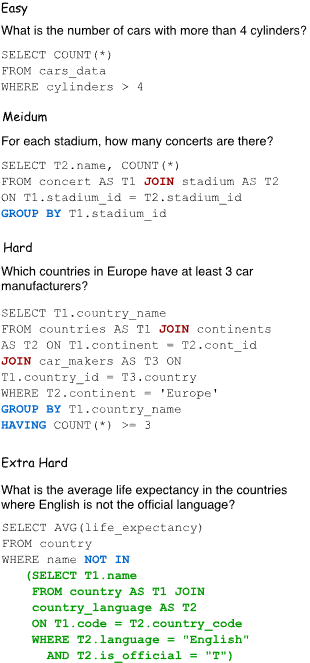
\includegraphics[width=0.35\textwidth]{image.png}
\caption{SQL query examples in 4 hardness levels. Credit: Spider [1]}
\label{fig:hardness-levels}
\end{figure}

\subsection{Prompting and Input}
\label{sec:prompting}

Each model receives three pieces of information in a single zero-shot user turn: a system instruction explaining its role as a Text-to-SQL generator, the database schema (table names, column names, primary keys, and foreign-key relationships, with no example rows), and the natural-language question. No few-shot examples are provided, so that the experiment measures each model's ability to generate SQL from instructions and schema information alone, without the confound of examples steering its output style. The prompt template is identical across all three models, so that differences in performance can be attributed to the models rather than to differences in prompting.

\textbf{Prompt template:}
\begin{verbatim}
Given the following SQLite database schema, write a SQL query that answers
the question.

{schema}

Question: {question}

Respond with only the SQL query in a ```sql code block.
\end{verbatim}

See \hyperref[sec:appendix1]{Appendix 1} for a worked example: a full schema, a question, and the resulting filled prompt.

\subsection{SQL Extraction}
\label{sec:sql-extraction}

For each sample, we decode the model's generated tokens into text using the model-specific tokenizer, and check for the presence of a \texttt{</think>} token. If \texttt{</think>} was generated, we take all text generated before \texttt{</think>} as the reasoning trace and all text to the right as the output SQL; DeepSeek-R1-Distill-Qwen-1.5B is the only model of the three that can emit this token. The SQL is then extracted from the first \texttt{```sql} code block in that remaining text. The extracted SQL is passed to the evaluation script as-is. Outputs that cannot be extracted or parsed are counted as incorrect on every metric rather than excluded from the evaluation, as unusable output is a task failure (see \ref{sec:evaluation-metrics} and \ref{sec:invalid-outputs}).

\subsection{Inference Settings}
\label{sec:inference-settings}

All models are evaluated using the same decoding configuration: greedy decoding (temperature and top-p are not applicable) for consistent, reproducible results between runs. The maximum output length differs by model: 256 tokens for Qwen3-0.6B, and 4096 tokens for both Qwen3-4B and DeepSeek-R1-Distill-Qwen-1.5B. For DeepSeek, the larger budget is needed because its output also has to contain a full reasoning trace rather than only the SQL query; Qwen3-4B is given the same, larger budget as DeepSeek so that a tighter token limit can be ruled out as the reason for any difference between them on invalid-output rate (\ref{sec:invalid-outputs}) or inference time (\ref{sec:efficiency}). Qwen3-0.6B and Qwen3-4B are both run with thinking mode off (both support it). DeepSeek-R1-Distill-Qwen-1.5B always produces a reasoning trace and has no documented way to disable thinking mode, so it is evaluated as the reasoning condition against the two non-reasoning Qwen3 models. All inference runs on the same 1x RTX 4090 GPU described in \ref{sec:models}, with batch size 1.

\subsection{Evaluation}
\label{sec:evaluation-metrics}

We evaluate the output using the same metrics as the Spider paper [1]. These are:

\begin{enumerate}
\item Component Matching
    \begin{itemize}
        \item For each of the following components:
        \begin{itemize}
            \item SELECT
            \item WHERE
            \item GROUP BY
            \item ORDER BY
            \item KEYWORDS (including all SQL keywords without column names and operators)
        \end{itemize}
        \item Decompose each component in the prediction and ground truth as bags of several sub-components and check whether or not these two sets of components match completely.
        \item Checks accuracy, recall, and F1
    \end{itemize}
\item Exact Matching Accuracy
    \begin{itemize}
        \item We measure whether the generated query as a whole is equivalent to the last section
        \item The generated query is correct only if all components are correct
        \item Checks only accuracy
    \end{itemize}
\item Execution Accuracy
    \begin{itemize}
        \item A list of gold values for each question is given
        \item We measure how many gold values the generated query extracts when executed
        \item Checks only accuracy
    \end{itemize}
\end{enumerate}

If output is invalid or unparsable, then it fails all 3 dimensions (component matching, exact matching, execution accuracy), consistent with how \ref{sec:sql-extraction} extracts and passes SQL to this evaluation script. This is reasonable as invalid/unparsable output cannot be applied to SQL and thus must be avoided and penalized heavily; Results~\ref{sec:invalid-outputs} reports how often this happens for each model.

\section{Task 1 -- RQ1: Results}
\label{sec:rq1-results}

\subsection{Overall Model Performance}
\label{sec:overall-performance}

Below we report how Qwen3-0.6B, Qwen3-4B, and Deepseek-R1-Distill-Qwen3-1.5B perform on the Spider benchmark across all 3 metrics (Component Matching, Exact Matching Accuracy, Execution Accuracy). We calculate the values per problem difficulty as well as overall, and display them in the below tables.

\begin{table}[H]
\centering
\footnotesize
\caption{Overall performance summary, aggregated across all difficulties (all 1034 problems). Component matching is accuracy / recall / F1 (macro-averaged, see the note on table~\ref{tab:difficulty-component} in \ref{sec:rq1-interpretation}). Per-difficulty breakdowns are in tables~\ref{tab:difficulty-component}--\ref{tab:difficulty-execution}.}
\label{tab:overall-performance}
\resizebox{\textwidth}{!}{%
\begin{tabular}{lllccc}
\toprule
Model & Parameters & Category & Component matching & Exact matching & Execution accuracy \\
\midrule
Qwen3-0.6B & 0.6B & Decoder-only & 0.628 / 0.209 / 0.314 & 0.099 & 0.209 \\
Qwen3-4B & 4B & Decoder-only & 0.797 / 0.306 / 0.442 & 0.256 & 0.353 \\
DeepSeek-R1-Distill-Qwen-1.5B & 1.5B & Reasoning & 0.661 / 0.174 / 0.275 & 0.085 & 0.121 \\
\bottomrule
\end{tabular}}
\end{table}

All models are evaluated zero-shot with the same prompt on the 20 databases of the Spider dev set. Aggregated across all difficulties and databases, every model is still far from solving the task: execution accuracy ranges from 0.121 (DeepSeek) to 0.353 (Qwen3-4B) and exact matching accuracy from 0.085 (DeepSeek) to 0.256 (Qwen3-4B). Execution accuracy is higher than exact matching accuracy for all three models (for example 0.353 vs.\ 0.256 for Qwen3-4B), which suggests that at least some of the queries that return the correct result are written differently from the gold SQL (see \ref{sec:rq1-interpretation} for more on this relationship). Of the three models, Qwen3-4B is now the best on almost every metric, database, and difficulty level; \ref{sec:by-database} and \ref{sec:rq1-interpretation} quantify how consistently. Table~\ref{tab:inference-time} reports the efficiency side of this comparison: inference time per example.

\subsection{Performance by Query Difficulty}
\label{sec:by-difficulty}

\begin{table}[H]
\centering
\footnotesize
\caption{Component matching (accuracy / recall / F1) by difficulty.}
\label{tab:difficulty-component}
\begin{tabular}{lcc}
\toprule
Model & easy & medium \\
\midrule
Problems (n) & 248 & 446 \\
Qwen3-0.6B & 0.675 / 0.308 / 0.423 & 0.582 / 0.235 / 0.334 \\
Qwen3-4B & 0.838 / 0.574 / 0.681 & 0.670 / 0.306 / 0.420 \\
DeepSeek-R1-Distill-Qwen-1.5B & 0.566 / 0.288 / 0.382 & 0.642 / 0.185 / 0.287 \\
\bottomrule
\end{tabular}

\vspace{0.5em}

\begin{tabular}{lccc}
\toprule
Model & hard & extra & all \\
\midrule
Problems (n) & 174 & 166 & 1034 \\
Qwen3-0.6B & 0.540 / 0.141 / 0.223 & 0.578 / 0.160 / 0.250 & 0.628 / 0.209 / 0.314 \\
Qwen3-4B & 0.796 / 0.262 / 0.394 & 0.485 / 0.150 / 0.229 & 0.797 / 0.306 / 0.442 \\
DeepSeek-R1-Distill-Qwen-1.5B & 0.543 / 0.113 / 0.187 & 0.389 / 0.104 / 0.164 & 0.661 / 0.174 / 0.275 \\
\bottomrule
\end{tabular}
\end{table}

\begin{table}[H]
\centering
\footnotesize
\caption{Exact matching accuracy by difficulty.}
\label{tab:difficulty-exact}
\begin{tabular}{lccccc}
\toprule
Model & easy & medium & hard & extra & all \\
\midrule
Problems (n) & 248 & 446 & 174 & 166 & 1034 \\
Qwen3-0.6B & 0.157 & 0.137 & 0.006 & 0.006 & 0.099 \\
Qwen3-4B & 0.508 & 0.262 & 0.115 & 0.012 & 0.256 \\
DeepSeek-R1-Distill-Qwen-1.5B & 0.214 & 0.078 & 0.000 & 0.000 & 0.085 \\
\bottomrule
\end{tabular}
\end{table}

\begin{table}[H]
\centering
\footnotesize
\caption{Execution accuracy by difficulty.}
\label{tab:difficulty-execution}
\begin{tabular}{lccccc}
\toprule
Model & easy & medium & hard & extra & all \\
\midrule
Problems (n) & 248 & 446 & 174 & 166 & 1034 \\
Qwen3-0.6B & 0.210 & 0.276 & 0.126 & 0.114 & 0.209 \\
Qwen3-4B & 0.565 & 0.345 & 0.276 & 0.139 & 0.353 \\
DeepSeek-R1-Distill-Qwen-1.5B & 0.258 & 0.128 & 0.017 & 0.006 & 0.121 \\
\bottomrule
\end{tabular}
\end{table}

We break every metric down by the Spider Hardness Criteria (\ref{sec:eval-data}) as query difficulty is a first-order driver of Text-to-SQL performance; comparing models only in aggregate would hide whether a model's advantage holds up as queries get harder.

Performance decreases with difficulty for every model, but the decrease is steepest for Qwen3-0.6B and DeepSeek: their exact matching and execution accuracy are both at most 0.034 and 0.126 respectively on hard and extra problems, down from as high as 0.210-0.258 (easy execution) on the easiest problems (table~\ref{tab:difficulty-exact} and table~\ref{tab:difficulty-execution}). Qwen3-4B degrades on the same relative scale but from a much higher starting point, from 0.508 easy exact matching / 0.565 easy execution accuracy down to 0.012 extra exact matching / 0.139 extra execution accuracy. Despite the degredation, it remains the best of the three models at every single difficulty level on both metrics (tables~\ref{tab:difficulty-exact}--\ref{tab:difficulty-execution}).

\subsection{Performance by Database}
\label{sec:by-database}

We also break execution and exact matching accuracy down by each of the 20 Spider dev databases. Qwen3-4B has the highest execution accuracy on 17 of the 20 databases outright (plus a tie on one more) and the highest exact matching accuracy on 18 of 20, while DeepSeek-R1-Distill-Qwen-1.5B is never highest on either metric; Qwen3-0.6B wins outright only on orchestra and battle\_death. Databases with few problems (real\_estate\_properties with n=4, voter\_1 with n=15, battle\_death with n=16, and museum\_visit with n=18) are too small to rank the models reliably, since a single problem changes a score by 6 to 25 percentage points. Execution accuracy ranges from 0.10 (course\_teach) to 0.53 (singer) for Qwen3-0.6B, from 0.19 (battle\_death) to 0.60 (singer) for Qwen3-4B, and from 0.00 (concert\_singer) to 0.27 (singer and voter\_1) for DeepSeek-R1-Distill-Qwen-1.5B (\hyperref[tab:db-execution]{Table 5}). The pattern on exact matching accuracy is just as one-sided (\hyperref[tab:db-exact]{Table 6}): Qwen3-4B is highest on 18 of 20 databases, ties Qwen3-0.6B on orchestra, and loses only on battle\_death; DeepSeek's exact matching accuracy is never the highest of the three, coming closest on flight\_2 (0.200 vs.\ Qwen3-4B's 0.350 and Qwen3-0.6B's 0.075). The full per-database tables and discussion are in \hyperref[sec:appendix2]{Appendix 2}.

\subsection{Invalid and Unparseable Outputs}
\label{sec:invalid-outputs}

We also count how often each model's output cannot be used as SQL at all: it either never produces a usable query within the token budget (\ref{sec:inference-settings}) or is truncated before finishing one. Per \ref{sec:evaluation-metrics}, these count as failures on every metric rather than being excluded, and this is a direct measure of how reliably each model follows the ``respond with only a SQL query'' instruction, independent of whether the SQL it does produce is correct. Qwen3-0.6B's invalid rate is 2.2\%, Qwen3-4B's is 0.0\%, and DeepSeek-R1-Distill-Qwen-1.5B's is 9.7\%, about 4x higher than Qwen3-0.6B's despite having the same 4096-token budget as Qwen3-4B (\ref{sec:inference-settings}), i.e. a larger token budget did not cause Qwen3-4B to run on or produce unusable output the way it does for DeepSeek. \ref{sec:rq1-interpretation} breaks DeepSeek's failures down further by difficulty and by why the generation failed (tables~\ref{tab:deepseek-outcome}--\ref{tab:deepseek-unfinished-by-difficulty}).

\subsection{Efficiency Measures}
\label{sec:efficiency}

\begin{table}[H]
\centering
\footnotesize
\caption{Output tokens per example}
\label{tab:tokens-per-example}
\begin{tabular}{lccccc}
\toprule
Model & easy & medium & hard & extra & all \\
\midrule
Qwen3-0.6B & 27.5 & 44.7 & 53.7 & 69.9 & 46.1 \\
Qwen3-4B & 23.6 & 37.3 & 46.2 & 59.0 & 39.0 \\
DeepSeek-R1-Distill-Qwen-1.5B & 610.8 & 768.4 & 1096.0 & 1176.9 & 851.3 \\
\bottomrule
\end{tabular}
\end{table}

Inference time is measured from the start of generation to the complete batch output, per batch of 1 example, excluding tokenization, model loading, and warm-up.

\begin{table}[H]
\centering
\footnotesize
\caption{Inference time.}
\label{tab:inference-time}
\begin{tabular}{lcc}
\toprule
Model & Total wall time (s) & Avg.\ time per example (s) \\
\midrule
Qwen3-0.6B & 123.9 & 0.120 \\
Qwen3-4B & 109.1 & 0.106 \\
DeepSeek-R1-Distill-Qwen-1.5B & 3059.8 & 2.959 \\
\bottomrule
\end{tabular}
\end{table}

DeepSeek is about 25x slower per example than Qwen3-0.6B and 28x slower than Qwen3-4B, consistent with its much higher average token count (table~\ref{tab:tokens-per-example}). Qwen3-4B, despite having about 7x as many parameters as Qwen3-0.6B, is marginally faster per example (0.106s vs.\ 0.120s), consistent with it generating fewer tokens on average (39.0 vs.\ 46.1, table~\ref{tab:tokens-per-example}) despite having the same 16x larger token budget as DeepSeek (\ref{sec:inference-settings}).

\begin{table}[H]
\centering
\footnotesize
\caption{DeepSeek-R1-Distill-Qwen-1.5B by generation outcome. ``Cut'' means the generation reached the 4096-token limit.}
\label{tab:deepseek-outcome}
\begin{tabular}{lccccc}
\toprule
Outcome & Problems (n) & Share & Avg.\ tokens & Exact match & Component F1 \\
\midrule
Finished with SQL & 934 & 90.3\% & 512 & 0.094 & 0.286 \\
Finished, no usable SQL & 2 & 0.2\% & 284 & 0.000 & 0.100 \\
Cut while answering (after \texttt{</think>}) & 13 & 1.3\% & 4096 & 0.000 & 0.096 \\
Cut while thinking (no \texttt{</think>}) & 85 & 8.2\% & 4096 & 0.000 & 0.093 \\
All & 1034 & 100\% & 851 & 0.085 & 0.275 \\
\bottomrule
\end{tabular}
\end{table}

\begin{table}[H]
\centering
\footnotesize
\caption{The same 934 questions that DeepSeek finished, for all three models.}
\label{tab:deepseek-finished-934}
\begin{tabular}{lcc}
\toprule
Model & Exact match & Component F1 \\
\midrule
DeepSeek-R1-Distill-Qwen-1.5B & 0.094 & 0.286 \\
Qwen3-0.6B & 0.103 & 0.317 \\
Qwen3-4B & 0.257 & 0.440 \\
\bottomrule
\end{tabular}
\end{table}

\begin{table}[H]
\centering
\footnotesize
\caption{Are the cut-off DeepSeek generations infinite self-repetition loops? A text that repeats itself compresses well, so a low compression ratio of the last 3000 characters indicates a loop.}
\label{tab:deepseek-repetition}
\begin{tabular}{lcccc}
\toprule
Generations & n & Median compression ratio & Ratio $<$ 0.15 & Last 150 characters repeat 3 or more times \\
\midrule
Cut off & 98 & 0.095 & 95.9\% & 96.9\% \\
Finished & 936 & 0.418 & 0.0\% & 0.2\% \\
\bottomrule
\end{tabular}
\end{table}

\begin{table}[H]
\centering
\footnotesize
\caption{Share of DeepSeek generations that did not finish with SQL, by difficulty.}
\label{tab:deepseek-unfinished-by-difficulty}
\begin{tabular}{lccccc}
\toprule
 & easy & medium & hard & extra & all \\
\midrule
Problems (n) & 248 & 446 & 174 & 166 & 1034 \\
Not finished with SQL (n) & 15 & 33 & 25 & 27 & 100 \\
Share & 6.0\% & 7.4\% & 14.4\% & 16.3\% & 9.7\% \\
\bottomrule
\end{tabular}
\end{table}

\section{Interpretation and Answer to Research Question (RQ1)}
\label{sec:rq1-interpretation}

\textbf{RQ1:} How do (selected) LLMs perform on cross-domain Text-to-SQL?

\vspace{10px}

All three models are still far from solving the task in this zero-shot setting: exact matching accuracy ranges from 0.085 to 0.256 and execution accuracy from 0.121 to 0.353 (table~\ref{tab:overall-performance}). Difficulty and database effects are discussed in \ref{sec:by-difficulty} and \ref{sec:by-database}; here we interpret the effects of model size and reasoning architecture and the exact-match/execution-accuracy relationship, and state the answer to RQ1 as three findings.

\textbf{First, within the Qwen family, scale is a strong and almost uniform predictor of performance, but an intermediate-size reasoning model from the Deepseek family still loses to the smallest model in the Qwen family.} Aggregated across all difficulties, Qwen3-4B has the best component matching (0.797 / 0.306 / 0.442), exact matching (0.256), and execution accuracy (0.353) of the three (table~\ref{tab:overall-performance}), and it beats Qwen3-0.6B on exact matching and execution accuracy at every individual difficulty level, including hard (0.115 vs.\ 0.006) and extra (0.012 vs.\ 0.006), where the smaller model solves almost nothing (tables~\ref{tab:difficulty-exact}--\ref{tab:difficulty-execution}). This is the largest, most consistent effect in the RQ1 results. The one exception is component matching on extra-hard problems, where Qwen3-0.6B's accuracy, recall, and F1 (0.578 / 0.160 / 0.250) are all slightly higher than Qwen3-4B's (0.485 / 0.150 / 0.229), the only point in the RQ1 results where the smaller Qwen3 model wins outright (table~\ref{tab:difficulty-component}). DeepSeek-R1-Distill-Qwen-1.5B sits between the two Qwen3 models in parameter count (1.5B) and is the only one that reasons, yet it is the lowest of the three on every aggregate metric (0.275 component F1, 0.085 exact matching, 0.121 execution accuracy) except its own component-matching accuracy (0.661 vs.\ 0.628 for Qwen3-0.6B). Thus, scale predicts performance well within a family, but does not transfer across the reasoning/non-reasoning boundary: having more parameters than Qwen3-0.6B did not help DeepSeek catch up to it.

\textbf{Second, the reasoning architecture itself, not parameter count, is the main driver of DeepSeek's low score.} Its invalid-output rate (9.7\%) is markedly higher than Qwen3-0.6B's (2.2\%) and Qwen3-4B's (0.0\% in this run) (\ref{sec:invalid-outputs}). In tables~\ref{tab:deepseek-outcome}--\ref{tab:deepseek-unfinished-by-difficulty}, 100 of 1034 generations (9.7\%) end without usable SQL. 85 never leave the reasoning phase, 13 are cut while writing the answer, and 2 finish without SQL. The number of unusable SQL generations also grows with difficulty, from 6.0\% on easy to 16.3\% on extra problems. These are not cases of long productive reasoning either: 95.9\% of the cut-off generations are highly self-repetitive (compression ratio below 0.15, median compression ratio 0.095, vs.\ 0.418 for finished generations), rewriting the same query and repeating phrases like ``So the final query is:'' without converging. Finishing does not make it better either: on the 934 questions DeepSeek does finish, its exact matching (0.094) and component F1 (0.286) are still below Qwen3-0.6B's on the same questions (0.103 / 0.317) and far below Qwen3-4B's (0.257 / 0.440), despite generating 512 tokens per question on average there, against 46 and 39 tokens overall for Qwen3-0.6B and Qwen3-4B (about 18x and 22x fewer). This extra length also costs time: DeepSeek is 25-28x slower per example than either Qwen3 model (\ref{sec:efficiency}). The reasoning trace mostly lengthens the output and sometimes never terminates, without improving the SQL when it does, and size alone is not the explanation, since Qwen3-4B is both bigger than DeepSeek and the best model in the comparison. Thus, reasoning architecture itself, not the parameter count, is the main driver of DeepSeek's low score.

\textbf{Third, query difficulty has a substantial, consistent effect on every model, including the best one.} Exact matching and execution accuracy both fall sharply from easy to extra-hard problems for all three models (\ref{sec:by-difficulty}). Qwen3-4B's drop is from a much higher base (0.508 to 0.012 exact matching, 0.565 to 0.139 execution accuracy) and it remains the best model at every difficulty level on both metrics, but the drop itself is just as steep in relative terms as for the other two models, and the hardest problems remain largely unsolved even for it.

\textbf{Exact match vs.\ execution accuracy.} For all three models, execution accuracy aggregated across all difficulties exceeds exact matching accuracy (table~\ref{tab:overall-performance}): 0.209 vs.\ 0.099 for Qwen3-0.6B, 0.353 vs.\ 0.256 for Qwen3-4B, and 0.121 vs.\ 0.085 for DeepSeek. Since exact matching requires every SQL component to match the gold query while execution accuracy only requires the same result set, this gap indicates each model writes some queries that are valid and correct but phrased differently from the gold SQL (e.g.\ a different but equivalent join order, or an explicit column list where the gold query uses \texttt{SELECT *}). The gap is widest for Qwen3-0.6B (11.0 points), close behind for Qwen3-4B (9.7 points), and narrowest for DeepSeek (3.6 points); DeepSeek's narrower gap reflects it producing fewer alternative-but-valid queries. Qwen3-4B's gap is almost as wide as Qwen3-0.6B's despite much higher absolute accuracy, so scaling up within the Qwen3 family raises both Exact Match Accuracy and Execution Accuracy together rather than closing the gap between them.

\textbf{Limitations.} Our working hypothesis is that Text-to-SQL at this scale does not benefit from an explicit reasoning trace, and that a non-reasoning model is sufficient, with performance instead scaling with parameter count within a fixed model family. The results are consistent with this hypothesis. However, they do not establish that Text-to-SQL is too simple for reasoning models in general due to several factors:

\begin{itemize}
\item \textbf{Truncation and failed outputs for DeepSeek.} These count as failures on every metric and lower its recall, exact matching, and execution scores, but table~\ref{tab:deepseek-finished-934} shows removing them would not change the ranking (DeepSeek is also lower on the questions it finished), and table~\ref{tab:deepseek-repetition} shows the cut-off generations are repetition loops, so a larger token budget is unlikely to rescue them.
\item \textbf{Model differences beyond reasoning.} Qwen3-0.6B and Qwen3-4B share a model family, isolating the effect of scale between them, but DeepSeek differs from both in family, size, and pretraining/post-training, not only in whether it reasons; it is also a distilled model, so the effect of reasoning cannot be fully separated from distillation quality.
\item \textbf{Aggregated component matching.} The component matching figures in table~\ref{tab:difficulty-component} (and in table~\ref{tab:overall-performance}) are our own macro-average (mean of the 10 per-component accuracy and recall scores, with F1 computed from these two means), not a number reported by Spider.
\end{itemize}

Overall, in this zero-shot, cross-domain setting, a larger non-reasoning decoder-only model (Qwen3-4B, 4B) clearly outperforms both a same-family model at under a sixth its size (Qwen3-0.6B) and a reasoning model of intermediate size from a different family (DeepSeek-R1-Distill-Qwen-1.5B, 1.5B), while also being faster per example than either. None of the three models solve more than half of even the easiest problems or more than a small fraction of hard or extra-hard queries. This answers RQ1 for the three models evaluated.
 (this
% file links back into Task 1's tab:overall-performance and sec:rq1-results
% labels).
%
% Annotations made while converting this to reference-based numbering:
%  - \section*{Task 3 -- RQ3: Methodology}, \section*{Task 3 -- RQ3:
%    Results}, and \subsection*{Task 3 -- RQ3: Extension to Qwen3-4B} became
%    real, numbered \section/\subsection commands with \label. The
%    Extension subsection's title had "Task 3 -- RQ3: " stripped, since
%    that's now implied by nesting under the numbered Task 3 section
%    (matching how RQ1.tex strips the old manual "1.1"/"2.2" prefixes).
%  - Tables 16, 17, 18, 21, 22, 23, 24 each got a \label; every in-text
%    "Table 16/17/18/21/22/24" mention, including the forward reference
%    from Table 16's own caption to Table 18, became a \ref.
%  - Mentions of "Task 1" results now link to RQ1.tex's own labels
%    (sec:rq1-results, tab:overall-performance) via \hyperref, so they stay
%    live links even though Task 1's own numbering changed when RQ1.tex was
%    built.
%  - PRE-EXISTING ISSUE, NOT INTRODUCED HERE: Table 23's caption says
%    "Settings as in Table 19", and the "Longer training and
%    hyperparameters" paragraph discusses a 0.6B long-training sweep
%    (h0/h4/h5/h6, "the best long 0.6B run (0.613 / 0.632)") that has no
%    corresponding table anywhere in this document -- there is no Table 19
%    or Table 20 to point to. This looks like a 0.6B sweep table (the
%    equivalent of Table 23 for 0.6B) was planned/removed but the reference
%    to it was never updated. Left as plain, unlinked text "Table 19" since
%    there's nothing real to \ref; flagging for the author to either add
%    the missing table or fix the caption.

\section{Task 3 -- RQ3: Methodology}
\label{sec:rq3-methodology}

\textbf{RQ3:} To what extent does PlanPlay-SQL improve Qwen3-0.6B?

We improve Qwen3-0.6B [2] with thinking disabled, the same configuration as in \hyperref[sec:rq1-results]{Task 1}. We chose it because our compute is limited to a single RTX 4090, and iterative training on DeepSeek-R1-Distill-Qwen-1.5B would mean sampling and training on traces of about 850 tokens per question. Qwen3-0.6B generates about 46 tokens per question, so we can sample and train over the whole Spider training split. It also looked promising in Task 1, with the highest execution accuracy (0.209) and the shortest outputs. Task 1's execution accuracy is measured on schema-only databases (no rows), so it is not directly comparable to the mock-database execution accuracy reported for Task 3 below; we re-evaluated the original model on the mock databases as well (table~\ref{tab:rq3-dev-results-06b}, ``Original (Task 1)'' row, 0.130) so that the Task 3 comparison between original and adapted models is apples-to-apples. We call our method \textbf{PlanPlay-SQL}: the model first writes a short \emph{plan}, then is trained by verified self-\emph{play}. It combines three ideas from recent work on small-model Text-to-SQL. From [7] and [6], the model writes a short plan (tables and joins, columns, filters, aggregation and ordering) before the SQL, which gives a model with no thinking mode a place to organize the schema. We then fine-tune on the Spider training split in three stages, following [5]. First, a supervised warm start on gold SQL. Second, verification-based iterative fine-tuning: the model answers training questions, we execute its SQL and the gold SQL, keep the answers with matching results as positives, and fine-tune on them. Third, self-play fine-tuning: using the logistic loss of SPIN [8], we train the best checkpoint to prefer a verified correct answer over an incorrect answer produced by the worst checkpoint. Training uses only the Spider training split, and checkpoints are selected on held-out training databases, so the dev set stays untouched and evaluation stays cross-domain. We skip [5]'s synthetic question generation because Spider already provides gold SQL to execute against.

We expect PlanPlay-SQL to improve performance in two ways. The warm start teaches the model Spider's schema conventions and output style, which should raise exact and execution accuracy most, since Task 1 showed that many of the model's outputs are valid SQL that differs from the gold query. The verification and self-play stages then train on the model's own execution-checked outputs, which should reduce its remaining execution errors. We expect most of the gain to come from the warm start. Paper [5] found that verification-based fine-tuning gave most of its gains and self-play only a further 0.6 to 0.8 points, on much larger models, so self-play may add little at 0.6B. To measure each part, we report five rows on the same dev set and metrics as \hyperref[sec:rq1-results]{Task 1}: the original solution, the plan prompt only, the warm start only, warm start plus verification fine-tuning, and the full PlanPlay-SQL.

Gold SQL has no plan annotation, so the warm-start target is generated, not written by hand: a rule-based parser reads each gold query's top-level clauses (FROM/JOIN, SELECT, WHERE, GROUP BY/ORDER BY/LIMIT, and any set operator) with a small regex-based SQL splitter and renders them into the five-line plan format shown in the prompt template below. The parser is deterministic and derived purely from the gold SQL text; no model or human writes these training-target plans.

All stages use LoRA adapters (rank 32, alpha 64) on top of the frozen base checkpoint, rather than full fine-tuning. Table~\ref{tab:rq3-training-settings} below gives the learning rate, epochs, batch size, and training-item counts actually used for each stage; all stages share seed 0 and the same 707-question, 20-database held-out validation set described in \ref{sec:rq3-results}. ``Samples per question'' (k) is the number of candidate SQL completions sampled per training question during verification-based and self-play fine-tuning, before the correctness filter is applied; the resulting training-item count after filtering is reported in the ``training items'' column, since not every sampled question yields a usable positive or preference pair.

\begin{table}[H]
\centering
\footnotesize
\caption{Training settings for each stage in table~\ref{tab:rq3-validation-accuracy-06b}. Learning rate is the peak LR under a linear schedule.}
\label{tab:rq3-training-settings}
\resizebox{\textwidth}{!}{%
\begin{tabular}{lllccccc}
\toprule
Stage (table~\ref{tab:rq3-validation-accuracy-06b} row) & Init checkpoint & Training items & Samples/question (k) & Learning rate & Epochs & Batch size & Rounds \\
\midrule
Warm start (plan format, 1500 gold) & Qwen3-0.6B & 1500 gold SQL+plan pairs & --- & 2e-4 & 3 & 32 & 1 \\
+ 1500 further gold (supervised control) & Warm start & 1500 gold SQL+plan pairs & --- & 1e-4 & 1 & 32 & 1 \\
+ VBI-FT (same 1500 questions, hard only) & Warm start & 476 verified positives (of 1500 sampled) & 4 & 1e-4 & 1 & 32 & 1 \\
+ self-play, lower LR & VBI-FT (800-question round) & 279 verified preference pairs (of 800 sampled) & 4 & 1e-5 & 1 & 32 & 1 of 2 planned \\
+ self-play, higher LR & Warm start & 727 verified preference pairs (of 1500 sampled) & 4 & 1e-4 & 2 & 32 & 1 \\
\bottomrule
\end{tabular}}
\end{table}

\section{Task 3 -- RQ3: Results}
\label{sec:rq3-results}

Table~\ref{tab:rq3-dev-results-06b} compares the original Qwen3-0.6B from \hyperref[sec:rq1-results]{Task 1} with the adapted model on the same 1034 Spider dev questions, with the same metrics and the same execution-checking databases. The adapted model uses the plan-then-SQL prompt, greedy decoding, and a maximum of 384 new tokens (Task 1: 256). Execution accuracy is computed on mock databases (see the limitations below), so we treat exact matching accuracy as the more reliable number.

\begin{table}[H]
\centering
\footnotesize
\caption{Original and adapted Qwen3-0.6B on the Spider dev set, overall and by difficulty. Component matching is accuracy / recall / F1 (macro-averaged as in \hyperref[sec:rq1-interpretation]{Task 1}). Execution accuracy is on mock databases.}
\label{tab:rq3-dev-results-06b}
\resizebox{\textwidth}{!}{%
\begin{tabular}{llccccc}
\toprule
Metric & Model & easy & medium & hard & extra & all \\
\midrule
Problems (n) & & 248 & 446 & 174 & 166 & 1034 \\
Component matching & Original (Task 1) & 0.675 / 0.308 / 0.423 & 0.582 / 0.235 / 0.334 & 0.540 / 0.141 / 0.223 & 0.578 / 0.160 / 0.250 & 0.628 / 0.209 / 0.314 \\
 & Adapted & 0.809 / 0.763 / 0.786 & 0.750 / 0.643 / 0.693 & 0.815 / 0.626 / 0.708 & 0.696 / 0.478 / 0.567 & 0.783 / 0.636 / 0.702 \\
Exact matching & Original (Task 1) & 0.157 & 0.137 & 0.006 & 0.006 & 0.099 \\
 & Adapted & 0.762 & 0.594 & 0.385 & 0.265 & 0.546 \\
Execution (mock DB) & Original (Task 1) & 0.173 & 0.179 & 0.029 & 0.036 & 0.130 \\
 & Adapted & 0.794 & 0.583 & 0.443 & 0.277 & 0.561 \\
\bottomrule
\end{tabular}}
\end{table}

The adapted model is better on every metric and every difficulty level. Exact matching accuracy rises from 0.099 to 0.546 overall, and the largest relative gains are on hard (0.006 to 0.385) and extra (0.006 to 0.265) problems, which the original model almost never solved. Component matching recall rises from 0.209 to 0.636, so the model now writes most of the components the gold query contains. Execution accuracy on the mock databases rises from 0.130 to 0.561. The model is still weak on queries with set operations and nesting: the INTERSECT/UNION/EXCEPT and nested-query component (IUEN) has an accuracy of only 0.288. Our expectation that adapting on the Spider training split would help held, with much larger gains than we expected from a 0.6B model.

To see which part of the method helps, table~\ref{tab:rq3-validation-accuracy-06b} reports accuracy on a held-out validation set of 707 questions from 20 training databases that were never used for training. This validation set was used for choosing checkpoints, and the dev set was not.

\begin{table}[H]
\centering
\footnotesize
\caption{Validation accuracy (execution match on mock databases, 707 questions) after each stage. The row marked * uses a 300-question subset of the same validation set.}
\label{tab:rq3-validation-accuracy-06b}
\begin{tabular}{lc}
\toprule
Stage & Validation accuracy \\
\midrule
Base model, original prompt* & 0.407 \\
Base model, plan prompt, no training* & 0.050 \\
Warm start on 1500 gold questions (plan format) & 0.622 \\
+ 1500 further gold questions (supervised control) & 0.652 \\
+ VBI-FT on the same 1500 questions (no gold SQL, hard questions only, 476 verified samples) & 0.651 \\
+ self-play, lower learning rate (1e-5, 9 steps) & 0.631 \\
+ self-play, higher learning rate (1e-4, 46 steps) & 0.034 \\
\bottomrule
\end{tabular}
\end{table}

The warm start accounts for most of the gain (0.407 to 0.622). The plan prompt without training does very poorly (0.050), so the plan format only helps after fine-tuning. Verification-based fine-tuning matched the supervised control (0.651 vs.\ 0.652, a difference far smaller than the roughly 2-point sampling error of 707 questions) while using only 476 self-generated, execution-verified training items instead of 1500 gold ones and no gold SQL text. Self-play did not help: with a low learning rate it barely changed the model (0.622 to 0.631), and with a higher learning rate the training loss fell from 0.69 to 0.25 but accuracy collapsed to 0.034 with most outputs failing to execute. This matches the expectation from [5] that self-play adds little on top of verification-based fine-tuning, but it is more negative than the 0.6 to 0.8 points reported there. We report this as our final self-play result rather than rerunning with intermediate checkpointing and a lower learning rate: the lower-learning-rate run above already shows self-play adding at most 0.009 accuracy at this scale, so the higher-learning-rate collapse is a well-motivated negative finding about self-play's sensitivity on a 0.6B model, consistent with (and more pronounced than) [5]'s own small gains on larger models, rather than an open question that a rerun would likely overturn.

\textbf{Examples.} Out of 1034 dev questions, the adapted model gets 260 right that the original got wrong, loses 54 that the original got right, and both get 313 right (execution match on mock databases). One fixed example is the network\_1 question ``Show the student IDs and numbers of friends corresponding to each.'' The original model wrote \texttt{SELECT h.ID, h.name, h.grade, f.friend\_id FROM Highschooler h JOIN Friend f ON h.ID = f.student\_id}, which lists friends instead of counting them. The adapted model first wrote the plan \texttt{tables: friend; select: student\_id , count(*); group/order: group by student\_id} and then \texttt{SELECT student\_id , count(*) FROM friend GROUP BY student\_id}, which matches the gold query. One broken example is the tvshow question ``What are the titles of the cartoons sorted alphabetically?'' The original model wrote a correct query (\texttt{SELECT Title FROM Cartoon ORDER BY Title ASC}), but the adapted model's plan misspelled the table name (\texttt{tables: CARTON}), and the SQL that followed inherited the error (\texttt{SELECT Title FROM CARTON ORDER BY Title}), which fails to run. In this case the plan step propagated a mistake into the final query.

\textbf{Limitations.}

\begin{itemize}
\item \textbf{Mock databases.} The official Spider database files with rows were not available, so we generated databases with random rows seeded from the literals in each question's gold query. Execution accuracy on them only approximates the official execution accuracy. For example, Task 1's execution accuracy for the original model drops from 0.209 on schema-only databases to 0.130 on the mock databases (table~\ref{tab:overall-performance}), because on empty databases every query that returns nothing counts as correct. Exact matching accuracy does not depend on the databases.
\item \textbf{One run per configuration, one seed}, with no confidence intervals. The validation differences between the supervised control and VBI-FT are within sampling error.
\item \textbf{Different prompt and token budget.} The adapted model uses a different prompt and a larger token budget than the original, so the gain combines fine-tuning, the plan format, and the longer limit.
\item \textbf{Not the full method on dev.} The dev-set results are for the supervised stages only. VBI-FT and self-play were compared on the validation set.
\end{itemize}

\subsection{Extension to Qwen3-4B}
\label{sec:rq3-extension-4b}

To see whether PlanPlay-SQL still helps a larger model, we repeated the main RQ3 experiments on Qwen3-4B [2] with thinking disabled. Everything except the base checkpoint is unchanged: the same code (\texttt{--base Qwen/Qwen3-4B}), prompts, plan targets, LoRA target modules, training questions, seed, 707-question validation set, Spider dev set and mock databases, with one H100 per run. The ``Original'' row is our \hyperref[sec:rq1-results]{Task 1} greedy run of Qwen3-4B (thinking off), re-scored on the mock databases in the same way as the 0.6B baseline. We ran the table~\ref{tab:rq3-validation-accuracy-06b} stages with the table~\ref{tab:rq3-training-settings} settings and the four sweep settings that mattered for 0.6B (h0, h4, h5, h6). We did not re-run h1-h3, which were the weakest 0.6B settings. A 3-epoch warm start takes about 16 minutes on 4B, and a 30-epoch run on 3000 questions about 2 hours 10 minutes.

\begin{table}[H]
\centering
\footnotesize
\caption{Original and adapted Qwen3-4B on the Spider dev set (1034 questions). Adapted = plan-format warm start, 3 epochs (table~\ref{tab:rq3-training-settings} settings). Component matching is accuracy / recall / F1 as in table~\ref{tab:rq3-dev-results-06b}. Execution accuracy is on mock databases.}
\label{tab:rq3-dev-results-4b}
\resizebox{\textwidth}{!}{%
\begin{tabular}{llccccc}
\toprule
Metric & Model & easy & medium & hard & extra & all \\
\midrule
Problems (n) & & 248 & 446 & 174 & 166 & 1034 \\
Component matching & Original (Task 1) & 0.838 / 0.574 / 0.681 & 0.670 / 0.306 / 0.420 & 0.796 / 0.262 / 0.394 & 0.485 / 0.150 / 0.229 & 0.797 / 0.306 / 0.442 \\
 & Adapted & 0.834 / 0.826 / 0.830 & 0.806 / 0.783 / 0.794 & 0.796 / 0.780 / 0.788 & 0.783 / 0.716 / 0.748 & 0.828 / 0.800 / 0.814 \\
Exact matching & Original (Task 1) & 0.508 & 0.262 & 0.115 & 0.012 & 0.256 \\
 & Adapted & 0.786 & 0.760 & 0.517 & 0.458 & 0.677 \\
Execution (mock DB) & Original (Task 1) & 0.524 & 0.283 & 0.213 & 0.078 & 0.296 \\
 & Adapted & 0.867 & 0.753 & 0.603 & 0.482 & 0.712 \\
\bottomrule
\end{tabular}}
\end{table}

\begin{table}[H]
\centering
\footnotesize
\caption{Validation accuracy (execution match on mock databases, 707 questions) after each stage, Qwen3-4B next to the Qwen3-0.6B numbers from table~\ref{tab:rq3-validation-accuracy-06b}. Rows marked * use the same 300-question subset as table~\ref{tab:rq3-validation-accuracy-06b}.}
\label{tab:rq3-validation-accuracy-4b}
\begin{tabular}{lcc}
\toprule
Stage & Qwen3-4B & Qwen3-0.6B \\
\midrule
Base model, original prompt* & 0.703 & 0.407 \\
Base model, plan prompt, no training* & 0.577 & 0.050 \\
Warm start on 1500 gold questions (plan format, 3 epochs) & 0.754 & 0.622 \\
+ 1500 further gold questions (supervised control) & 0.792 & 0.652 \\
+ VBI-FT on the same 1500 questions (hard questions only; 4B: 275 verified samples) & 0.762 & 0.651 \\
+ VBI-FT (800 questions, 0.767), then self-play, lower learning rate (1e-5) & 0.765 & 0.631 \\
+ self-play, higher learning rate (1e-4, 2 epochs) & 0.115 & 0.034 \\
\bottomrule
\end{tabular}
\end{table}

\begin{landscape}
\begin{table}[H]
\centering
\footnotesize
\caption{Qwen3-4B validation accuracy (707 questions) during 30-epoch plan-format warm starts, evaluated every 5 epochs. Settings as in Table 19. The 3-epoch warm start reached 0.755, 0.775 and 0.754 after epochs 1, 2 and 3.}
\label{tab:rq3-sweep-4b}
\resizebox{\linewidth}{!}{%
\begin{tabular}{lcccccccccccc}
\toprule
Run & LR & Batch & LoRA r/alpha & Train Qs & ep 5 & ep 10 & ep 15 & ep 20 & ep 25 & ep 30 & Best (epoch) & 0.6B best \\
\midrule
h0 (table~\ref{tab:rq3-training-settings} config) & 0.0002 & 32 & 32/64 & 1500 & 0.743 & 0.741 & 0.721 & 0.730 & 0.731 & 0.733 & 0.743 (5) & 0.641 \\
h4 (larger LoRA) & 0.0002 & 32 & 64/128 & 1500 & 0.709 & 0.762 & 0.738 & 0.744 & 0.750 & 0.751 & 0.762 (10) & 0.658 \\
h5 (2x data) & 0.0001 & 32 & 32/64 & 3000 & 0.765 & 0.754 & 0.745 & 0.737 & 0.740 & 0.744 & 0.765 (5) & 0.677 \\
h6 (larger LoRA + 2x data) & 0.0001 & 32 & 64/128 & 3000 & 0.745 & 0.760 & 0.778 & 0.784 & 0.778 & 0.778 & 0.784 (20) & 0.693 \\
\bottomrule
\end{tabular}}
\end{table}
\end{landscape}

\begin{table}[H]
\centering
\footnotesize
\caption{Qwen3-4B on the Spider dev set (1034 questions), exact matching / execution accuracy (mock databases).}
\label{tab:rq3-dev-sweep-4b}
\resizebox{\textwidth}{!}{%
\begin{tabular}{lccccc}
\toprule
Model & easy & medium & hard & extra & all \\
\midrule
Original (Task 1) & 0.508 / 0.524 & 0.262 / 0.283 & 0.115 / 0.213 & 0.012 / 0.078 & 0.256 / 0.296 \\
Adapted, table~\ref{tab:rq3-dev-results-4b} (3 epochs) & 0.786 / 0.867 & 0.760 / 0.753 & 0.517 / 0.603 & 0.458 / 0.482 & 0.677 / 0.712 \\
h4 (larger LoRA), 10 epochs & 0.863 / 0.899 & 0.722 / 0.724 & 0.598 / 0.695 & 0.470 / 0.494 & 0.694 / 0.724 \\
h4 (larger LoRA), 20 epochs & 0.859 / 0.891 & 0.751 / 0.749 & 0.575 / 0.626 & 0.452 / 0.536 & 0.699 / 0.728 \\
h4 (larger LoRA), 30 epochs & 0.867 / 0.903 & 0.753 / 0.749 & 0.569 / 0.638 & 0.446 / 0.548 & 0.700 / 0.735 \\
h5 (2x data), 10 epochs & 0.790 / 0.851 & 0.744 / 0.762 & 0.540 / 0.626 & 0.428 / 0.494 & 0.670 / 0.718 \\
h5 (2x data), 20 epochs & 0.851 / 0.895 & 0.774 / 0.767 & 0.569 / 0.655 & 0.422 / 0.530 & 0.701 / 0.741 \\
h5 (2x data), 30 epochs & 0.851 / 0.887 & 0.778 / 0.774 & 0.575 / 0.655 & 0.446 / 0.554 & 0.708 / 0.746 \\
h6 (both), 10 epochs & 0.867 / 0.887 & 0.740 / 0.724 & 0.540 / 0.644 & 0.428 / 0.512 & 0.687 / 0.716 \\
h6 (both), 20 epochs & 0.839 / 0.883 & 0.751 / 0.726 & 0.603 / 0.678 & 0.476 / 0.542 & 0.703 / 0.726 \\
h6 (both), 30 epochs & 0.843 / 0.887 & 0.760 / 0.735 & 0.632 / 0.684 & 0.458 / 0.536 & 0.710 / 0.731 \\
\bottomrule
\end{tabular}}
\end{table}

\textbf{Results.} PlanPlay-SQL also improves Qwen3-4B substantially. The 3-epoch warm start raises dev exact matching from 0.256 to 0.677 and execution accuracy on the mock databases from 0.296 to 0.712, with gains at every difficulty level. The extra-hard exact matching rises from 0.012 to 0.458, and the set-operation/nesting component (IUEN), the weakest component for 0.6B (0.288), reaches 0.471. The adapted 4B model is better than every 0.6B checkpoint, including the best long 0.6B run (0.613 / 0.632). The absolute gain is similar to 0.6B (+42 against +45 exact-matching points), but 4B starts much higher. Without training, the plan prompt still costs accuracy at 4B (0.577 against 0.703 with the original prompt), but far less than at 0.6B (0.050), because the larger model can follow the plan format from the prompt alone.

\textbf{Stages.} The ordering of the stages is the same as for 0.6B, with two differences. First, continued supervised training on 1500 further gold questions gives the largest gain after the warm start (0.754 to 0.792). Second, VBI-FT helps less than the gold control at 4B (0.762 against 0.792), whereas the two were tied at 0.6B. The 4B warm start already answers about 76\% of sampled training questions correctly, so with hard-only filtering only 198 of the 1500 questions produce a verified positive, and VBI-FT trains on 275 items instead of 476. Self-play behaves as at 0.6B: with a low learning rate it does not change accuracy (0.767 to 0.765), and with a high learning rate it collapses (0.115), with longer outputs (120 against about 75 tokens) and a third of them failing to execute.

\textbf{Longer training and hyperparameters.} Longer training helps 4B less than 0.6B. Training loss falls below 1e-3 by epoch 15 and rounds to zero by epoch 20 in every run, and on validation only h6 (larger adapter and 2x data) ends above the 3-epoch warm start's best epoch (0.784 at epoch 20 against 0.775). h0 and h5 peak at epoch 5 and then lose 1 to 2 points, and h4 peaks at epoch 10. As for 0.6B, h6 is the best setting on validation and has the fewest queries that fail to execute (error fraction about 0.02, against about 0.06 to 0.07 for h0, h4 and h5). On dev, the three long settings again end close together: at 30 epochs they reach 0.700 to 0.710 exact matching and 0.731 to 0.746 execution accuracy, 2 to 3 points above the 3-epoch model on both metrics. These differences between settings are below the roughly 1.4-point sampling error of the dev set. The validation and dev sets again disagree: h5 declines on validation after epoch 5 but improves on dev through epoch 30.

\textbf{Answer for RQ3 at 4B.} PlanPlay-SQL raises Qwen3-4B's dev exact matching from 0.256 to 0.677 with the 3-epoch warm start, and to 0.700--0.710 with 30-epoch runs, and execution accuracy on mock databases from 0.296 to 0.712 and 0.731--0.746. The supervised warm start provides almost all of the gain. As the base model gets stronger, verification-based fine-tuning finds fewer hard questions to learn from, and longer training adds only 2 to 3 points. Self-play gives no gain at either scale. The same limitations as above apply (mock databases, one seed, prompt and token-budget differences, intermediate checkpoints of 30-epoch schedules, and dev results only for the supervised stages). The 4B ``Original'' run used a 4096-token limit against 384 for the adapted model, and h1-h3 were not repeated at 4B.
